%%%% main.tex, 2022/08/10, 2.5
%%%% Copyright (C) 2020 Vinicius Pegorini (vinicius@utfpr.edu.br)
%%
%% This work may be distributed and/or modified under the conditions of the
%% LaTeX Project Public License, either version 1.3 of this license or (at your
%% option) any later version.
%% The latest version of this license is in
%%   http://www.latex-project.org/lppl.txt
%% and version 1.3 or later is part of all distributions of LaTeX version
%% 2005/12/01 or later.
%%
%% This work has the LPPL maintenance status `maintained'.
%%
%% The Current Maintainer of this work is Vinicius Pegorini.
%%
%% This work consists of the files utfprpb.cls, utfprpb.tex, and
%% utfprpb-dados.tex.
%%
%% The Current Maintainer of this work is Vinicius Pegorini.
%% Updated by:
%% - Marco Aurélio Graciotto Silva;
%% - Rogério Aparecido Gonçalves;
%% - Luiz Arthur Feitosa dos Santos.
%%
%% This work consists of the files utfpr.cls, main.tex, and
%% variaveis.tex.
%% A brief description of this work is in readme.md.

%% ####################################################
%%
%% >> Atenção - Leia isso antes de usar esse template<< 
%%
%% Esse template foi desenvolvido por professores,  com a intenção de ajudar os alunos com as entregas na biblioteca. Não há uma equipe especializada e dedicada mantendo tal template, mas sim professores trabalhando além das suas funções básicas, que são: ensino, pesquisa e extensão.
%
%% Também os mantenedores deste template não são especializados em LaTeX, muito menos em normas da ABNT. Todos que contribuíram com o template fizeram isso visando deixá-lo o mais próximo possível das normas da ABNT e das regras, anseios e expectativas da biblioteca da UTFPR. É muito importante entender que os desenvolvedores do template não têm relação direta com a biblioteca ou com a ABNT. Ou seja, não são os desenvolvedores do template que ditam as regras e normas dos textos que devem ser entregues à biblioteca.

%%É válido informar também, que como não há uma equipe dedicada e especializada, o tempo para colaborar com o template é curto. Desta forma, pode ser que não sejam empregadas as melhores técnicas, métodos e ferramentas para o desenvolvimento do template. Também pode acontecer do template não atender completamente todos os anseios e exigências da ABNT e da biblioteca, pois por exemplo, muitas regras de redação possuem questões interpretativas. Assim, o template sempre estará em contínua evolução e seria extremamente interessante que as pessoas (alunos,  professores,  técnicos e entusiastas) colaborarem com a evolução do template. Toda ajuda será bem vinda! Isso pode ser feito enviando e-mail para os desenvolvedores, desta forma, assim que possível esses vão tentar melhorar o template.

%%O template é apenas mais uma ferramenta para o desenvolvimento de trabalhos para a biblioteca. Todavia, podem existir outros templates LaTeX. Assim como há templates em outros formatos, que não o LaTeX. O mais importante é que qualquer pessoa, utilizando a princípio qualquer ferramenta, pode desenvolver textos que atendem os requisitos da biblioteca apenas estudando, interpretando e seguindo as regras da UTFPR e da ABNT, que estão disponíveis na página Web da instituição. O template é só um facilitador.

%%Por fim,  é necessário entender que infelizmente o ambiente LaTeX pode ser complexo e gerar resultados distintos dependendo do: sistema operacional,  pacotes LaTeX utilizados,  configurações alteradas, editor utilizado, a forma que está sendo redigida textos, figuras,  etc. Assim não há como garantir que o resultado final será o esperado.  Dito tudo isso,  >>UTILIZE ESSE TEMPLATE POR SUA CONTA E RISCO<<. Os desenvolvedores e colaboradores deste template não se responsabilizam pelo resultado do uso deste template e se eximem de qualquer responsabilidade.

%###################################################


% Luiz - pdfa: inclusão do pdfa
\PassOptionsToPackage{
	pdfa
}{hyperref}

%% Classe e opções de documento
\documentclass[%% Opções
%% -- Opções da classe memoir --
  12pt,%% Tamanho da fonte: 10pt, 11pt, 12pt, etc.
  a4paper,%% Tamanho do papel: a4paper (A4), letterpaper (carta), etc.
  % fleqn,%% Alinhamento das equações à esquerda (comente para alinhamento centralizado)
  % leqno,%% Numeração das equações no lado esquerdo (comente para lado direito)
  oneside,%% Impressão dos elementos textuais e pós-textuais: oneside (anverso) ou twoside (anverso e verso, se mais de 100 p.)
  openright,%% Impressão da primeira página dos capítulos: openright (anverso), openleft (verso) ou openany (anverso e verso)
%% -- Opções da classe abntex2 --
  sumario = abnt-6027-2012,%% Formatação do sumário: tradicional (estilo tradicional) ou abnt-6027-2012 (norma ABNT 6027-2012)
  chapter = TITLE,%% Títulos de capítulos em maiúsculas (comente para desabilitar)
  % luiz - comentar section para ser minusculo
  %section = TITLE,%% Títulos de seções secundárias em maiúsculas (comente para desabilitar)
  % subsection = TITLE,%% Títulos de seções terciárias em maiúsculas (comente para desabilitar)
  % subsubsection = TITLE,%% Títulos de seções quartenárias em maiúsculas (comente para desabilitar),
%% -- Opções da classe utfprpgtex --
  pretextualoneside,%% Impressão dos elementos pré  -textuais: pretextualoneside (anverso) ou pretextualtwoside (anverso e verso)
  fontetimes,%% Fonte do texto: fontetimes (times), fontearial (arial) ou fontecourier (courier)
  % vinculoscoloridos,%% Cores nos vínculos (citações, arquivos, links, url, etc.) (comente para desabilitar)
  semrecuonosumario,%% Remoção do recuo dos itens no sumário (comente para adição do recuo, se estilo tradicional)
  usemakeindex,%% Compilação de glossários e índices utilizando makeindex (comente para desabilitar)
  % legendascentralizadas,%% Alinhamento das legendas centralizado (comente para alinhamento à esquerda)
  %aprovacaoestiloppg,%% Folha de aprovação do programa de pós-graduação no estilo do PPG (comente para estilo padrão)
  pardeassinaturas,%% Assinaturas na folha de aprovação em até duas colunas (comente para em uma única coluna)
  % linhasdeassinaturas,%% Linhas de assinaturas na folha de aprovação (comente para remover as linhas)
%% -- Opções do pacote babel --
  french,%% Idioma adicional para hifenização
  spanish,%% Idioma adicional para hifenização
  brazil,%% Idioma principal do documento (último da lista)
  english,%% Idioma adicional para hifenização
]{utfpr}%% Classe utfpr

% Luiz: pdfa: necessário para criar pdfa
\usepackage[a-3b,mathxmp]{pdfx}[2018/12/22] % você pode escolher entre a-1b, a-2b, a-3b - o template ainda não suporta o a-Xa de 
\usepackage{float}
\usepackage{tikz}
\usepackage{adjustbox}

%%%% configuracoes.tex, 2022/05/02, 2.4a

%% ####################################################
%%
%% >> Atenção - Leia isso antes de usar esse template<< 
%%
%% Esse template foi desenvolvido por professores,  com a intenção de ajudar os alunos com as entregas na biblioteca. Não há uma equipe especializada e dedicada mantendo tal template, mas sim professores trabalhando além das suas funções básicas, que são: ensino, pesquisa e extensão.
%
%% Também os mantenedores deste template não são especializados em LaTeX, muito menos em normas da ABNT. Todos que contribuíram com o template fizeram isso visando deixá-lo o mais próximo possível das normas da ABNT e das regras, anseios e expectativas da biblioteca da UTFPR. É muito importante entender que os desenvolvedores do template não têm relação direta com a biblioteca ou com a ABNT. Ou seja, não são os desenvolvedores do template que ditam as regras e normas dos textos que devem ser entregues à biblioteca.

%%É válido informar também, que como não há uma equipe dedicada e especializada, o tempo para colaborar com o template é curto. Desta forma, pode ser que não sejam empregadas as melhores técnicas, métodos e ferramentas para o desenvolvimento do template. Também pode acontecer do template não atender completamente todos os anseios e exigências da ABNT e da biblioteca, pois por exemplo, muitas regras de redação possuem questões interpretativas. Assim, o template sempre estará em contínua evolução e seria extremamente interessante que as pessoas (alunos,  professores,  técnicos e entusiastas) colaborarem com a evolução do template. Toda ajuda será bem vinda! Isso pode ser feito enviando e-mail para os desenvolvedores, desta forma, assim que possível esses vão tentar melhorar o template.

%%O template é apenas mais uma ferramenta para o desenvolvimento de trabalhos para a biblioteca. Todavia, podem existir outros templates LaTeX. Assim como há templates em outros formatos, que não o LaTeX. O mais importante é que qualquer pessoa, utilizando a princípio qualquer ferramenta, pode desenvolver textos que atendem os requisitos da biblioteca apenas estudando, interpretando e seguindo as regras da UTFPR e da ABNT, que estão disponíveis na página Web da instituição. O template é só um facilitador.

%%Por fim,  é necessário entender que infelizmente o ambiente LaTeX pode ser complexo e gerar resultados distintos dependendo do: sistema operacional,  pacotes LaTeX utilizados,  configurações alteradas, editor utilizado, a forma que está sendo redigida textos, figuras,  etc. Assim não há como garantir que o resultado final será o esperado.  Dito tudo isso,  >>UTILIZE ESSE TEMPLATE POR SUA CONTA E RISCO<<. Os desenvolvedores e colaboradores deste template não se responsabilizam pelo resultado do uso deste template e se eximem de qualquer responsabilidade.

%###################################################

%% Pacotes carregados nas classes:
%%   memoir: abstract, appendix, array, booktabs, ccaption, chngcntr, chngpage, dcolumn, delarray, enumerate, epigraph, framed,
%%           ifmtarg, ifpdf, index, makeidx, moreverb, needspace, newfile, nextpage, parskip, patchcmd, setspace, shortvrb, showidx,
%%           tabularx, titleref, titling, tocbibind, tocloft, verbatim, verse.
%%   memoir (similares): crop, fancyhdr, geometry, sidecap, subfigure, titlesec.
%%   abntex2: babel, bookmark, calc, enumitem, ifthen, hyperref, textcase.
%%   utfprpgtex: abntex2cite, ae, algorithmic, amsmath, backref, breakurl, caption, cmap, color, eepic, epic, epsfig, etoolbox,
%%               fancyhdr, fix-cm, fontenc, glossaries, graphics, graphicx, helvet, hyphenat, indentfirst, inputenc, lastpage,
%%               morewrites, nomencl, sfmath, sistyle, substr, times, xtab.


%% Pacotes adicionais (\usepackage[options]{package})
\usepackage{bigdelim, booktabs, colortbl, longtable, multirow}%% Ferramentas para tabelas
\usepackage{amssymb, amstext, amsthm, icomma}%% Ferramentas para linguagem matemática
\usepackage{pifont, textcomp, wasysym}%% Símbolos de texto
\usepackage{lipsum}				% para geração de dummy text
\usepackage{subfig}             % para adicionar figuras lado a lado no texto                    
\usepackage{pdfpages}           % para adicionar documentos pdf ao trabalho
\usepackage{xspace}


% luiz: primeira letra maiúscula
% solução 1
%\usepackage{stringstrings}
%\newcommand{\firstcap}[1]{\caselower[e]{#1}\capitalize{\thestring}}

% solução 2 - não usei essa
% \usepackage[utf8]{inputenc}
% \usepackage{datatool-base}
% \usepackage{mfirstuc}

% Formatação do título da seção - primeira letra caixa alta e o resto em caixa baixa.
% \usepackage[explicit]{titlesec}
% \usepackage{lipsum}
% \titleformat{\section}{\normalfont}{\thesection}{1em}{\textbf{\firstcap{#1}}} % funciona mas apenas para o título da seção e não para o sumário (a configuração do sumário está mais para baixo

% luiz: define o underline colorido.
% https://github.com/abntex/abntex2-contrib/blob/master/customizacoes/pucminas/abntex2-pucminas.sty
% acabei não usando o black e o coloruline da solução do link

\usepackage[normalem]{ulem} % para o underline colorido na seção quaternária
\renewcommand*{\cftsubsubsectionfont}{\normalfont\uline} % underline no sumário
\setsubsubsecheadstyle{\ABNTEXsubsubsectionfont\ABNTEXsubsubsectionfontsize\ABNTEXsubsubsectionupperifneeded\uline} %underline no título da subsubsection

% luiz: bibliografia - opções

%% Comandos personalizados (\newcommand{name}[num]{definition})
\newcommand{\cpp}{\texttt{C$++$}}%% C++
\newcommand{\latex}{\LaTeX\xspace}%% LaTeX
\newcommand{\ds}{\displaystyle}%% Tamanho normal das equações
\newcommand{\bsym}[1]{\boldsymbol{#1}}%% Texto no modo matemático em negrito
\newcommand{\mr}[1]{\mathrm{#1}}%% Texto no modo matemático normal (não itálico)
\newcommand{\der}{\mr{d}}%% Operador diferencial
\newcommand{\deri}[2]{\frac{\der #1}{\der #2}}%% Derivada ordinária
\newcommand{\derip}[2]{\frac{\partial #1}{\partial #2}}%% Derivada parcial
\newcommand{\pare}[1]{\left( #1 \right)}%% Parênteses
\newcommand{\colc}[1]{\left[ #1 \right]}%% Colchetes
\newcommand{\chav}[1]{\left\lbrace #1 \right\rbrace}%% Chaves
\newcommand{\sen}{\operatorname{sen}}%% Operador seno
\newcommand{\senh}{\operatorname{senh}}%% Operador seno hiperbólico
\newcommand{\tg}{\operatorname{tg}}%% Operador tangente
\newcommand{\tgh}{\operatorname{tgh}}%% Operador tangente hiperbólico
\newcommand{\seqref}[1]{Equação~\eqref{#1}}%% Referência de uma única equação
\newcommand{\meqref}[1]{Equações~\eqref{#1}}%% Referência de múltiplas equações
\newcommand{\citep}[1]{\cite{#1}}%% Atalho para citação implícita
\newcommand{\citet}[1]{\citeonline{#1}}%% Atalho para citação explícita
\newcommand{\citepa}[1]{(\citeauthor{#1})}%% Atalho para citação implícita (somente autor)
\newcommand{\citeta}[1]{\citeauthoronline{#1}}%% Atalho para citação explícita (somente autor)
\newcommand{\citepy}[1]{(\citeyear{#1})}%% Atalho para citação implícita (somente ano)
\newcommand{\citety}[1]{\citeyear{#1}}%% Atalho para citação explícita (somente ano)

\newcommand{\fonteTexto}[1]{\renewcommand{\familydefault}{#1}}

% Define o caminho das figuras
\graphicspath{{figuras/}}

% Define a fonte ara helvet que é uma fonte similar à Arial, se for usar a Arial tem que mudar o compilador para XeLaTex, mas ai tem que arrumar os erros: https://latex.org/forum/viewtopic.php?t=25998
%\usepackage{helvet}
%\renewcommand{\familydefault}{\sfdefault}
%\usepackage{times} % para fonte time new roman
%\usepackage{pslatex} % ou essa aqui...

%\usepackage{titlesec}

%% Configuração de glossário
% \usepackage[portuguese]{nomencl}
% \usepackage[nogroupskip,nonumberlist,nopostdot,nohypertypes={acronym}]{glossaries}
% \makenoidxglossaries
\usepackage{glossaries}
\makeglossaries

% para siglas em português
\newcommand{\siglaPt}[2]
{
 \newglossaryentry{#1}{
  name=#1,
  description={#2},
  first={#2 (#1)},
  long={#2}
 }  
}

% para siglas de língua estrangeira, nessas a descrição longa fica em itálico.
\newcommand{\siglaIt}[2]
{
 \newglossaryentry{#1}{
  name=#1,
  description={\textit{#2}},
  first={\textit{#2} ({#1})},
  long={\textit{#2}}
 }  
}

%% luiz - para fazer os avisos
\usepackage{tcolorbox}

% use para criar caixas de avisos, pode ser utilizado para fazer anotações de tarefas indicadas pelo orientador/banca.
% \caixa{Atenção}{texto...}
\newcommand{\caixa}[2]{
\begin{tcolorbox}[colback=red!5!white,colframe=red!45!white, title = #1, fonttitle=\bfseries]
#2
\end{tcolorbox}
}

% Luiz - Linhas órfãs e viúvas
\widowpenalty=10000
\clubpenalty=10000

% Luiz - Caption do tamanho da Tabela
%\usepackage[width=1\textwidth]{caption}

% Luiz - configurar a margem dos itens
\setlength{\leftmargini}{1.5cm}
\setlength{\leftmarginii}{1.5cm}


%% Arquivo de dados do modelo de documento LaTeX para produção de trabalhos acadêmicos da UTFPR
%%%% variaveis.tex, 2022/05/02, 2.4a
%%%% Copyright (C) 2020 Vinicius Pegorini (vinicius@utfpr.edu.br)
%%
%% This work may be distributed and/or modified under the conditions of the
%% LaTeX Project Public License, either version 1.3 of this license or (at your
%% option) any later version.
%% The latest version of this license is in
%%   http://www.latex-project.org/lppl.txt
%% and version 1.3 or later is part of all distributions of LaTeX version
%% 2005/12/01 or later.
%%
%% This work has the LPPL maintenance status `maintained'.
%%
%% The Current Maintainer of this work is Vinicius Pegorini.
%% Updated by:
%% - Marco Aurélio Graciotto Silva;
%% - Rogério Aparecido Gonçalves;
%% - Luiz Arthur Feitosa dos Santos.
%%
%% This work consists of the files utfpr.cls, main.tex, and
%% variaveis.tex.
%%
%% A brief description of this work is in readme.txt.

%% ####################################################
%%
%% >> Atenção - Leia isso antes de usar esse template<< 
%%
%% Esse template foi desenvolvido por professores,  com a intenção de ajudar os alunos com as entregas na biblioteca. Não há uma equipe especializada e dedicada mantendo tal template, mas sim professores trabalhando além das suas funções básicas, que são: ensino, pesquisa e extensão.
%
%% Também os mantenedores deste template não são especializados em LaTeX, muito menos em normas da ABNT. Todos que contribuíram com o template fizeram isso visando deixá-lo o mais próximo possível das normas da ABNT e das regras, anseios e expectativas da biblioteca da UTFPR. É muito importante entender que os desenvolvedores do template não têm relação direta com a biblioteca ou com a ABNT. Ou seja, não são os desenvolvedores do template que ditam as regras e normas dos textos que devem ser entregues à biblioteca.

%%É válido informar também, que como não há uma equipe dedicada e especializada, o tempo para colaborar com o template é curto. Desta forma, pode ser que não sejam empregadas as melhores técnicas, métodos e ferramentas para o desenvolvimento do template. Também pode acontecer do template não atender completamente todos os anseios e exigências da ABNT e da biblioteca, pois por exemplo, muitas regras de redação possuem questões interpretativas. Assim, o template sempre estará em contínua evolução e seria extremamente interessante que as pessoas (alunos,  professores,  técnicos e entusiastas) colaborarem com a evolução do template. Toda ajuda será bem vinda! Isso pode ser feito enviando e-mail para os desenvolvedores, desta forma, assim que possível esses vão tentar melhorar o template.

%%O template é apenas mais uma ferramenta para o desenvolvimento de trabalhos para a biblioteca. Todavia, podem existir outros templates LaTeX. Assim como há templates em outros formatos, que não o LaTeX. O mais importante é que qualquer pessoa, utilizando a princípio qualquer ferramenta, pode desenvolver textos que atendem os requisitos da biblioteca apenas estudando, interpretando e seguindo as regras da UTFPR e da ABNT, que estão disponíveis na página Web da instituição. O template é só um facilitador.

%%Por fim,  é necessário entender que infelizmente o ambiente LaTeX pode ser complexo e gerar resultados distintos dependendo do: sistema operacional,  pacotes LaTeX utilizados,  configurações alteradas, editor utilizado, a forma que está sendo redigida textos, figuras,  etc. Assim não há como garantir que o resultado final será o esperado.  Dito tudo isso,  >>UTILIZE ESSE TEMPLATE POR SUA CONTA E RISCO<<. Os desenvolvedores e colaboradores deste template não se responsabilizam pelo resultado do uso deste template e se eximem de qualquer responsabilidade.

%###################################################

%% Documento
%% Luiz: Define a fonte do texto da monografia
\fonteTexto{\sfdefault} % utilize \rmdefault para Times New Roman ou \sfdefault para Arial
\TipoDeDocumento{Bachelor Thesis}%% Tipo de documento: "Tese", "Dissertação" ou "Trabalho de Conclusão de Curso de Graduação", "Estágio Supervisionado"
\NivelDeFormacao{Bacharelado}%% Nível de formação: "Doutorado", "Mestrado", "Bacharelado" ou "Tecnólogo" - ATENÇÃO, isso será utilizado para alterar a formatação do trabalho, pois pode haver formatações distintas dependendo o nível/tipo de trabalho.


%% luiz
% Template LaTex criado pelo Departamento Acadêmico de Computação (DACOM)
% da Universidade Tecnológica Federal do Paraná - Campus Campo Mourão (UTFPR-CM)
% Criado e alterado pelos professores:
% - Marco Aurélio Graciotto Silva
% - Rogério Aparecido Gonçalvez
% - Luiz Arthur Feitosa dos Santos
% Esse template utiliza a licença CC BY:
% Esta licença permite que outros distribuam, remixem, adaptem e criem a partir deste trabalho, mesmo para fins comerciais, desde que atribuam o devido crédito pela criação original.
% https://creativecommons.org/licenses/by/4.0/deed.pt_BR

% Dados do curso. Caso seja BCC:
\program{Undergradute Program in Electronics Engineering}
\degree{Bachelor}
\degreearea{Electronics Engineering}
% Caso seja TSI:
% \program{Curso Superior de Tecnologia em Sistemas para Internet}
% \programen{Undergradute Program in Tecnology for Internet Systems}
% \degree{Tecnólogo}
% \degreearea{Tecnologia em Sistemas para Internet}


% Dados da disciplina. Escolha uma das opções e a descomente:
% TCC1:
%\goal{Proposta de Trabalho de Conclusão de Curso de Graduação}
%\course{Trabalho de Conclusão de Curso 1}
% TCC2:
 \goal{Bachelor Thesis}
 \course{Trabalho de Conclusão de Curso 2}


% Dados do TCC (precisa alterar)
\author{Flávio Shigueo Miamoto \\ João Pedro Zanlorensi Cardoso}  % Seu nome
\authorbib{Miamoto, Flavio; Zanlorensi, João Pedro} % Seu nome para referência bibliográfica (Sobrenome, Nome)
\title{zCart: A Smart Cart Prototype} % Título do trabalho
\titleen{} % Título do trabalho
\advisor{André Eugênio Lazzaretti, Ph.D.} % Nome do orientador. Lembre-se de prefixar com "Prof. Dr.", "Profª. Drª.", "Prof. Me." ou "Profª. Me."}
% Se não houver corientador, comente a linha a baixo
% \coadvisor{{}} % Nome do coorientador, caso exista. Caso não exista, comente a linha.
\depositshortdate{2022} % Ano em que depositou este documento
\approvaldate{12/Dezembro/2022}

% Dados do curso que não precisam de alteração
\university{Universidade Tecnológica Federal do Paraná}
\university{Federal University of Technology -- Paraná}
\universitycampus{Campus Curitiba}
\universityunit{Departamento Acadêmico de Computação}
\address{Curitiba}
\addressen{Curitiba, PR, Brazil}
\documenttype{Monografia}
\documenttypeen{Monograph}
\degreetype{Graduação}

\evalboardmember{André Eugênio Lazzaretti}{Doutor}{Universidade Tecnológica Federal do Paraná}
\evalboardmember{Gustavo Benvenutti Borba}{Doutor}{Universidade Tecnológica Federal do Paraná}
\evalboardmember{Rafael Eleodoro de Góes}{Doutor}{Universidade Tecnológica Federal do Paraná}

%% Palavras-chave e keywords
%% ATENÇÃO - você deve indicar a quantidade de palavras chaves para o template LaTeX utilizar o pontuação correta!
\NumeroDePalavrasChave{5}%% Número de palavras-chave (máximo 5)
%% Atenção - por enquanto o template não está suportando acentos normais na palavra chave, por isso caso a palavra tenha acento, você deve utilizar o estilo antigo do LaTeX, sendo os acentos: á - \'a  é - \'e   â - \^a  ê - \^e  à - \`a  ä - \"a  ç - \c{c}
\KeywordA{Intelig\^encia Artificial}%% Palavra-chave A
\KeywordB{Aprendizado Profundo}%% Palavra-chave B
\KeywordC{Smart Devices}%% Palavra-chave C
\KeywordD{Sensores}%%~ Palavra-chave D
\KeywordE{Detec\c{c}\~ao de objetos}%% Palavra-chave E
%% Exemplo de como utilizar acentos na Palavra-chave:
% \PalavraChaveA{ol\'a}%% Olá
%\PalavraChaveB{voc\^e}%% você
%\PalavraChaveC{\`a}%% à
%\PalavraChaveD{a\c{c}\~ao}%% ação
%\PalavraChaveE{arg\"uir}%% argüir


%% ATENÇÃO - você deve indicar a quantidade de keywords para o template LaTeX utilizar o pontuação correta!
\NumeroDeKeywords{5}%% Número de keywords (máximo 5)
\PalavraChaveA{Artificial Intelligence}%% Keyword A
\PalavraChaveB{Deep Learning}%% Keyword B
\PalavraChaveC{Smart Devices}%% Keyword C
\PalavraChaveD{Sensors}%% Keyword D
\PalavraChaveE{Object Detection}%% Keyword E


% É obrigatório o uso de uma licença Creative Commons (CC) nos trabalhos de TCC pelos cursos ligados a DACOM da UTFPR-CM.
% Veja: http://portal.utfpr.edu.br/biblioteca/trabalhos-academicos/docentes/procedimento-de-entrega-graduacao

% Sendo assim, escolha com o seu orientador uma das licenças CC a seguir: 

% CC BY: Esta licença permite que outros distribuam, remixem, adaptem e criem a partir deste trabalho, mesmo para fins comerciais, desde que atribuam o devido crédito pela criação original. Essa é a menos restritiva.
\licenca{ccbysa}

% CC BY CA: Esta licença permite que outros remixem, adaptem e criem a partir deste trabalho, mesmo para fins comerciais, desde que atribuam o devido crédito e que licenciem as novas criações sob termos idênticos.
%\licenca{ccbysa}

% CC BY ND: Esta licença permite a redistribuição, comercial e não comercial, desde que o trabalho seja distribuído inalterado e no seu todo, com crédito ao autor.
%\licenca{ccbynd}

% CC BY NC: Esta licença permite que outros remixem, adaptem e criem a partir deste trabalho para fins não comerciais, e embora os novos trabalhos tenham de atribuir o devido crédito e não possam ser usados para fins comerciais, os trabalhos derivados não têm que serem licenciados sob os mesmos termos.
%\licenca{ccbync}

% CC BY NC SA: Esta licença permite que outros remixem, adaptem e criem a partir deste trabalho para fins não comerciais, desde que atribuam ao autor o devido crédito e que licenciem as novas criações sob termos idênticos.
%\licenca{ccbyncsa}

% CC BY NC ND: Esta licença só permite que outros façam download do trabalho e o compartilhe desde que atribuam crédito ao autor, mas sem que possam alterá-los de nenhuma forma ou utilizá-los para fins comerciais. Essa é a mais restritiva.
%\licenca{ccbyncnd}

% Deixar sem licença - isso é aplicado apenas aos trabalhos que não são obrigados a ter licença. Na duvida verifique isso com o seu orientador e professor responsável pelo TCC. Para deixar o texto sem licença deixe o comando licença em brando ou deixe comentado.
%\licenca{}
% by DACOM/UTFPR-CM
%% Realize as modificações pertinentes no arquivo "utfprpb-dados.tex"

%% Ferramenta para criação de índices
\makeindex%% Não comente esta linha

%% Ferramenta para criação de glossários
\makeglossaries%% Não comente esta linha
%%%% LISTA DE ABREVIATURAS E SIGLAS 
%%
%% Relação, em ordem alfabética, das abreviaturas (representação de uma palavra por meio de alguma(s) de sua(s) sílaba(s) ou
%% letra(s)), siglas (conjunto de letras iniciais dos vocábulos e/ou números que representa um determinado nome) e acrônimos
%% (conjunto de letras iniciais dos vocábulos e/ou números que representa um determinado nome, formando uma palavra pronunciável).
%%
%% Este arquivo para definição de abreviaturas, siglas e acrônimos é utilizado com a opção "glossaries" (pacote)

%% Abreviaturas: \abreviatura{rótulo}{representação}{definição}

\abreviatura{art.}{art.}{Artigo}
\abreviatura{cap.}{cap.}{Capítulo}
\abreviatura{sec.}{sec.}{Seção}

%% Siglas: \sigla{rótulo}{representação}{definição}

\sigla{abnt}{ABNT}{Associação Brasileira de Normas Técnicas}
\sigla{cnpq}{CNPq}{Conselho Nacional de Desenvolvimento Científico e Tecnológico}
\sigla{eps}{EPS}{\textit{Encapsulated PostScript}}
\sigla{pdf}{PDF}{Formato de Documento Portátil, do inglês \textit{Portable Document Format}}
\sigla{ps}{PS}{\textit{PostScript}}
\sigla{utfpr}{UTFPR}{Universidade Tecnológica Federal do Paraná}

%% LEIA:

%% Para usar o \gls, você deve colocar a sigla aqui em \sigla

%% ADICIONAR SIGLAS: Quando você inclui alguma sigla, pode ser necessário compilar umas duas vezes para essa aparecer na lista de siglas.

%% ATENÇÃO REMOVER SIGLAS: se você remover a sigla do seu texto (não for usar mais), você deve comentar essa aqui e remover os \gls{} dessa sigla (se não vai ficar aparecendo a sigla na lista). Em caso de ERRO, quando o LaTeX informa que você ainda tem a sigla no texto, mesmo que não tenha. Você deve limpar o cache - no OverLeaf, clique no erro, vá:
%  ->view error
%%   ->(role para baixo, até o final)
%%     ->e clique em Clear cached files


%% Acrônimos: \acronimo{rótulo}{representação}{definição}
%\acronimo{gimp}{Gimp}{Programa de Manipulação de Imagem GNU, do inglês \textit{GNU Image Manipulation Program}}
%% Entradas da lista de abreviaturas e siglas - Comente para remover este item
%%%% GLOSSÁRIO
%%
%% Relação de palavras ou expressões técnicas de uso restrito ou de sentido obscuro, utilizadas no texto, acompanhadas das
%% respectivas definições.

%% Entradas do glossário: \newglossaryentry{rótulo}{informações da entrada}

\newglossaryentry{pai}{%% Informações da entrada
  name        = {pai},
  plural      = {pais},
  description = {um exemplo de entrada pai que possui subentradas (entradas filhas)}
}

\newglossaryentry{componente}{%% Informações da entrada
  name        = {componente},
  plural      = {componentes},
  parent      = {pai},
  description = {um exemplo de uma entrada componente, subentrada da entrada chamada \gls{pai}}
}

\newglossaryentry{filho}{%% Informações da entrada
  name        = {filho},
  plural      = {filhos},
  parent      = {pai},
  description = {um exemplo de uma entrada filha (subentrada) da entrada chamada \gls{pai}. Trata-se de uma entrada irmã da entrada chamada \gls{componente}}
}

\newglossaryentry{equilibrio}{%% Informações da entrada
  name        = {equilíbrio da configuração},
  see         = [veja também]{componente},
  description = {uma consistência entre os \glspl{componente}}
}

\newglossaryentry{tex}{%% Informações da entrada
  name        = {\TeX},
  sort        = {TeX},
  description = {é um sistema de tipografia criado por Donald E. Knuth}
}

\newglossaryentry{latex}{%% Informações da entrada
  name        = {\latex},
  sort        = {LaTeX},
  description = {um conjunto de macros para o processador de textos \gls{tex}, utilizado amplamente para a produção de textos matemáticos e científicos devido à sua alta qualidade tipográfica}
}

\newglossaryentry{bibtex}{%% Informações da entrada
  name        = {Bib\TeX},
  sort        = {BibTeX},
  parent      = {latex},
  description = {um software de gerenciamento de referências para a formatação de listas de referências. A ferramenta Bib\TeX\ é normalmente usada em conjunto com o sistema de preparação de documentos do \gls{latex}}
}

\newglossaryentry{abntex2}{%% Informações da entrada
  name        = {\abnTeX},
  sort        = {abnTeX2},
  see         = {latex},
  description = {uma suíte para \gls{latex} que atende os requisitos das normas da Associação Brasileira de Normas Técnicas (ABNT) para elaboração de documentos técnicos e científicos brasileiros, como artigos científicos, relatórios técnicos, trabalhos acadêmicos como teses, dissertações, projetos de pesquisa e outros documentos do gênero}
}

\newglossaryentry{utfprpbtex}{%% Informações da entrada
  name        = {\utfprpbtex},
  sort        = {UTFPRPBTeX},
  see         = {latex},
  parent      = {abntex2},
  description = {uma suíte para \gls{latex}, baseada na suíte \gls{abntex2}, que atende os requisitos das normas definidas pela Universidade Tecnológica Federal do Paraná (UTFPR), Câmpus Pato Branco, para elaboração de trabalhos acadêmicos}
}
%% Entradas do glossário - Comente para remover este item

%% Ferramenta para criação de nomenclaturas
\makenomenclature%% Não comente esta linha

%% Início do documento
\begin{document}%% Não comente esta linha

%% Formatação de páginas de elementos pré-textuais
\pretextual%% Não comente esta linha

%% Capa
%\incluircapa%% Comente para remover este item
\coverpageone

%% Folha de rosto (* coloca a ficha bibliográfica no verso)
%\incluirfolhaderosto*%% Comente para remover este item
\coverpagetwo

% luiz - iniciar contagem depois da folha de rosto
\clearpage
\setcounter{page}{1}

%% Ficha catalográfica (teses e dissertações)
%\incluirfichacatalografica%% Comente para remover este item

%% Errata
%%%%% ERRATA
%%
%% Lista dos erros ocorridos no texto, seguidos das devidas correções.

\begin{errata}%% Ambiente errata
\begin{table*}[htb]%% Ambiente table
\begin{tabularx}{\textwidth}{|l|l|X|X|}%% Ambiente tabularx
\hline
\textbf{Página(s)}         & \textbf{Linha(s)} & \textbf{Onde se lê} & \textbf{Leia-se}         \\ \hline
\pageref*{errata:capitulo} & 4, 9-11, 14-16    & capítulo(s)         & seção(ões) primária(s)   \\ \hline
\pageref*{errata:secao}    & 12-16             & seção(ões)          & seção(ões) secundária(s) \\ \hline
\pageref*{errata:subsecao} & 16                & subseção(ões)       & seção(ões) terciária(s)  \\ \hline
\end{tabularx}
\end{table*}
\end{errata}
%% Comente para remover este item

%% Folha de aprovação
%\incluirfolhaaprovacao
\approvalpage
%\incluirfolhadeaprovacao%% Para adicionar no formato de texto
%\includepdf[scale=1.0,pages=1]{./PreTexto/folha-aprovacao.pdf} % para adicionar o pdf enviado pelo professor apenas substitua o documento folha-aprovacao.pdf dentro da pasta PreTexto

%% Dedicatória
%%%% DEDICATÓRIA
%%
%% Texto em que o autor presta homenagem ou dedica seu trabalho.

\begin{dedicatoria}%% Ambiente dedicatoria

We would like to offer this thesis to our families and loved ones;
to the supportive and knowledgeable Professors and mentors we had
over the course of our studies; and to other students and enthusiasts
who pursue learning with great purpose, honesty and courage.

\end{dedicatoria}
%% Comente para remover este item

%% Agradecimentos
%%%% AGRADECIMENTOS
%%
%% Texto em que o autor faz agradecimentos dirigidos àqueles que contribuíram de maneira relevante à elaboração do trabalho.

\begin{agradecimentos}%% Ambiente agradecimentos

We want to express our enormous gratitude to our families and loved ones 
for standing with us and providing us with the conditions needed to develop our studies.
A huge thank you to the Federal University of Technology, for having
provided us with the environment, the materials and the lessons	that allowed us,
students, to continue growing and developing ourselves to the highest standards.

\end{agradecimentos}
%% Comente para remover este item

%% Epígrafe
%%%% EPÍGRAFE
%%
%% Texto em que o autor apresenta uma citação, seguida de indicação de autoria, relacionada com a matéria tratada no corpo do
%% trabalho.

\begin{epigrafe}%% Ambiente epigrafe
 The only thing we're allowed to believe is that we won't regret the choice we made.  \\
- Hajime Isayama
 \\
It's not the honors and the prizes and the fancy outsides of life which ultimately nourish our souls. It's the knowing that we can be trusted, that we never have to fear the truth, that the bedrock of our very being is good stuff.\\
- Fred Rogers
\end{epigrafe}
%% Comente para remover este item

%% Resumo
%%%% RESUMO
%%
%% Apresentação concisa dos pontos relevantes de um texto, fornecendo uma visão rápida e clara do conteúdo e das conclusões do
%% trabalho.

\begin{resumoutfpr}%% Ambiente resumoutfpr
The recent advancements in artificial intelligence have already impacted many
aspects of modern life but have yet to impact one important aspect of the
consumer experience in a meaningful way: shopping in physical stores. Tech
giants such as Amazon have recently deployed the so called \textit{smart
carts} to their physical retail stores, allowing customers to have an
improved shopping experience, including better product information and a
seamless checkout process. In that regard, this work analyses the current
market and describes the development of a prototype that achieves similar
functionality to the ones currently available, using the same building
blocks such as computer vision and sensor data. A \textit{Deep Learning}
model was developed for product detection and deployed to a single board
computer capable of running inferences at 4 FPS with an average precision 
higher than  80\%. Finally, this work discusses the challenges and
practical constraints of developing such a prototype and also presents 
suggestions for future work to improve the solution into a commercial 
product.
\end{resumoutfpr}
%% Comente para remover este item

%% Abstract
%%%% ABSTRACT
%%
%% Versão do resumo para idioma de divulgação internacional.

\begin{abstractutfpr}%% Ambiente abstractutfpr
Os recentes avanços em inteligência artificial já impactaram diversos aspectos
da vida moderna mas ainda não atingiram um aspecto importante da
experiência dos consumidores: compras em lojas físicas. Gigantes da
tecnologia como a Amazon lançaram recentemente os chamados
\textit{carrinhos inteligentes} (smart carts) em suas lojas físicas,
proporcionando aos consumidores uma melhor experiência de compra, com mais
informações sobre os produtos e um processo de pagamento rápido e prático.
Neste sentido, o presente trabalho analisa o contexto atual do mercado e
descreve o desenvolvimento de um protótipo que entrega funcionalidades
similares aos produtos disponíveis no mercado utilizando as mesmas bases
tecnológicas de visão computacional e sensores. Um modelo de
aprendizado profundo (Deep Learning) foi desenvolvido para a detecção de
produtos e implantado em um Single Board Computer capaz de executar
    inferências em aproximadamente 4 \siglaIt{Quadros Por Segundo}{QPS} com uma
precisão média acima dos 80\%. Finalmente, o trabalho discute os desafios e
restrições práticas do desenvolvimento do protótipo e prepara o caminho
para trabalhos futuros que podem levar o desenvolvimento até um produto
comercial.
\end{abstractutfpr}
%% Comente para remover este item

%% Lista de algoritmos
%\incluirlistadealgoritmos%% Comente para remover este item

%% Lista de ilustrações
\incluirlistadeilustracoes%% Comente para remover este item

%% Lista de Fotografias
% \incluirlistadefotografias %% Comente para remover este item

%% Lista de Gráficos
% \incluirlistadegraficos %% Comente para remover este item

%% Lista de tabelas
\incluirlistadetabelas%% Comente para remover este item

%% Lista de quadros
%\incluirlistadequadros

%% Listagem de códigos fonte
\incluirlistadecodigosfonte

%% Lista de abreviaturas, siglas e acrônimos
\incluirlistadeacronimos{glossaries}%% Opções: "glossaries" (pacote) ou "file" (arquivo) ou "none" (desabilita)

%% Lista de símbolos
\incluirlistadesimbolos{nomencl}%% Opções: "nomencl" (pacote) ou "file" (arquivo) ou "none" (desabilita)

%% Sumário
\incluirsumario%% Comente para remover este item

%% Formatação de páginas de elementos textuais
\textual%% Não comente esta linha

%% Parte
% \part{Introdução}%% Comente para remover este item

%% Capítulo introdução - obrigatório
%%%% CAPÍTULO 1 - INTRODUÇÃO
%%
%% Deve apresentar uma visão global da pesquisa, incluindo: breve histórico, importância e justificativa da escolha do tema,
%% delimitações do assunto, formulação de hipóteses e objetivos da pesquisa e estrutura do trabalho.

%% Título e rótulo de capítulo (rótulos não devem conter caracteres especiais, acentuados ou cedilha)
\chapter{Introduction}\label{cap:introducao}

\section{Motivation}

With the advancement of high speed mobile networks and smartphone penetration,
customer demands are on an ever increasing trajectory for more personalized and
digital experiences. Companies worldwide are fighting for customer attention in 
the digital era by developing products and services that bring state-of-the-art 
technologies to the masses in the so called smart devices and systems \cite{Shafique2020}.

As an example of such advancements, smart speakers such as the Amazon Echo
\cite{GaoPanWangChen2018}, shown on Figure \ref{fig:echodot4}, include the latest and greatest in terms of Natural
Language Processing and Deep Learning \cite{Young2018}, allowing customers to
interact with the product in an conversational manner that was considered to be
science fiction material until a couple of years ago.

\begin{figure}[!htb]
	\centering
	\caption[Amazon Echo 4th Generation smart speaker promotional material]{Amazon Echo 4th Gen Smart Speaker promotional material}
	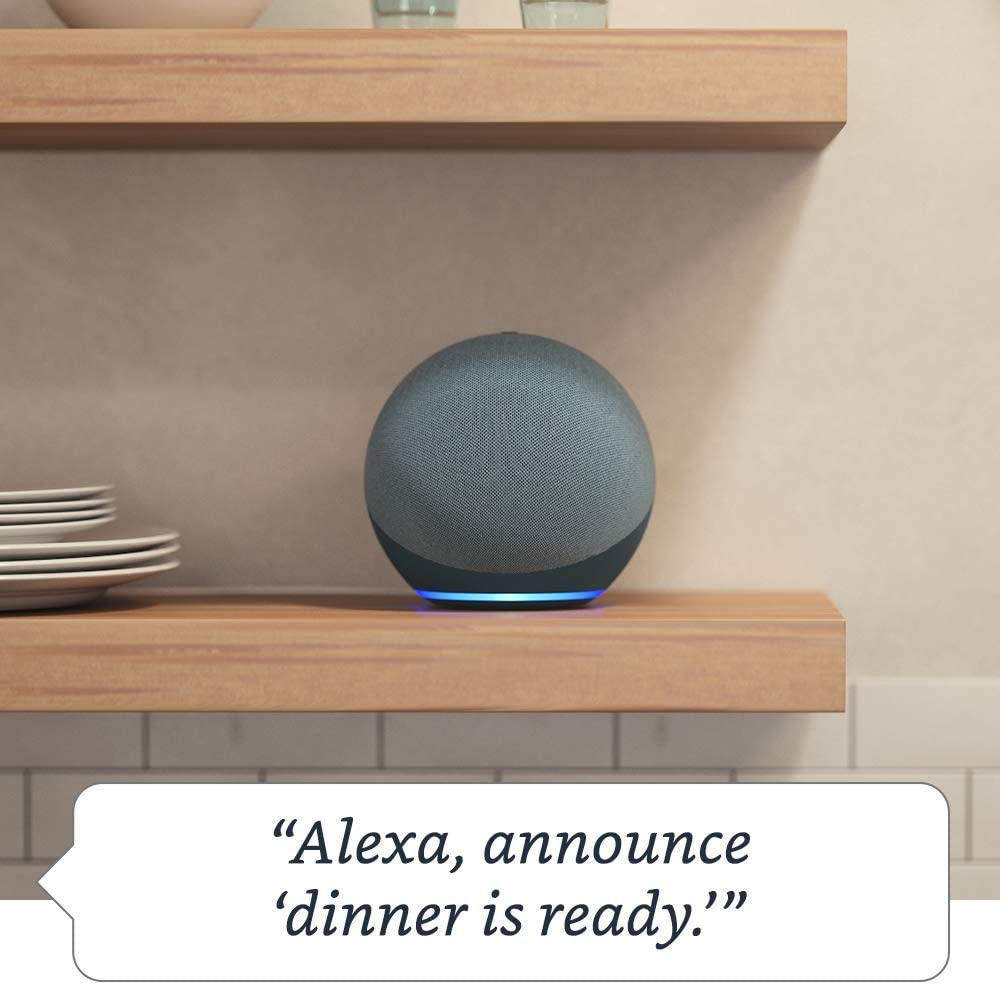
\includegraphics[width=0.4\textwidth]{./images/echodot4.jpg} % <- formatos PNG, JPG e PDF
    \fonte{Amazon (2022)}
	\label{fig:echodot4}
\end{figure}

\begin{quote}
    \textit{This device is a gem! When I’m busy in the kitchen, for example, and can’t get
    to a computer to find info or music to play, Alexa would be there to listen
    and do what I ask.} \\
    Customer review from \cite{GaoPanWangChen2018}
\end{quote}

Alongside the devices themselves, entirely new markets have emerged such as the
third-party software extensions called \textit{Alexa Skills} \cite{Alexa2022}.

These skills function much like mobile phone apps, extending and enhancing the
functionality of the device and can be sold to end users.

Developers can then easily leverage the highly advanced machine learning models
through Application Programming Interfaces (\sigla{API}{Application Programming
Interface}) and focus exclusively on their business logic, as shown on Figure
\ref{fig:alexaskill}.

This can be valuable as Machine Learning models are considered to be
expensive to develop and maintain, with some sources mentioning a minimum expenditure 
of US\$ 60.000 over a five year period considering both tasks \cite{Phdata2021}.

\begin{figure}[htb!]
	\centering
	\caption[Diagram showing the steps of an interaction with an Alexa Skill]{Diagram showing the steps of an interaction with an Alexa Skill}
	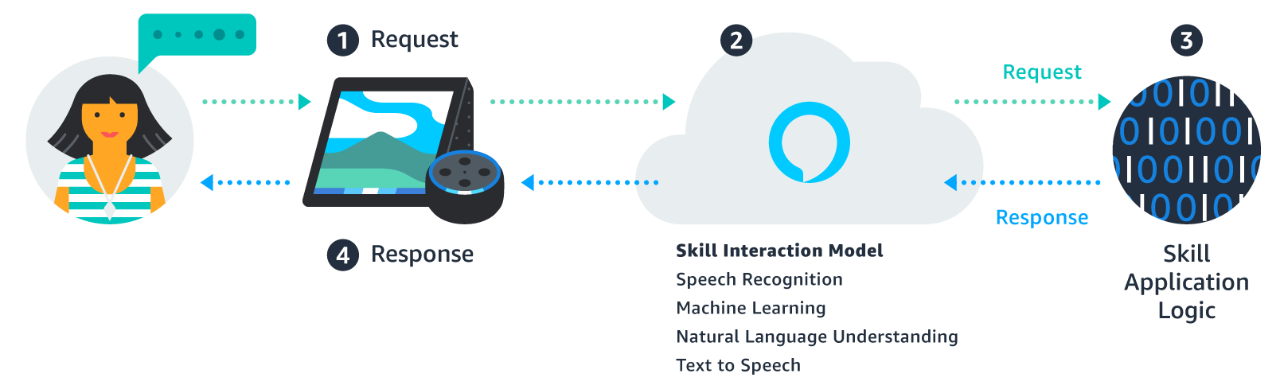
\includegraphics[width=0.9\textwidth]{./images/skills.png} % <- formatos PNG, JPG e PDF
    \fonte{\cite{Alexa2022}}
	\label{fig:alexaskill}
\end{figure}

More impressively, such technological advancements have been able to reach a
considerable amount of households in a short period of time in developed
countries like the United States, as shown on Figure \ref{fig:smartspeaker}.

\begin{figure}[H]
	\centering
	\caption[US Smart Speaker Penetration from 2017 to 2022]{US Smart Speaker Penetration from 2017 to 2022}
	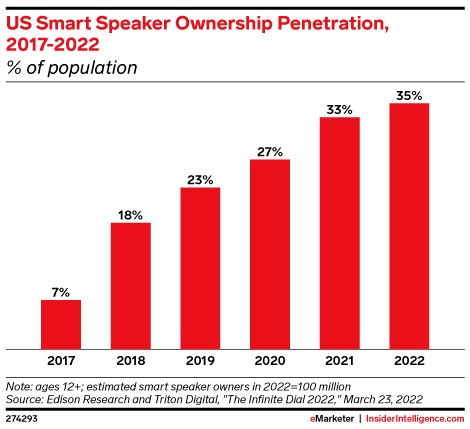
\includegraphics[width=0.6\textwidth]{./images/smartspeaker.png} % <- formatos PNG, JPG e PDF
    \fonte{\cite{InsiderIntelligence2022}}
	\label{fig:smartspeaker}
\end{figure}

On developing countries such as Brazil, these innovations tend to
have delayed arrivals due to historical economic barriers but the potential
customer base has attracted big tech companies like Amazon, which are able
to shorten the arrival delay with their economic power.

In Figure \ref{fig:alexabr}, we can see an example of a smart speaker advertisement 
from Amazon for the Brazilian customer base.

\begin{figure}[h!]
	\centering
	\caption[Localized promotional material for the Echo Show 10 targeting Brazilian customers]{Localized promotional material for the Echo Show 10 targeting Brazilian customers}
	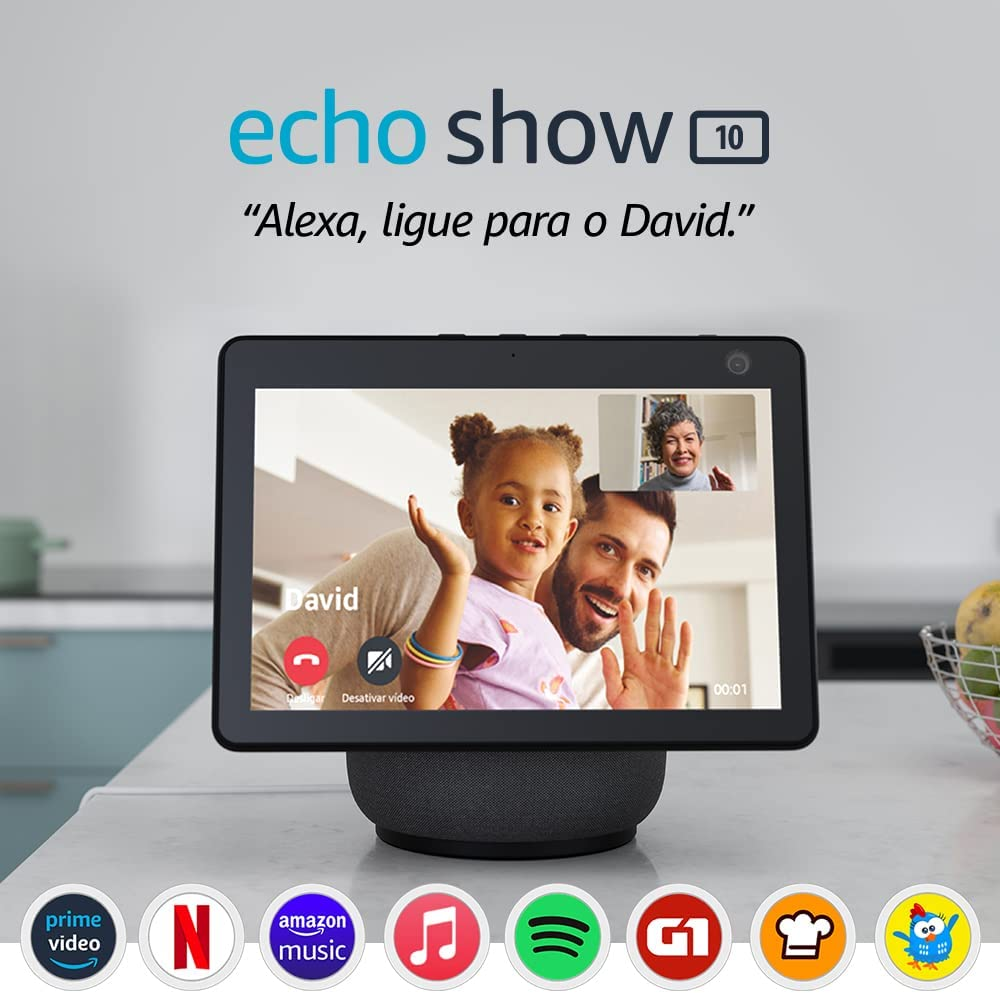
\includegraphics[width=0.4\textwidth]{./images/alexabr.jpg} % <- formatos PNG, JPG e PDF
    \fonte{Amazon (2022)}
    \label{fig:alexabr}
\end{figure}

According to the research company IDC Brasil, the Brazilian home automation
market -- in which smart speakers are included -- would have reached US\$ 291
million on 2021, an impressive figure that might explain the attractiveness of
our market \cite{IDCBrasil}.

But even with all of these innovations impacting customer behaviors day by day, one
important aspect of consumer life still has not had any significant changes in
the last couple of years: \textbf{shopping on
physical stores}.

According to \sigla{ABRAS}{Associação Brasileira de Supermercados} - the
Brazilian Supermarket Association - the Brazilian grocery retail sector has reached an
impressive total revenue of \textbf{R\$ 611 billion} in 2021 - roughly US\$ 117 billion on
October 2022 conversion rates - making up 7,03\% of the national \sigla{GDP}{Gross
Domestic Product}. About \textbf{28 million} customers visit one of the more than
\textbf{92.000} stores countrywide on a daily basis \cite{Abras2022}.

Despite all the technological advancement seen over the last few years and the
economic relevance of such sector, retail grocery shopping still exhibits the
same limitations found a decade ago. In a survey conducted in 2019, Capgemini
has found out five key pain problems related to physical stores in general
\cite{Capgemini2020}:

\begin{enumerate}
        \item Long queues for payment checkout
        \item Out of stock products
        \item Difficulties in locating products in the store
        \item Not being able to find a store associate to help
        \item Lack of product information when I select products
\end{enumerate}

The survey results can be seen in more detail in Figure \ref{fig:capgemini}.

\begin{figure}[H]
	\centering
    \caption[Top five customer pain points in retail stores]{Top five customer pain points in retail stores}
	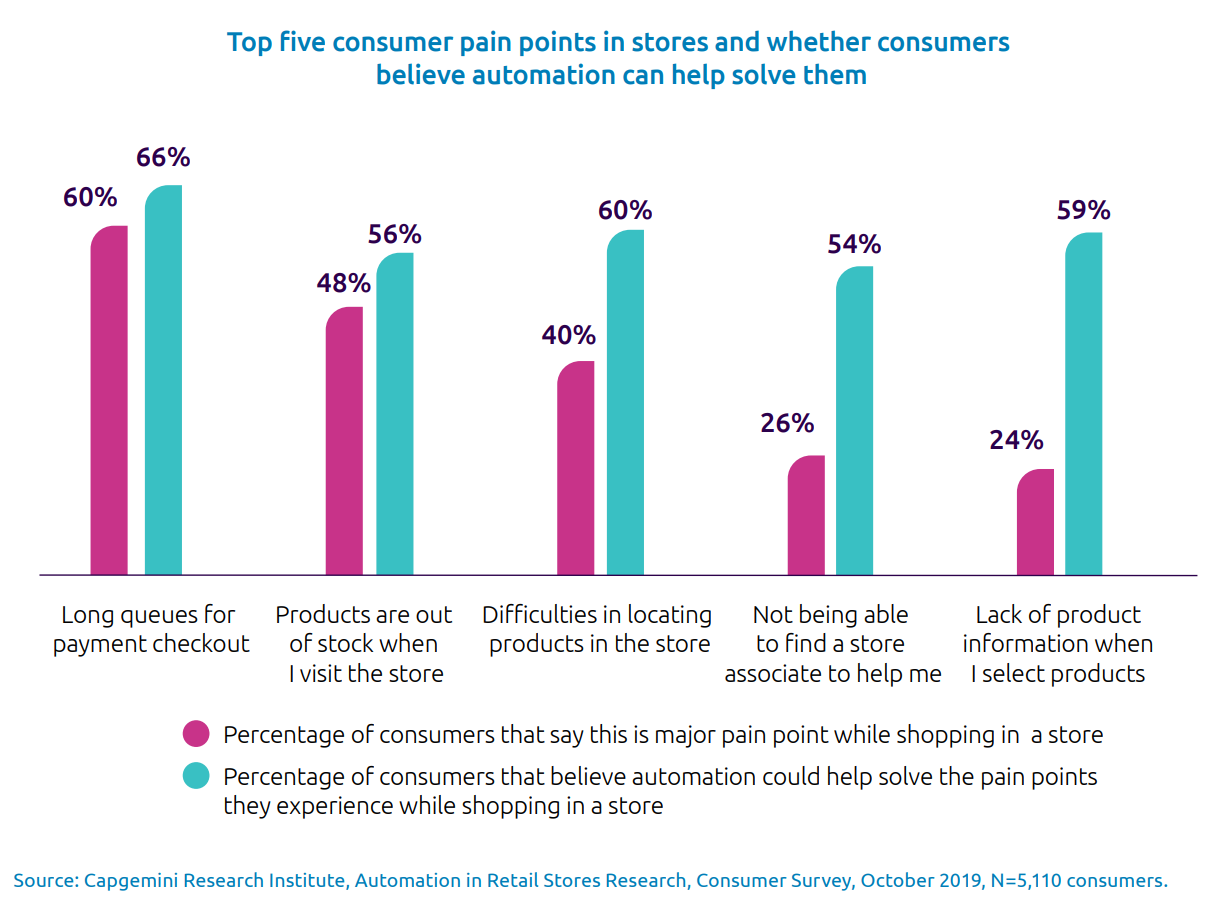
\includegraphics[width=0.8\textwidth]{./images/painpoints.png}
    \fonte{\cite{Capgemini2020}}
    \label{fig:capgemini}
\end{figure}

More interestingly, the survey points out that at least half of the survey
respondents believe that all of the five pain points can be solved through
\textbf{automation}. Even in light of the recent pandemic scenario, innovations
that increase automation such as e-commerce platforms had their adoption
increased in 2020 but 2021 showed a trend of consumers shifting
back to their pre-pandemic behavior, favoring physical retail stores
\cite{Kantar2022}.

It is in this scenario of customer pain and enormous market potential that this
thesis will explore a technological solution to improve customer experience and increase sales,
namely the \textbf{smart shopping cart}.

\section{Current scenario}

In this next section, we'll explore some of the existing solutions and the user experience
provided by them.

\subsection{Caper Cart}

Developed by the Caper\footnote{https://caper.ai} company, the Caper Cart was the worlds's first AI-powered smart cart \cite{Caper2020}

The first version was launched in 2017 and offered grocer's the
great advantage of not requiring any infrastructure overhaul for deployment.
In Figure \ref{fig:caperatretail}, we can see the cart deployed at American
retail store.

\begin{figure}[H]
	\centering
	\caption[Caper Cart at a retail store]{Caper Cart at a retail store}
	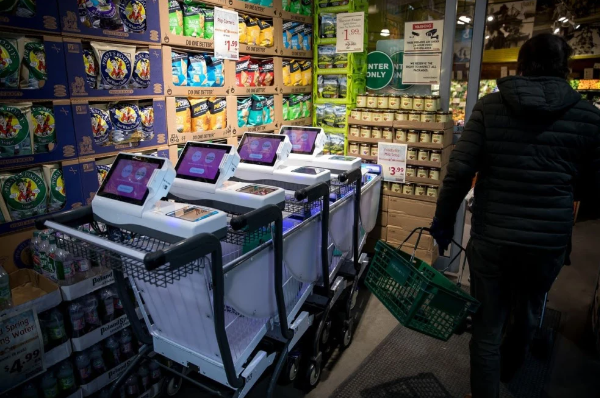
\includegraphics[width=0.7\textwidth]{./images/caper.png}
    \fonte{Caper (2020)}
	\label{fig:caperatretail}
\end{figure}

For end users, it offered visual product recognition and a payment terminal,
allowing them to avoid the dreaded queues by the end of their shopping session.
Additionally, customers were able to search products, get discounts and locate
items more easily with the help of the interactive user interface provided by the cart that 
can be seen on Figure \ref{fig:caperui}.

\begin{figure}[H]
	\centering
	\caption[Caper Cart user interface]{Caper Cart user interface}
	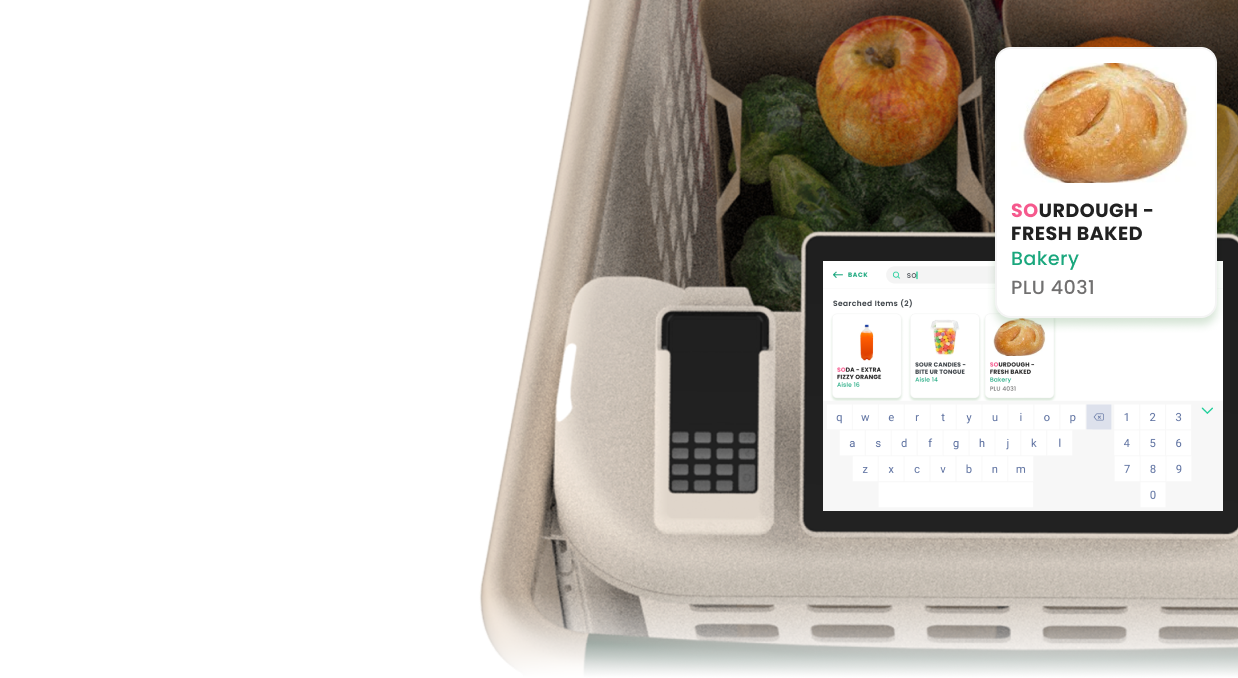
\includegraphics[width=0.7\textwidth]{./images/capercartui.png}
    \fonte{Caper (2020)}
	\label{fig:caperui}
\end{figure}

Although Caper does not publicize the cost of each cart, it is estimated that each unit costs between
\textbf{US\$ 5,000 and 10,000} \cite{TWP2021}.

Acquired by Instacart\footnote{https://instacart.com} in 2021 for US\$ 350
million, Caper is developing in 2022 the third version of its Smart Shopping
Cart, advertising an increase of \textbf{65\% in the basket volume} and a
\textbf{10 month} break even period, as shown on Figure \ref{fig:caperad}.

\begin{figure}[H]
	\centering
	\caption[Caper Cart 3 promotional material]{Caper Cart 3 promotional material}
	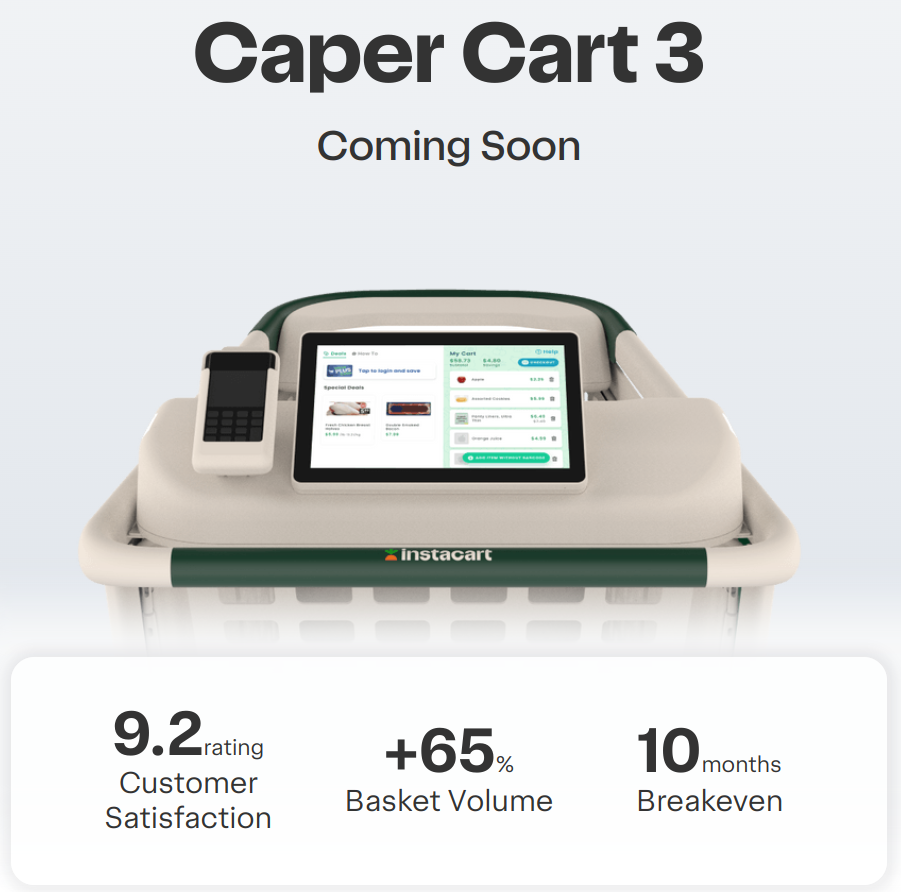
\includegraphics[width=0.7\textwidth]{./images/capercart3.png}
    \fonte{Caper (2022)}
	\label{fig:caperad}
\end{figure}


\subsection{Amazon Dash Cart}

Available at the Amazon Fresh\footnote{https://www.amazon.com/fmc/m/30003175?almBrandId=QW1hem9uIEZyZXNo} retail chain, the
Amazon Dash Cart is the company's first smart cart available to end users and is shown in
Figure \ref{fig:dashcart}.

According to Amazon, it uses computer vision and sensors to allow customers to
simply add items to their cart like they usually would. The cart accounts all
the items present in the cart, displaying a list which includes their prices
and subtotal. By the end of their item selection, customers can check-out
automatically without having to go through queues, solving the biggest customer
pain point pointed out by \cite{Capgemini2020}.

\begin{quote}
\textit{Looking to make grocery trips quicker? With the Amazon Dash Cart you can skip the checkout line and roll out to your car when you are done.}

\textit{The Dash cart uses a combination of computer vision algorithms and sensor fusion to help identify items placed in the cart - simply grab an item, scan it on one of the Dash Cart cameras, and place it in the cart like you normally would.}
\\
Amazon (2022)
\end{quote}

\begin{figure}[H]
	\centering
    \caption[Amazon Dash Cart]{Amazon Dash Cart}
	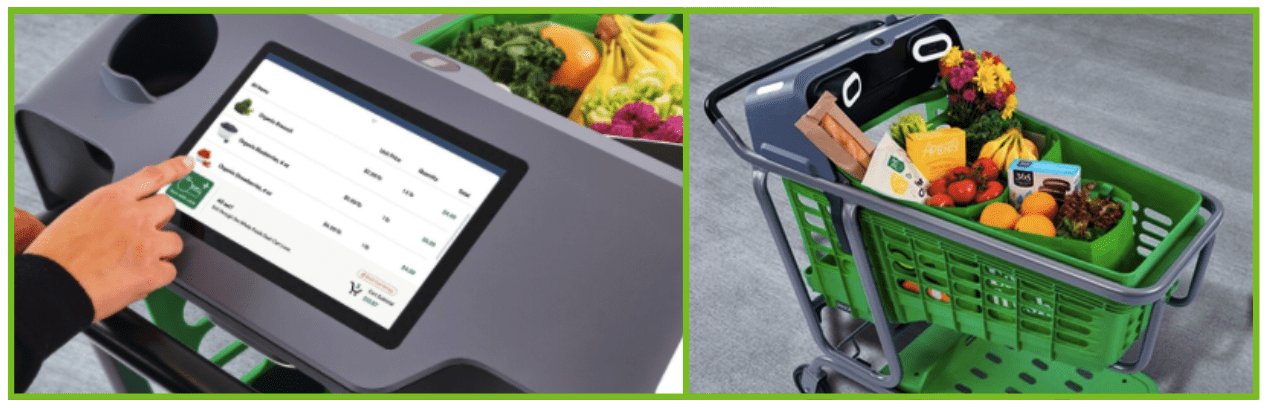
\includegraphics[width=0.8\textwidth]{./images/dashcart.png}
    \fonte{Amazon (2022)}
    \label{fig:dashcart}
\end{figure}

In addition to the item accounting capabilities, the user interface provided by
the Cart also allows customers to search for the location of items  in the
store and see more information about them, improving the customer experience.

One of its particularities is that it requires the download and usage of an mobile phone
app for using the cart, something not required by Caper's Cart.

As of October 2022, the Amazon Dash Cart is exclusively available at the Amazon
Fresh chain and therefore no commercial information regarding cost per unit is
available.

\subsection{Nextop}

Founded in 1997, Nextop\footnote{https://nextop.com.br} is a Brazilian company
that develops products with a focus on the grocery stores market, with an emphasis on
loss prevention.

Their smart cart offering, shown in Figure \ref{fig:nextop}, is the first
deployed in Brazil and Latin America according to the company and was
initially rolled out to the Enxuto supermarket chain in 2022
\cite{Paraiba2022}.

\begin{figure}[H]
	\centering
	\caption[Smart Cart Nextop® deployed to a Brazilian supermarket]{Smart Cart Nextop® deployed to a Brazilian supermarket}
	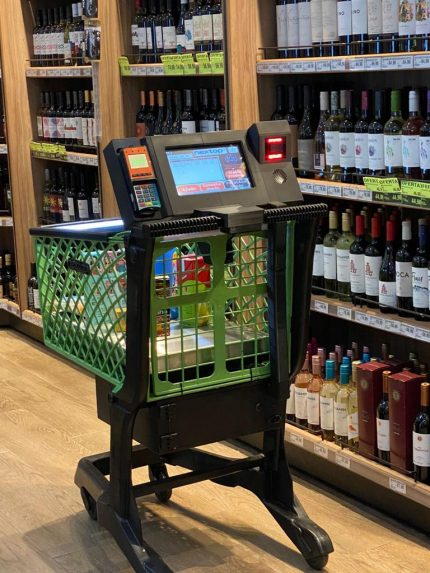
\includegraphics[width=0.4\textwidth]{./images/nextop.jpeg}
    \fonte{Nextop (2022)}
	\label{fig:nextop}
\end{figure}

In contrast to the carts developed by Amazon and Caper, Nextop's cart requires
an additional step of scanning the product using the integrated barcode reader,
shown in Figure \ref{fig:nextopui}, before adding it to the cart. With that, the
Nextop advertises for a \textit{triple validation} system, using the cameras,
sensors and the barcode scanner to prevent losses \cite{Nextop2022}.

\begin{figure}[H]
	\centering
    \caption[Smart Cart Nextop® user interface with a payment terminal]{Smart Cart Nextop® user interface with a payment terminal}
	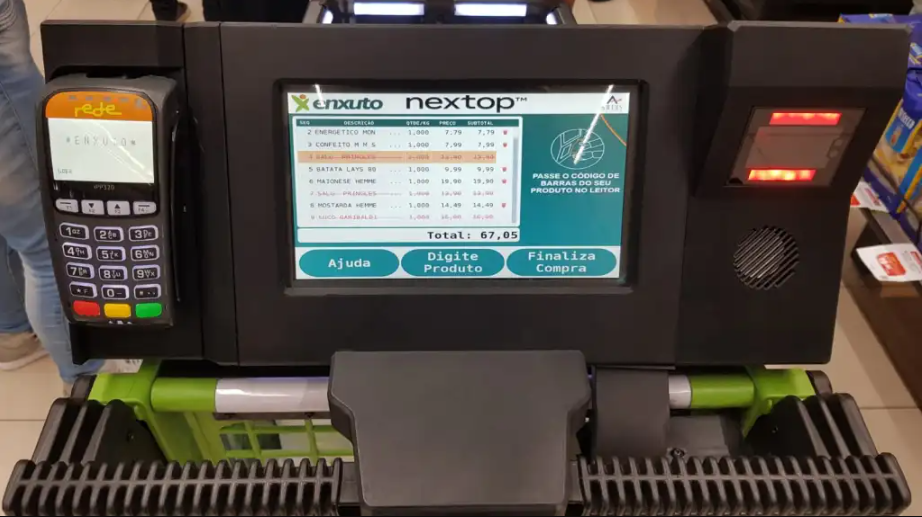
\includegraphics[width=0.9\textwidth]{./images/nextop2.png}
    \fonte{\cite{Paraiba2022}}
	\label{fig:nextopui}
\end{figure}

Although loss prevention is an important selling point for the Brazilian market,
the usage of the barcode scanner creates, in our opinion, a worse customer
experience, becoming a \textit{mobile checkout station}. Also, the product does not
include additional features such as product location search and item details. 

Figure \ref{fig:nextopad} shows an advertisement, in Portuguese, that lists the following
benefits:

\begin{itemize}
    \item Innovative supermarkets sell 20\% more
    \item Loss prevention
    \item Triple validation
    \item Freedom and agility
    \item New self checkout using artificial intelligence
    \item No queues
\end{itemize}

\begin{figure}[H]
	\centering
    \caption[Smart Cart Nextop® promotional material targetting supermarket owners]{Smart Cart Nextop® promotional material targeting supermarket owners. It advertises for improved sales, loss prevention and reduced queues.}
	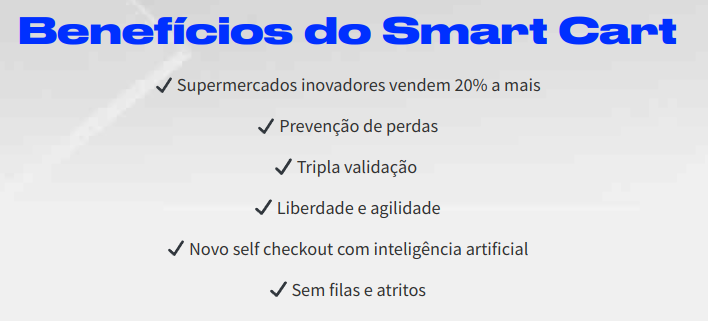
\includegraphics[width=0.9\textwidth]{./images/nextoppromo.png}
    \fonte{\cite{Nextop2022}}
	\label{fig:nextopad}
\end{figure}

Offering a solution to the main end user pain point of having to go through
long queues, the product also advertises increased sales as a result of the
innovative approach and also allows a deeper understanding of the customer
journey by collecting analytical data \cite{Paraiba2022}.

\begin{quote}
\textit{We are offering our customers an innovative and unique shopping experience within Enxuto}

\textit{With the smart cart, we broke through this barrier and managed to monitor the
entire customer's purchase circuit in the physical store. We have moved
from the identified ticket era to the end-to-end identified journey}

    Bruno Bragancini Junior, \sigla{CEO}{Chief Executive Officer} of the Enxuto Group \cite{Paraiba2022}
\end{quote}

According to Nextop's CEO, Juliano Camargo, the company has already invested \textbf{R\$ 8,5 millions} - about US\$ 1,63 million on October 2022 - and \textbf{4 and half years}
of research and development.

Each Smart Cart is estimated to cost around \textbf{R\$ 120,000} or around US\$ 23,020 on October 2022 \cite{Paraiba2022}.

\section{Objectives}

After presenting the problem domain and the current market scenario, in this section we discuss the 
objectives of this work.

\subsection{Main objective}
Develop a prototype of a smart shopping cart that utilizes computer
vision and sensor data for product recognition.

\subsection{Specific objectives}
\begin{itemize}
    \item Build a mechanical assembly for the prototype
    \item Develop an interactive user interface for the prototype
    \item Collect a product dataset for training a deep learning model
    \item Train a Deep Learning model capable of detecting target products
	\item Learn the practical challenges of developing a Deep Learning based product
    \item Understand the economic viability of such a project in the Brazilian context
\end{itemize}
%% Comente para remover este item

%% Capítulo
%%%% CAPÍTULO 2 - REVISÃO DA LITERATURA (OU REVISÃO BIBLIOGRÁFICA, ESTADO DA ARTE, ESTADO DO CONHECIMENTO)
%%
%% O autor deve registrar seu conhecimento sobre a literatura básica do assunto, discutindo e comentando a informação já publicada.
%% A revisão deve ser apresentada, preferencialmente, em ordem cronológica e por blocos de assunto, procurando mostrar a evolução do tema.
%% Título e rótulo de capítulo (rótulos não devem conter caracteres especiais, acentuados ou cedilha)
\chapter{Background}\label{cap:referencialTeorico}

In this section, we'll define in greater detail the theory behind some most
relevant techniques used in the development of the prototype.

This section can be skipped for readers with familiarity on the topics discussed.

\section{Neural Networks}

Neural Networks, or Artificial Neural Networks (\sigla{}{ANN}{Artificial Neural Network}),
are networks built out of interconnected decisional Neurons that aim to replicate 
the behavior of the human brain, enabling computational systems to cluster data
and to make predictions \cite{IBMNeuralNetworks}. 

A Neuron is similar to a Digital Logic Gate, which is capable of producing 
different outputs depending on the input signals that are sent to it.
A Neuron has weights, which are the coefficients that are used for calculating
the outputs; and biases, which are the boundaries that represent how prone is an output
to fit into a specific category of output. 

The main difference between a digital logic gate and a Neuron is that, because neurons are
parameterized with weights and biases, we can apply \textit{learning algorithms}
to tune (or train) Networks of Neurons using real world or synthetic data \cite{Nielsen2015}.

\subsection{Neurons}

One of the most popular types of Neurons is the Perceptron, introduced by 
\cite{Rosenblatt1958} and is shown in Figure \ref{fig:perceptron}. 
A perceptron takes one or more binary inputs and produces a single binary output.

\begin{figure}[H]
	\centering
	\caption[The Perceptron Neuron]{The Perceptron Neuron}
    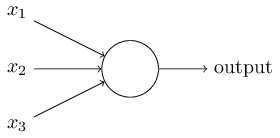
\includegraphics[width=0.5\textwidth]{./images/perceptron.png}
    \fonte{\cite{Nielsen2015}}
	\label{fig:perceptron}
\end{figure}

A Neuron does not necessarily have binary inputs and outputs. In fact,
contemporary systems commonly use a different type of Neuron known as the
Sigmoid Neuron, which take real numbers as inputs and also produces continuous
outputs within the boundaries of the sigmoid curve, shown in Figure
\ref{fig:sigmoid}, instead of discrete zeroes and ones.

This is particularly useful for learning, since in Perceptrons small differences in the 
weights or biases could yield to different outputs without a full transparency 
on how close the output would have been to a different one \cite{Nielsen2015}.

\begin{figure}[H]
	\centering
	\caption[Sigmoid Function]{Sigmoid Function}
    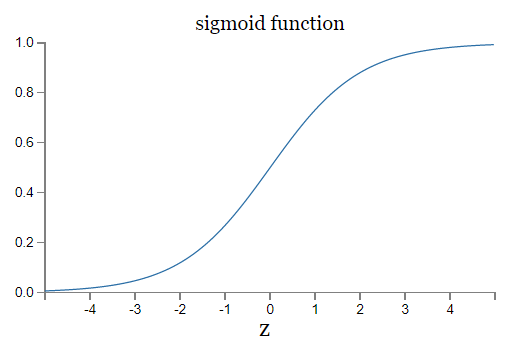
\includegraphics[width=0.5\textwidth]{./images/sigmoid-function.png}
    \fonte{\cite{Nielsen2015}}
	\label{fig:sigmoid}
\end{figure}

\subsection{Learning Algorithms}

There are three main types of learning algorithms: Supervised, Unsupervised and Reinforcement.
Supervised learning is employed when you know what are your expected outputs and use this
information to feed (train) your models such that they can start doing that on their own; 
Unsupervised learning is applied when you do not know what are the expected labels 
in your data or you do not have them available; and Reinforcement learning is used when
algorithms need to replicate specific behaviors depending on the feedback that is
provided to them \cite{CourseraML}. 

Supervised learning is typically employed for regression and classification tasks; 
Unsupervised Learning is typically used for clustering raw data into different buckets
without necessarily knowing how to do it or having the labelled data available;
and Reinforcement learning is often applied in control systems.
This work will primarily focus on Supervised Learning, since our proposed project uses
Object Detection and is trained based on labeled data samples.

As for the learning algorithms used for training Neural Networks, 
the standard algorithm is the Stochastic Gradient Descent (\sigla{SGD}{Stochastic Gradient Descent}).
Alike other gradient descent algorithms, the SGD aims to minimize the loss function of a given
Neural Network iteratively. In simple terms, it consists of an iterative optimization algorithm defined by an
objective function to minimize the error.

The key feature of the SGD is that it does that very efficiently by initializing the weights
and biases randomly and then fine tuning it during training by trying to find the higher descents 
(or the higher derivatives of the error function), reducing the number of necessary iterations, 
which is particularly important considering that the amount of data that is used to train AI
models has increased considerably over the last few years \cite{CornellSGD}.

Finally, in terms of the way how the SGD is computed in Neural Networks, a widely adopted approach 
for Supervised Learning is Backpropagation. Backpropagation computes the gradients of the final 
layers of a Neural Network first, and the gradients of the first layers at last, 
and it reuses partial computations of the gradient from a layer to the other to compute each layer's 
gradient, making it more efficient than calculating each layer's gradient separately \cite{BrilliantBackpropagation}. 

\section{Deep Learning}

Deep Learning defines a group of AI algorithms that use advanced learning techniques on the 
top of ANNs to train models that allow systems to forecast and clusterize data 
efficiently \cite{IBMDeepLearning}.
Deep Learning algorithms use Neural Networks that have three types of layers:
Input Layer, Hidden Layer and Output Layer, shown in Figure \ref{fig:threeLayeredAnn}.
        
\begin{figure}[H]
	\centering
	\caption[Three Layered Neural Network]{Three Layered Neural Network}
    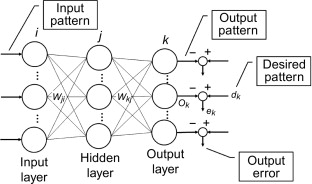
\includegraphics[width=0.6\textwidth]{./images/three-layered-ann.jpg}
    \fonte{\cite{ARAKI2015121}}
	\label{fig:threeLayeredAnn}
\end{figure}

The Input Layer takes the input data that will be fed into the model for training,
$x_i$, and produces the weighting coefficients $w_{ji}$. Input Layers
typically have the role of encoding the input data into a structure that can be processed by the 
subsequent hidden layers \cite{Paranjape2020}.

The $w_{ji}$ coefficients are then used to feed the Hidden Layer of the network,
which produces the weighting coefficients $w_{kj}$. The Hidden Layers of a Deep Learning 
Neural Network are used for the heavy processing of the encoded input data by applying a series of 
mathematical operations that ultimately makes it possible to break down the most important features
of the data and to produce comprehensive outputs to the decisional layers of the network
\cite{DeepAI_HiddenLayer}.

\subsection{Transfer Learning}

Another key technique applied by developers when training Deep Learning models is
\textit{Transfer Learning}. 
It consists of reusing pre-trained networks, which were tuned in other datasets -- usually big and
somehow related to the one that you are going to run your inferences on -- for training custom models.

Transfer Learning works by freezing the weights and biases present in specific layers of a
pre-trained Network -- usually being the hidden layers, which are the feature extractors -- 
when training customized models. This way,  only some layers of the Network -- usually the last layers, which 
are the deciders -- effectively have to be tuned.

The biggest advantages of Transfer Learning are that, because it allows for
training only specific layers of an architecture to get a custom model, the
training process is much faster than it would be if the whole network had to be
retrained; and additionally less training data is required for achieving a good
performing model, since you reuse the work done on the previous training
\cite{CS231N}.

\section{Object Detection}

Images can be processed as number matrices by computers, where each number represents a 
pixel's color level and each index points to a position in the image;
therefore, we can use collections of images as an input to train Deep Learning algorithms 
and perform classification and object detection tasks on them. 

Image Classification is a field of studies that is focused on labeling images
as a whole; Object Detection, on the other hand, focuses not only in
classifying them, but also in identifying the individual label's coordinates
within each image. For the purpose of our project and considering our proposed
product's specifications, we will focus on Object Detection, as it needs to be
able to recognize multiple objects within an image. 

To feed supervised Deep Learning algorithms to detect multiple objects in an
image, we need to provide our AI Models with images that have one or more
labels, the specification on what labels are there, and their coordinates. To
specify the coordinates of an object within an image, we use Bounding Boxes,
shown in Figure \ref{fig:boundingBoxes}. The Bounding Box also describes the
width and height of the object.

\begin{figure}[H]
	\centering
	\caption[Bounding Boxes]{Bounding Boxes}
    \includegraphics[width=0.4\textwidth]{./images/bounding-box.png}
    \fonte{\cite{AmazonRekognition}}
	\label{fig:boundingBoxes}
\end{figure}

For our models to perform feature extraction and ultimately be able to classify
each label in an image and tell their positions, an important mathematical
operation comes to play: the Convolution. Deep Learning algorithms that use
Convolutions in their backbones are typically called Convolutional Neural
Networks (\sigla{CNN}{Convolutional Neural Networks}). These algorithms
typically start by creating grid cells, which are delimiters for groups of
pixels, around the raw images for determining regions of interest and breaking
down concise representations of what are the elements within the image.
Convolutions are then applied from the original image against those grids to
filter and reduce the dimensionality of the original image and create feature
maps \cite{ObjectDetectionDeepLearning}. 

These feature maps then typically go through the final convolutional stages to
calculate Kernels that allows for creating activation functions around the grid
cells that contain each of the objects within the pictures \cite{JeremyJordan};
and those activation functions allow us to determine the Bounding Box
coordinates, the confidence score of the inference and the labels of the image
themselves. 

An example of that process is shown in Figure \ref{fig:convolutionActivation}.

\begin{figure}[H]
	\centering
	\caption[Activation Functions in Object Detection]{Activation Functions in Object Detection}
    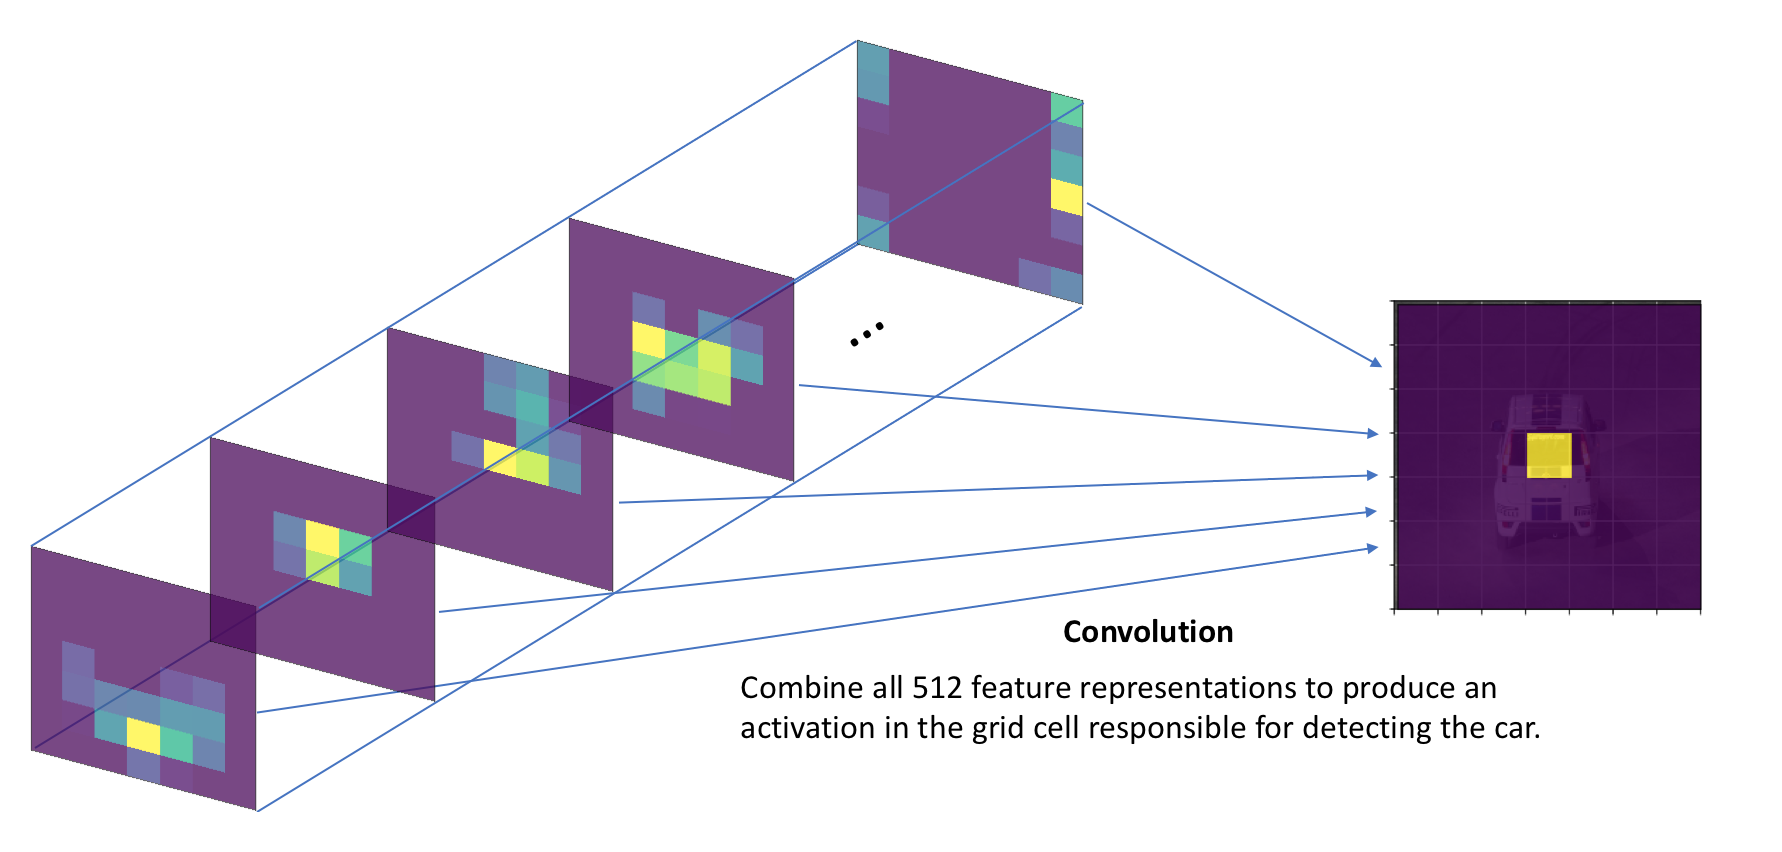
\includegraphics[width=1\textwidth]{./images/convolution-activation.png}
    \fonte{\cite{JeremyJordan}}
	\label{fig:convolutionActivation}
\end{figure}

Finally, a technique known as the Non-Maximum Suppression
(\sigla{NMS}{Non-Maximum Suppression}) is commonly used to filter the regions
of interest with the highest probability scores and ultimately get to a single
bounding box for each prediction. 
An example of the technique is shown in Figure \ref{fig:nmsObjectDetection}.

In this sense, two important metrics used for evaluating Object Detection models
are the Intersection over Union (\sigla{IoU}{Intersection over Union}), which measures 
the overlap between the predicted bounding box and the actual bounding box, 
as shown in Equation \ref{eq:IoU}; and the Average Precision, which measures the percentage 
of correct predictions made by the object detection model, as shown in Equation 
\ref{eq:AP}, where \textbf{True Positives} indicates the number of correct predictions and
\textbf{False Positives} measures the number of incorrect predictions made by the model.

\begin{equation}
\label{eq:IoU}
IoU = \frac{\text{Area of Overlap}}{\text{Area of Union}}=
\frac{
    \tikz{\fill[draw=blue, very thick, fill=blue!20] (0,0) rectangle (1,1) (0.5,-0.5) rectangle (1.5,0.5);
    \fill[draw=blue, very thick, fill=white, even odd rule] (0,0) rectangle (1,1) (0.5,-0.5) rectangle (1.5,0.5);}}
{\tikz{\fill[draw=blue, fill=blue!20, very thick] (0,0) rectangle (1,1) (0.5,-0.5) rectangle (1.5,0.5);}}
\end{equation}

\begin{equation}
	\label{eq:AP}
	AP = \frac{\text{True Positives}}{\text{True Positives + False Positives}}
\end{equation}


\begin{figure}[H]
	\centering
	\caption[NMS Applied to Object Detection]{NMS Applied to Object Detection}
    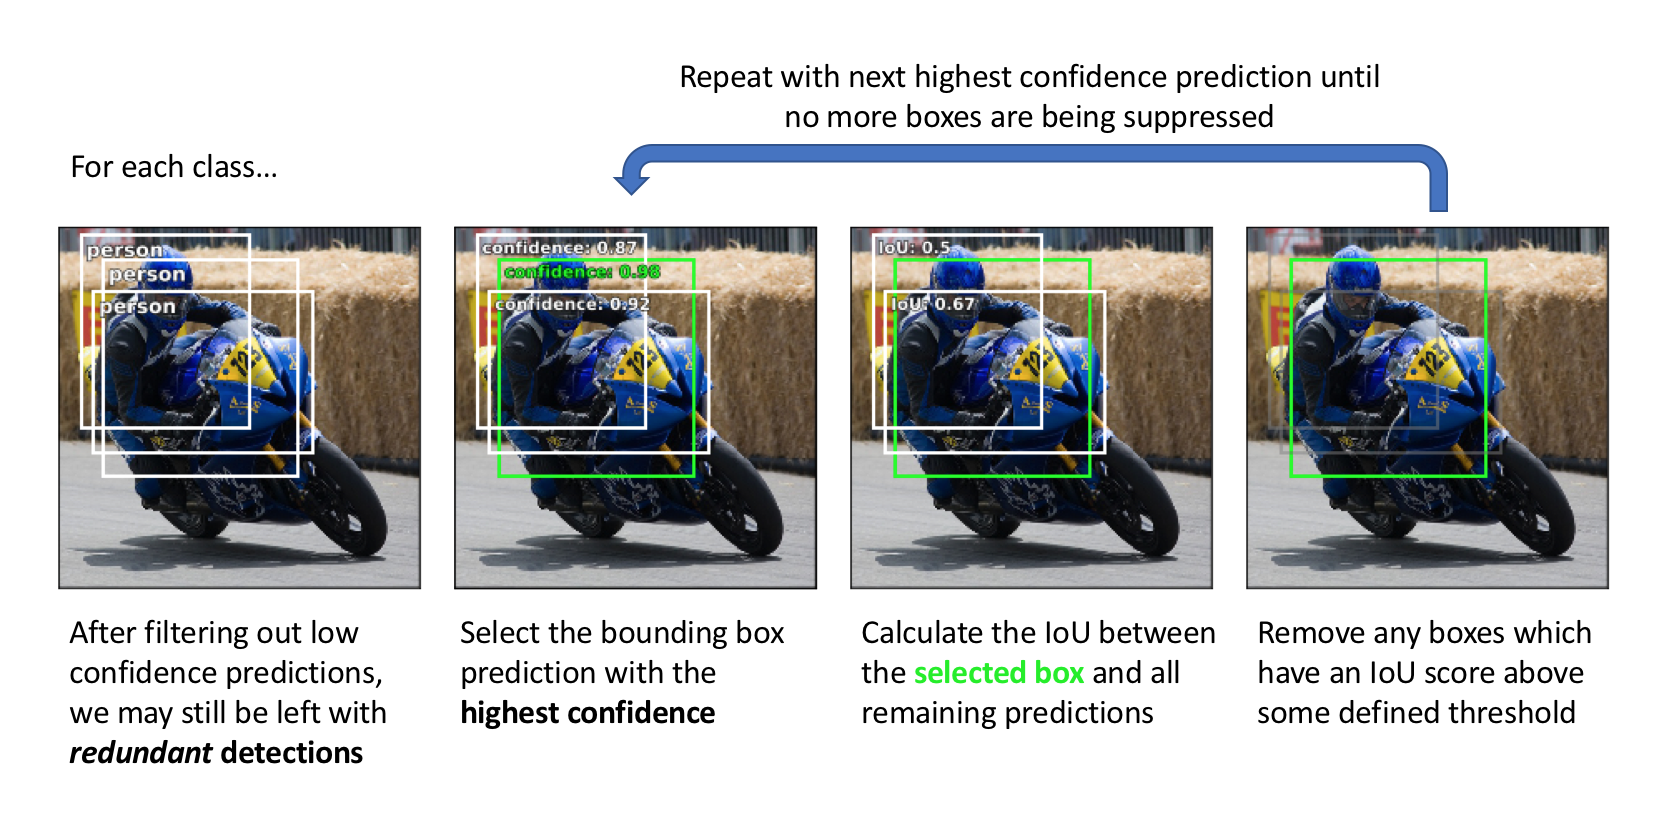
\includegraphics[width=1\textwidth]{./images/nms-object-detection.png }
    \fonte{\cite{JeremyJordan}}
	\label{fig:nmsObjectDetection}
\end{figure}

\section{Tensor Processing Unit}
\label{sec:TPU}

With the increased adoption of Deep Neural Networks (\sigla{DNN}{Deep Neural Networks}) 
in various workloads and their specialized and heavy compute nature, Google started the 
development of a domain specific architecture (\sigla{DSA}{Domain Specific Architecture}) 
which resulted in a first generation custom chip, named Tensor Processing Unit 
(\sigla{TPU}{Tensor Processing Unit}), deployed to their data centers since 2015 \cite{Google2015}.
The developed TPU had the target of improving the inference phase of DNNs and
achieved a performance improvement of \textbf{15-30 times} when compared to
contemporary hardware of paired or reduced power consumption. A block diagram of the TPU
architecture is shown in Figure \ref{fig:tpuarch}.

\begin{figure}[H]
	\centering
	\caption[TPU block diagram]{TPU block diagram. The main computation, matrix multiplication, is done by the yellow units.}
    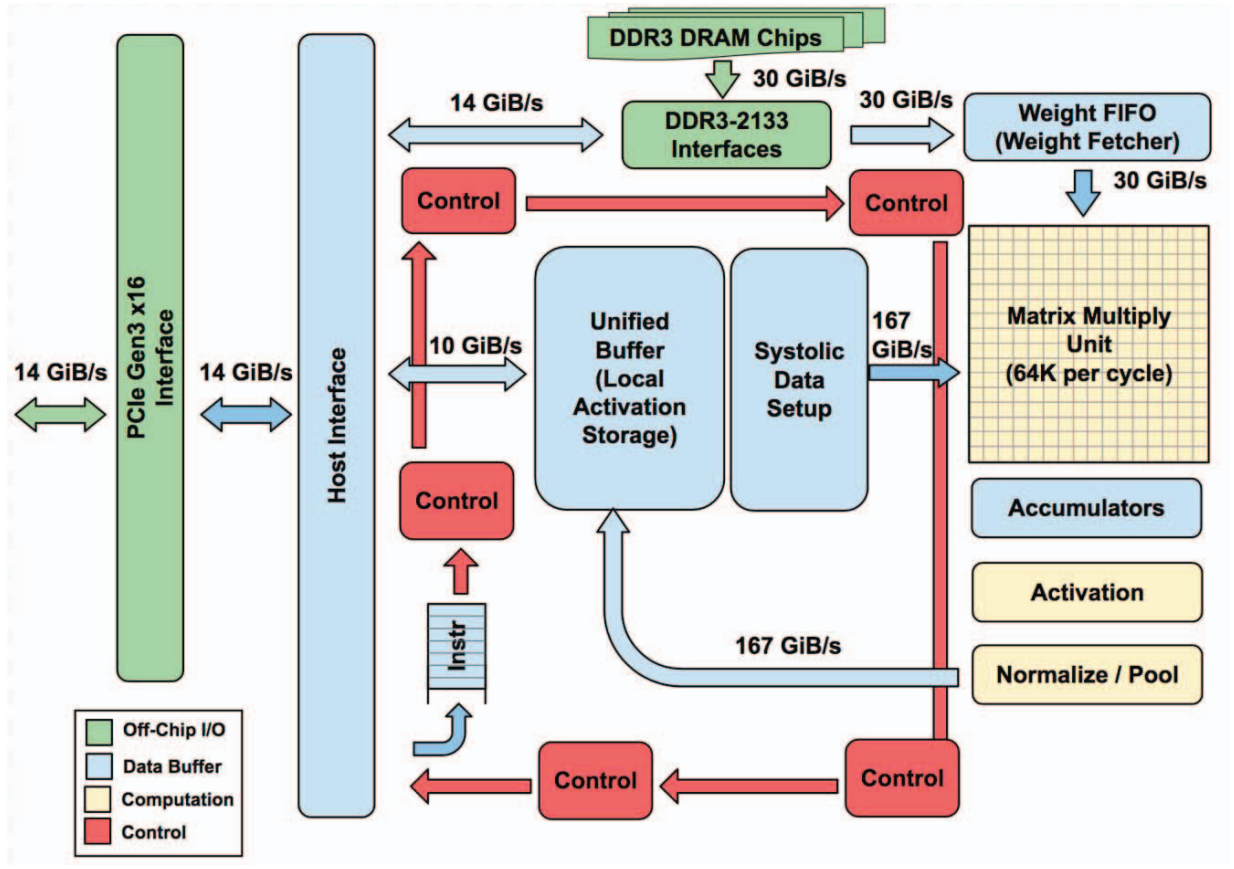
\includegraphics[width=0.6\textwidth]{./images/tpublock.png}
    \fonte{\cite{Google2015}}
	\label{fig:tpuarch}
\end{figure}

Since the first generation TPU described in a 2018 paper \cite{Google2015},
Google has released the TPU into commercials products made available to third
parties. Most notably, the Google Coral\footnote{https://coral.ai} initiative
offers ready-to-use development boards that embedded TPU chips, allowing
developers to leverage the improved DNN performance in their applications.

The Coral Dev Board Micro, an example of those ready-to-use boards is shown in
Figure \ref{fig:coraldev}.

\begin{figure}[H]
	\centering
	\caption[Coral Dev Board Micro]{Coral Dev Board Micro. It includes a microphone, camera and the Coral Edge TPU in a single board package.}
    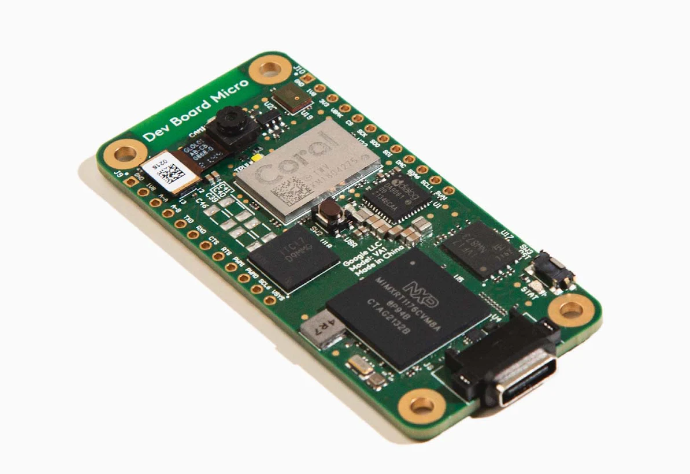
\includegraphics[width=0.5\textwidth]{./images/coralboard.png}
    \fonte{Coral.ai (2022)}
    \label{fig:coraldev}
\end{figure}

\section{Strain Gauge}

For measuring weight, one of the most common transducers used is the strain
gauge. A strain gauge is a device whose measured electrical resistance varies
with changes in its applied force, as a consequence of the mechanical
deformation \cite{Stefanescu}. A typical construction is shown in Figure 
\ref{fig:gauge1}.

\begin{figure}[H]
	\centering
	\caption[Typical Strain Gauge construction]{Typical Strain Gauge construction}
    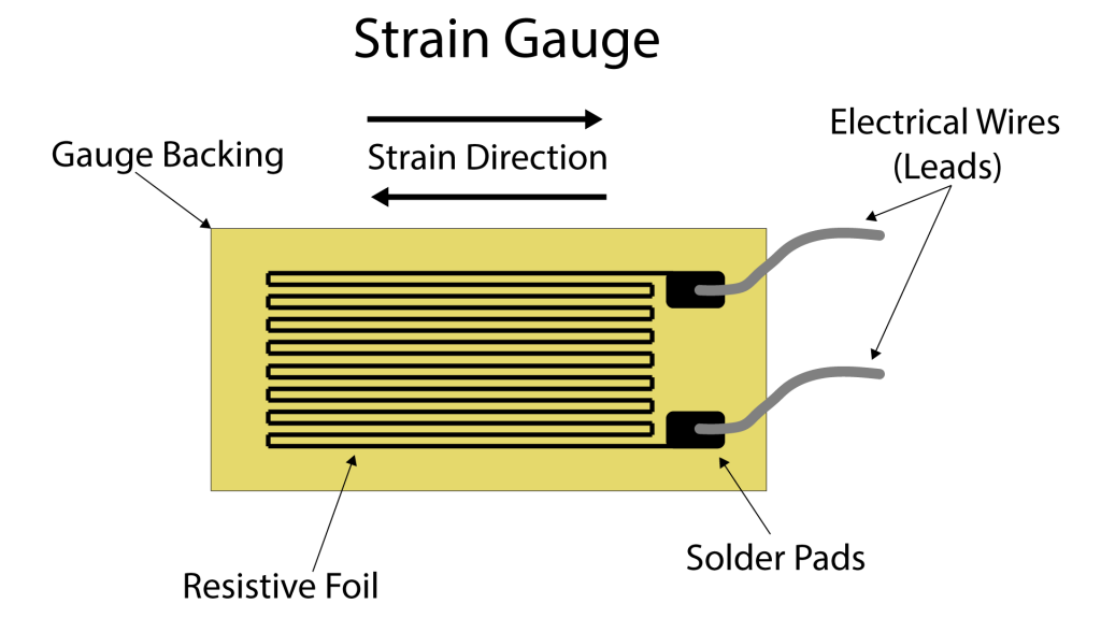
\includegraphics[width=0.5\textwidth]{./images/straingauge.png}
    \fonte{\cite{Michigan2020}}
	\label{fig:gauge1}
\end{figure}

In practice, however, the resistance variations observed after applying a
mechanical strain are minute and can be difficult to measure. To solve that issue,
and to also provide a signal which can be later used as the input of an
Analog-to-Digital Converter (\sigla{ADC}{Analog-to-Digital Converter}), the Wheatstone
Bridge circuit, shown in Figure \ref{fig:gauge2}, can be used \cite{Michigan2020}.

\begin{figure}[H]
	\centering
	\caption[Wheatstone Bridge circuit using four strain gauges]{Wheatstone Bridge circuit using four strain gauges}
    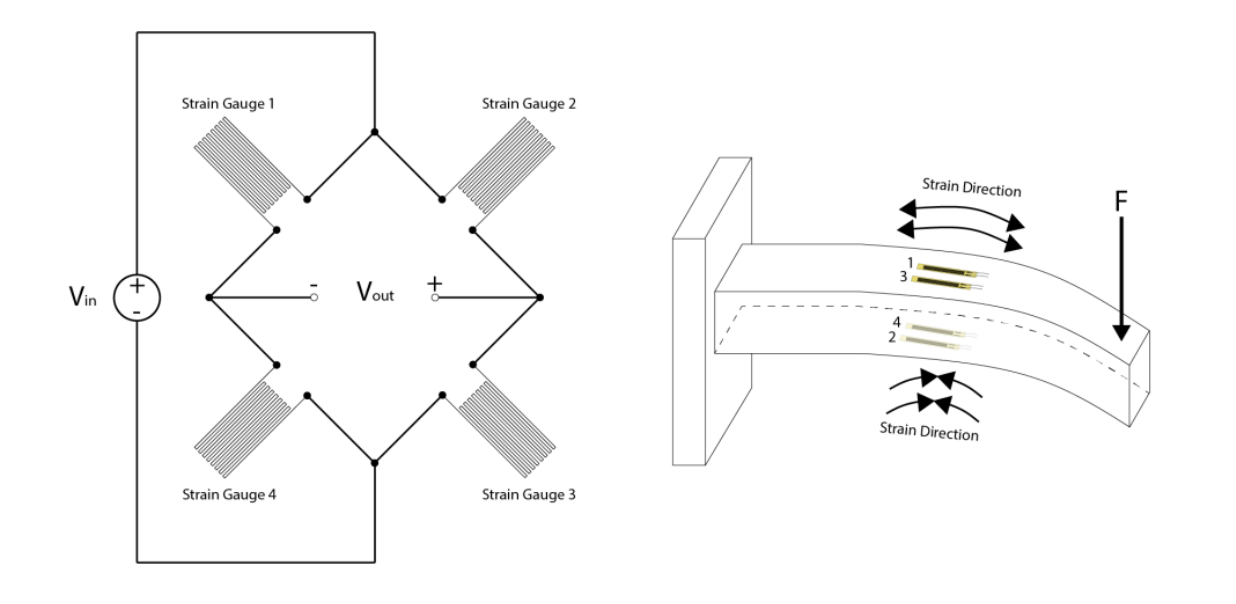
\includegraphics[width=0.9\textwidth]{./images/straingauge2.png}
    \fonte{\cite{Michigan2020}}
	\label{fig:gauge2}
\end{figure}

When no load is applied, the bridge is balanced and the output voltage
$V_{out}$ should be zero. If any strain is applied to the gauges, the bridge
will become unbalanced, and therefore will result in a non-zero output voltage.
Since the voltage variation tends to be small, in the order of millivolts, signal amplification is usually
required for pairing the bridge with commercially available ADCs \cite{HorowitzHill2015}.

It can be shown that the relation between $V_{out}$ and $V_{in}$, $S$, shown on Figure \ref{fig:gauge2}, can be
calculated as \cite{Stefanescu}:

\begin{equation}
    \label{eq:strain}
    S = \frac{V_{out}}{V_{in}} = k\frac{\Delta l}{l}
\end{equation}
where $k$ is known as the \textit{gauge factor}, related to the physical
construction and materials of the strain gauge, and $\frac{\Delta l}{l}$ is the
relative variation of length or strain.

With that, Equation \ref{eq:strain} indicates that the output voltage $V_{out}$
will be linearly proportional to the amount of strain applied, providing the
desired sensing capability.

\section{Load Cell}

Using strain gauges directly can be difficult since a proper
mechanical structure and arrangement is crucial for the sensors to function
properly. For that, commercially available \textit{Load Cells} offer ready to
use mechanical packages that embed the strain gauges for weight sensing
using electronic circuits.

In general, they consist of a spring element onto which the gauges are placed.
When load is applied to the cell, the strain gauges will be stressed and
therefore provide the desired sensing \cite{HBM2022}.

\begin{figure}[H]
	\centering
	\caption[HBM Z6 commercial load cell]{HBM Z6 commercial load cell}
    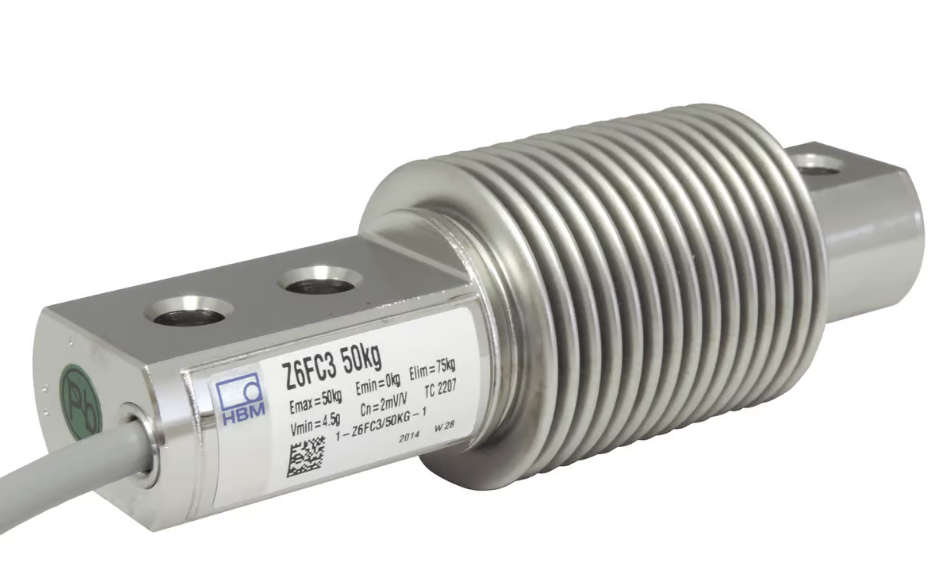
\includegraphics[width=0.3\textwidth]{./images/hbmz6.png}
    \fonte{HBM (2022)}
	\label{fig:gauge2}
\end{figure}
%% Comente para remover este item

%% Capítulo
\chapter{Development} \label{chap:desenv}

In this section, we describe the development of the \textit{zCart} smart cart
prototype. All the source code related to the prototype is available at a
GitHub repository\footnote{https://github.com/fsmiamoto/zcart}

\section{Design}
\label{sec:design}

As a first step in developing our prototype, a set of
high level goals was defined to guide the initial technical design:

\begin{enumerate}
    \item Handle user interactions and give visual feedback
    \item Store the current set of products present in the cart and their respective information
    \item Recognize the addition or removal of products, including quantities.
\end{enumerate}

With those goals in mind, the high level architecture of the prototype
was designed and is shown in Figure \ref{fig:architecture}.

For each goal, a dedicated software application will be used and those
applications will communicate using \siglaPt{TCP}{Transmission Control Protocol}
network sockets \cite{Kurose2013} with industry standard application protocols such as
\siglaPt{HTTP}{Hypertext Transfer Protocol}\footnote{First defined in
\siglaPt{RFC}{Request For Comments} 1945} and WebSocket\footnote{Defined in RFC 6455}.
Most of the HTTP communication will follow the widespread REST pattern \cite{Roy2000}.

\begin{figure}[H]
	\centering
	\caption[High level architecture of zCart]{High level architecture of zCart}
    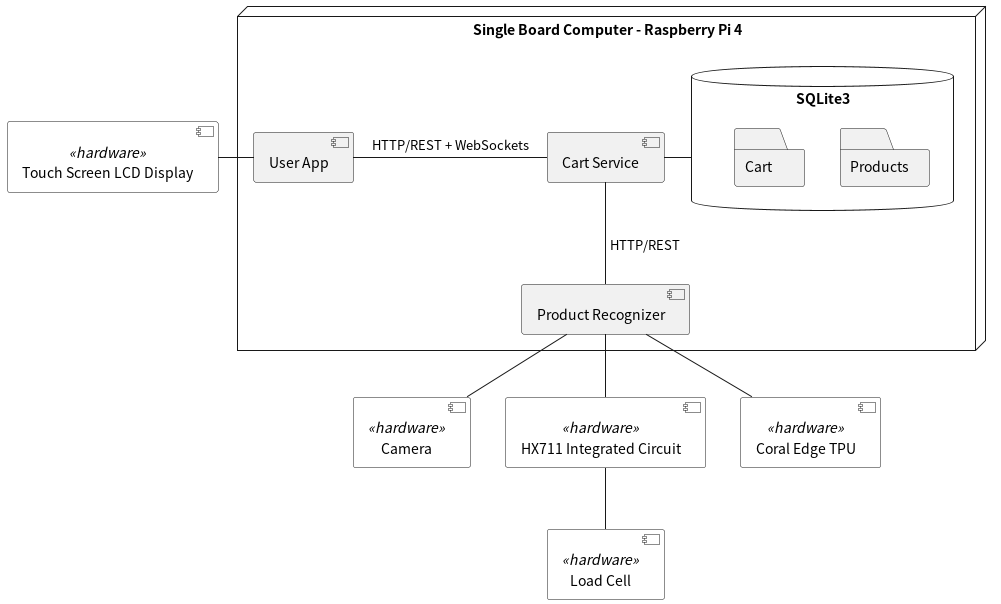
\includegraphics[width=1\textwidth]{./images/zCart.png}
	\fonte{}
	\label{fig:architecture}
\end{figure}

For handling the first goal, the \textit{User App} will request data
from other applications and will display the information to end users and allow
them to interact with the cart using a touch enabled LCD display. 

The \textit{Cart Service} will be in charge of the second goal,
handling requests from the \textit{User App}, which asks for data 
on the products that are detected and notifies the completion of a purchase order 
when the user completes the checkout. The \textit{Cart Service} uses a
\textbf{relational database} \cite{Silberschatz2010} as its primary database. Namely
\textbf{SQLite}, considered to be the world's most deployed database due to its
massive adoption on mobile
devices\footnote{https://www.sqlite.org/mostdeployed.html}. The simplicity of
SQLite, the entire database is contained within a single file, great
library support on common programming languages and the use of the familiar
relational modeling, including \siglaPt{SQL}{Structured Query Language}
\cite{Nield2016}, were key factors in choosing it.

In order to provide real time updates to the \textit{User App}, the Cart Service has a
WebSocket API endpoint that allows the User App to listen to updates such as a product addition
and then display a notification to the end user.

For the third goal, the \textit{Product Recognizer} application will be responsible
for processing a camera feed and weight sensor data to be able to tell if any products
were added of removed from the cart. Any detected changes will be communicated to the
Cart Service, which will be responsible for persisting those changes on the database. 

All three applications will execute under a Linux \cite{Tanenbaum2015} 
based environment on a Raspberry Pi\footnote{https://www.raspberrypi.com} 4 Single Board
Computer (\siglaPt{SBC}{Single Board Computer}) - a complete computer built on a single 
circuit board with a microprocessor, memory and input/output devices.

The advantages of using a Linux environment for the development are many, but
being able to leverage its concurrency capabilities, having built-in drivers
for readily available hardware and leveraging open source projects are some 
worth mentioning.

An End-to-End sequence diagram of an example action is shown in Figure \ref{fig:e2eseq}.

\begin{figure}[H]
	\centering
	\caption[End-to-end sequence diagram for a product addition]{End-to-end sequence diagram for a product addition}
    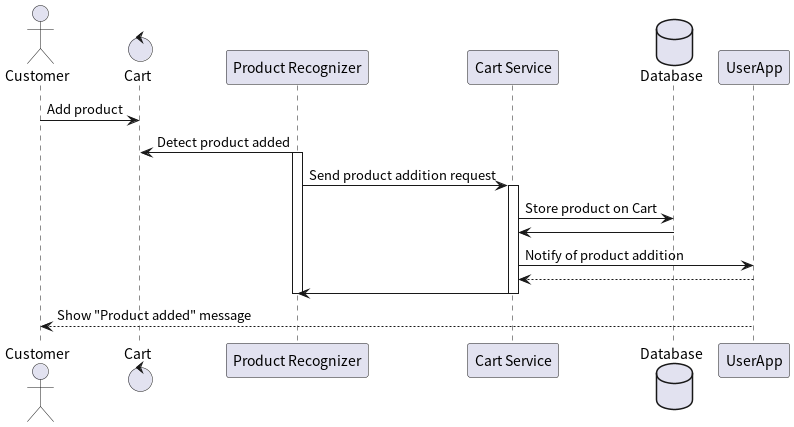
\includegraphics[width=1\textwidth]{./images/E2E.png}
	\fonte{}
	\label{fig:e2eseq}
\end{figure}

\subsection{Architectural Guidelines}
In creating the zCart architecture, the following guidelines were followed:

\begin{itemize}
    \item Create a separate software application for each goal domain
    \item Use well defined standards for communication between applications.
    \item All databases should be owned by a single application. 
    \item Any interaction that requires an update to a given database that is
        not owned by an application should be done through an API and not
        directly on the database.
    \item Decouple the user interface from how the data displayed is stored and transmitted
\end{itemize}

These guideline are based on known best practices from the software 
development industry including API-first design and segregation of
responsibilities \cite{Sam2021,Kong2022}, which are key for future architectural
evolution.

In the next sections, each application will be discussed in further detail.

\section{User App}

For developing the User App, we have used web technologies such 
as HTML, CSS \cite{Duckett2011} and JavaScript \cite{Flanagan2020} using the 
React\footnote{htps://reactjs.org} framework. 

Using web-based technologies allows the User App to be displayed on any 
device capable of running a web browser; and having mature tooling for 
development, testing and debugging are important factors that influenced 
our decision.

As an alternative, developing Linux native graphical applications through
toolkits such as GTK\footnote{https://gtk.org} and Qt\footnote{https://qt.io}
might have yielded better performance but our unfamiliarity with those would be
a challenge.

\begin{figure}[H]
	\centering
	\caption[User App Interface display a single product]{User App Interface displaying a single product}
    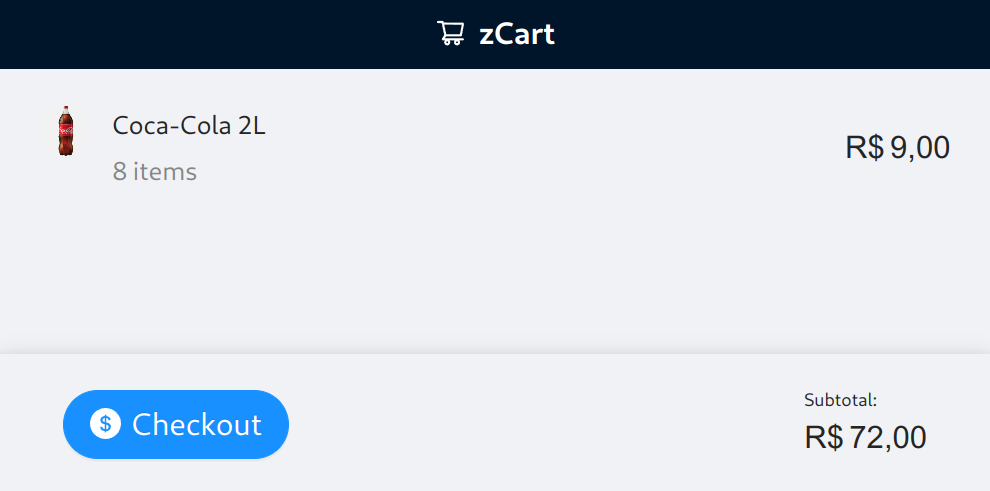
\includegraphics[width=0.8\textwidth]{./images/ui.png}
	\fonte{}
	\label{fig:userapp}
\end{figure}

As shown in Figure \ref{fig:userapp}, the main objective of the User App is to
provide a visual feedback mechanism for end users of the zCart. It displays the
current products added to the cart, their amounts and also the price for each
item. The subtotal price for all products added to the cart is calculated and
also displayed on the interface. Notifications are also displayed when the user
adds or removes a product from the cart. 

Finally, the User App provides a \textit{Checkout} button to simulate the payment process
and act as a Proof-of-Concept (\siglaPt{PoC}{Proof-of-Concept}), since a functional
implementation of a payment mechanism is out of scope for our prototype.

More screenshots showing the user experience are available in Appendix \ref{ap:userapp}.

In terms of the data flow, the User App requests all data from the Cart
Service, which exposes API endpoints for getting the list of products of a
given cart, establishing a WebSocket connection for notifications and
performing the PoC checkout. Figure \ref{fig:userappdataflow} displays the
endpoints of the Cart Service used by User App.

\begin{figure}[H]
	\centering
	\caption[User App and Cart Service interactions]{User App and Cart Service interactions}
    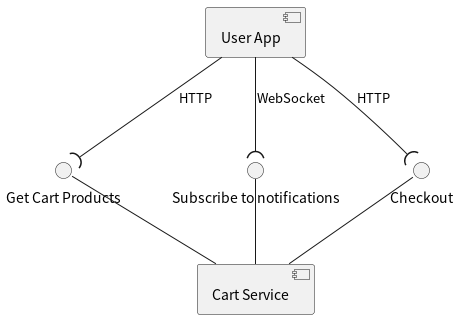
\includegraphics[width=0.6\textwidth]{./images/diagrams/UserApp.png}
	\fonte{}
	\label{fig:userappdataflow}
\end{figure}

\section{Cart Service}

As described in Section \ref{sec:design}, the Cart Service will act as a
centralized storage of the overall \textbf{state} of the cart.

For that, it will responsible for managing the SQLite database and exposing API
endpoints for the required state changes e.g. adding a product, as shown in 
Figure \ref{fig:cartservicearch}.

\begin{figure}[H]
	\centering
    \caption[Cart Service architecture]{Cart Service architecture. The database
    is contained withing the Cart Service boundary and it is not exposed in the
    public APIs}
	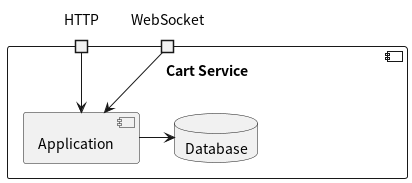
\includegraphics[width=0.6\textwidth]{./images/diagrams/CartService.png}
	\fonte{}
	\label{fig:cartservicearch}
\end{figure}

For the HTTP endpoints, the application uses the REST \cite{Roy2000} pattern
with JavaScript Object Notation (\siglaPt{JSON}{JavaScript Object
Notation})\footnote{https://json.org} as the data-interchange format, both
being widely employed in the software industry. Table \ref{tab:cartendpoints} displays all the API
endpoints created.

\begin{table}[H]
	\centering
    \caption[Cart Service API endpoints]{Cart Service API Endpoints.}
	\begin{tabular}{c | c|c}
		\hline 
        HTTP Method & URI & Description \\
		\hline
        \texttt{GET} & \texttt{/cart/:cartId} & Get the cart data with the product listing \\
        \texttt{POST} & \texttt{/cart/:cartId/products} & Add or remove a product from the cart \\
        \texttt{POST} & \texttt{/cart/:cartId/checkout} & Perform checkout, emptying the cart \\
		\hline 
	\end{tabular}
	\fonte{}
    \label{tab:cartendpoints}
\end{table}

An example response of the \texttt{GET /cart/:cartId} endpoint is shown in
Listing \ref{lst:response}.

\begin{sourcecode}
\caption{Example response for the \texttt{GET /cart/:cartId} endpoint using JSON}
\begin{lstlisting}[label={lst:response}]
{
  "id": "1",
  "products": [
    {
      "cart_id": "1",
      "product_id": "1",
      "quantity": 11,
      "product": {
        "id": "1",
        "name": "Coca Cola",
        "description": null,
        "price": 5.99,
        "image_url": "https://zcart-test-images.s3.amazonaws.com/coca2l.png"
      }
    },
  ]
}
\end{lstlisting}
\fonte{}
\end{sourcecode}

For implementing the Cart Service, the Go\footnote{https://go.dev} programming
language was used alongside the Fiber\footnote{https://gofiber.io/} framework,
which provides great support for the creation of a HTTP Server and also
handling the WebSocket connections.

One of the advantages of the Go language is the use of statically compiled
native binaries, which allows running the application without the need to
install any additional operating system libraries on the Linux environment. 

\section{Product Recognizer}

At the core of the zCart prototype is the Product Recognizer application,
responsible for the product detection based on computer vision and weight
sensing.

For achieving its goal, the Product Recognizer has three main components, as shown in Figure
\ref{fig:productrecognizerarch}.

\begin{figure}[H]
	\centering
	\caption[Product Recognizer Components]{Product Recognizer Components. Detected events will be communicated to the Cart Service for persistence}
    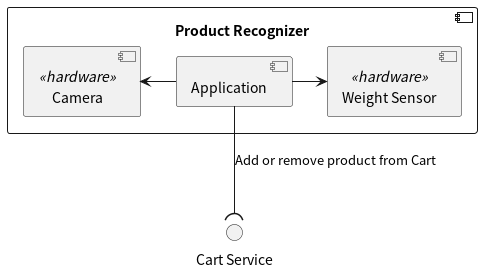
\includegraphics[width=0.6\textwidth]{./images/diagrams/ProductRecognizer.png}
	\fonte{}
	\label{fig:productrecognizerarch}
\end{figure}

Each of these components will be described in more detail in the next subsections.

\subsection{Weight Sensor}

For the Weight Sensor, we've used two main hardware components, shown on Figure \ref{fig:weighttesting}:
\begin{itemize}
    \item  A 10 Kilogram Load Cell
    \item HX711 Integrated Circuit
\end{itemize}

The HX711 is a 24-bit analog-to-digital converter (\siglaPt{ADC}{Analog-to-Digital Converter})
capable of outputting data in a serial interface \cite{Avia2022}.

It has two channels for analog input with channel A having programmable gains of 128 or 64 and
can function using both 3.3V and 5V standard digital voltage levels. The pinout is shown
in Figure \ref{fig:hx711pinout}.

One of its advantages is is that there's no need to program internal registers,
all controls to the chip are through its pins. Additionally, it consumes only
1,5 mA under normal operation and has an on-chip power supply for the connected
load cell, making it a great choice for our prototype.

\begin{figure}[H]
	\centering
	\caption[HX711 Pinout for the SOP-16L package]{HX711 Pinout for the SOP-16L package}
    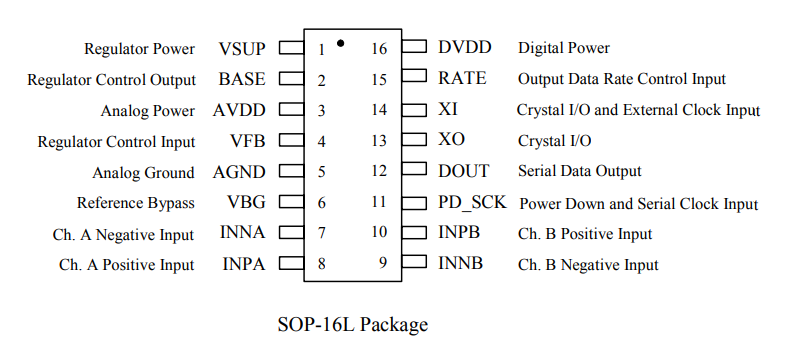
\includegraphics[width=0.9\textwidth]{./images/hx711-pinout.png}
    \fonte{\cite{Avia2022}}
	\label{fig:hx711pinout}
\end{figure}

\begin{figure}[H]
	\centering
	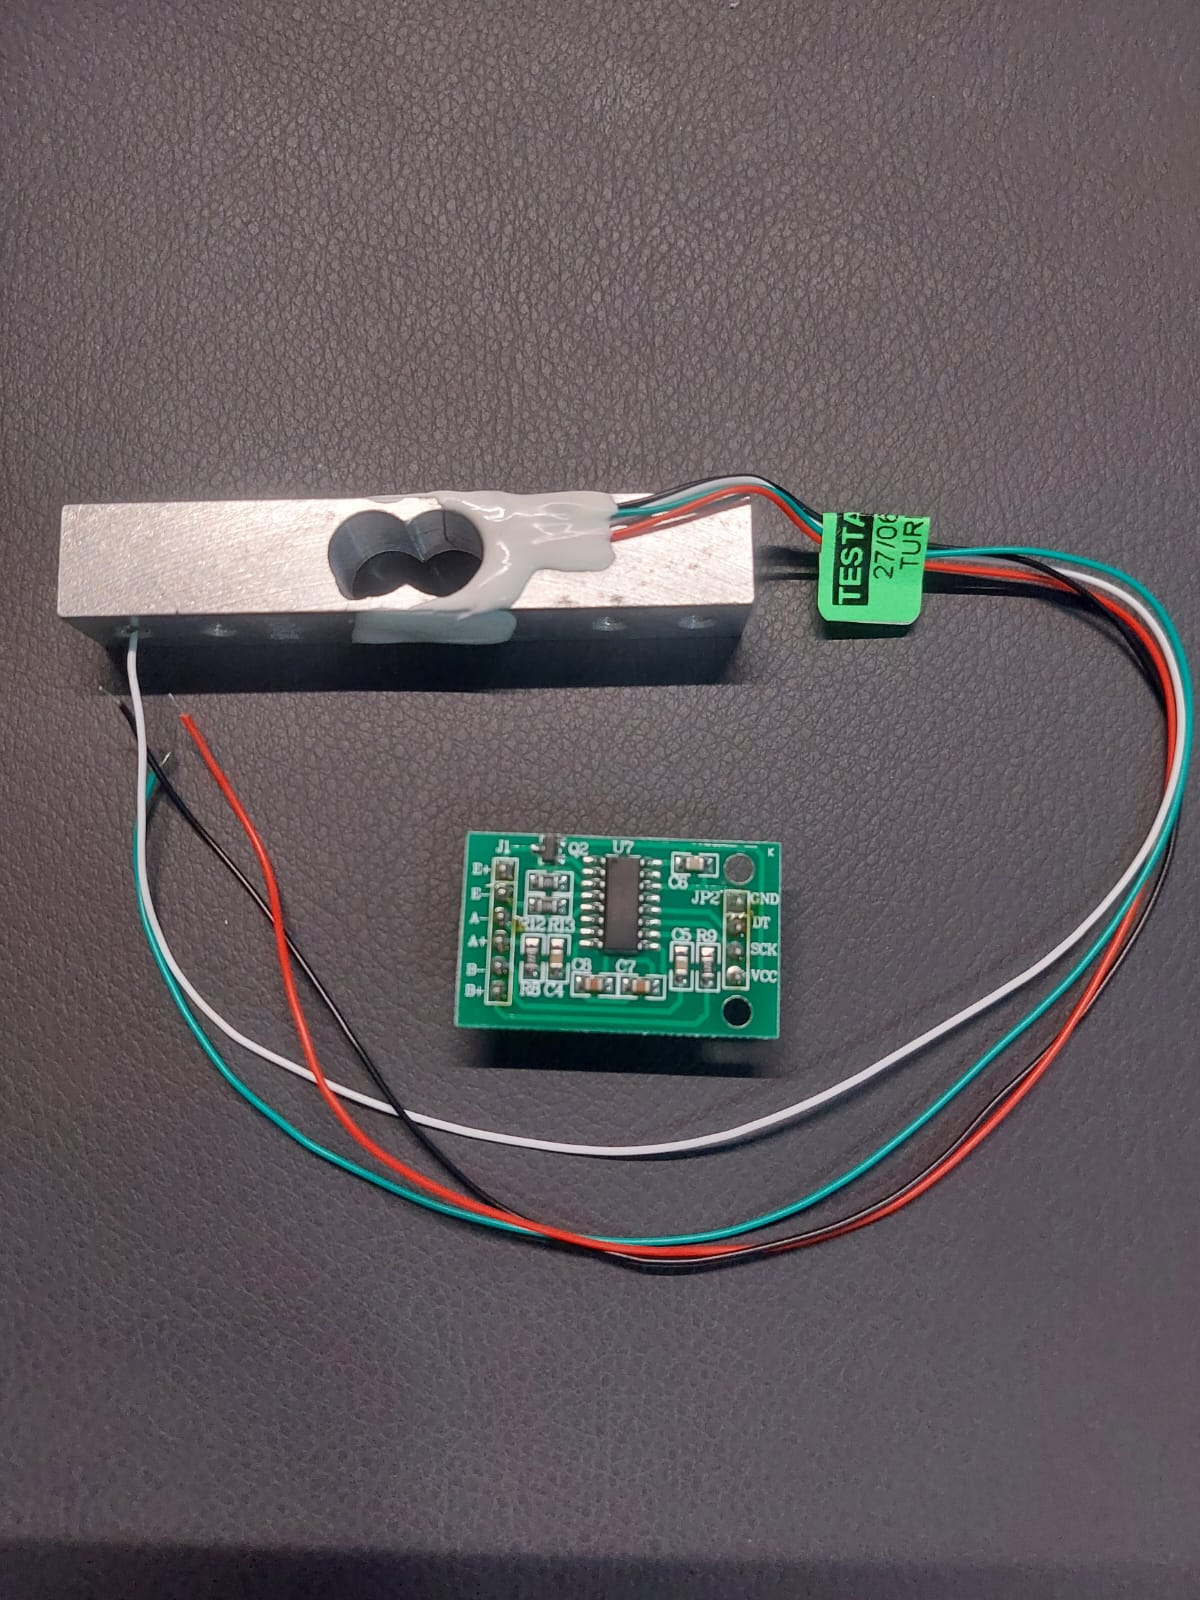
\includegraphics[width=0.4\textwidth]{./images/hx711.jpeg}
	\caption[HX711 breakout board and load cell]{HX711 breakout board and load cell}
	\fonte{}
	\label{fig:weighttesting}
\end{figure}

The HX711 integrated circuit comes in a breakout board, shown in Figure
\ref{fig:weighttesting}, that contains the necessary passive components and
includes the pin headers for connecting with other boards. The typical application 
circuit of the HX711 integrated circuit is shown in Figure \ref{fig:hx711circuit}.

\begin{figure}[H]
	\centering
	\caption[Typical HX711 circuit]{Typical HX711 circuit}
    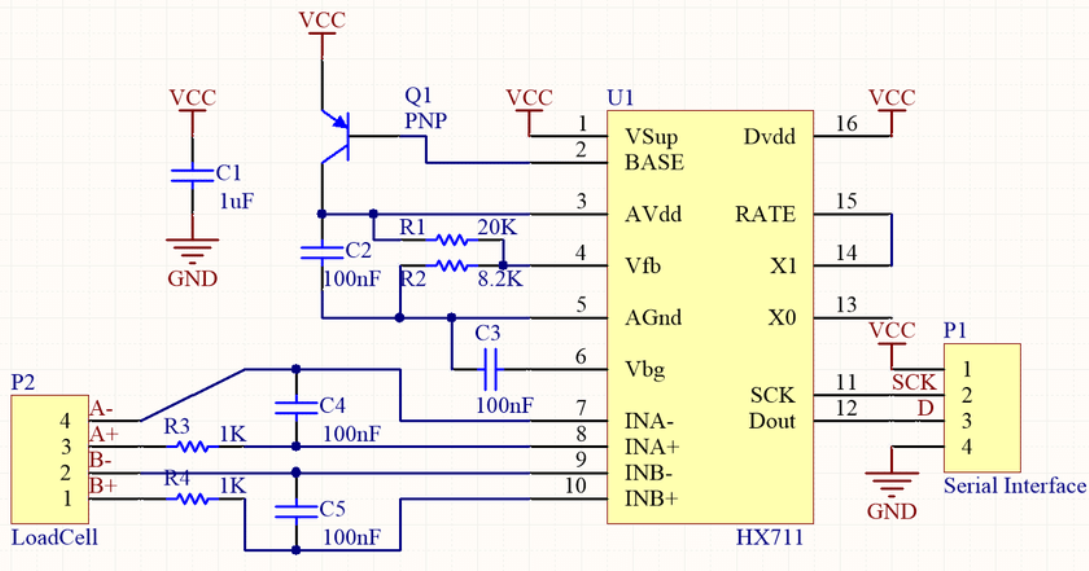
\includegraphics[width=0.8\textwidth]{./images/hx711circuit.png}
    \fonte{\cite{Ross2019}}
    \label{fig:hx711circuit}
\end{figure}

The Raspberry Pi board was connected to the HX711 through its GPIO pins,
allowing it to obtain the sensor readings through the serial interface. The
protocol used does not follow any known standard and can be
described as a \textit{Non-I2C compliant two-wire
protocol}\footnote{https://github.com/queuetue/Q2-HX711-Arduino-Library}.

An open-source driver implementation was used\footnote{https://github.com/tatobari/hx711py}, 
which included all the necessary features for the prototype.

As shown on Figure \ref{fig:devassembly}, the load cell requires a minimal
mechanical assembly to be tested properly, and for that two small wood plates
were used to secure the load cell and breakout board during development.

\begin{figure}[H]
	\centering
    \caption[Assembly used during development, including the Raspberry Pi, HX711 and load cell assembly]{Assembly used during development, including the Raspberry Pi, HX711 and load cell assembly}
    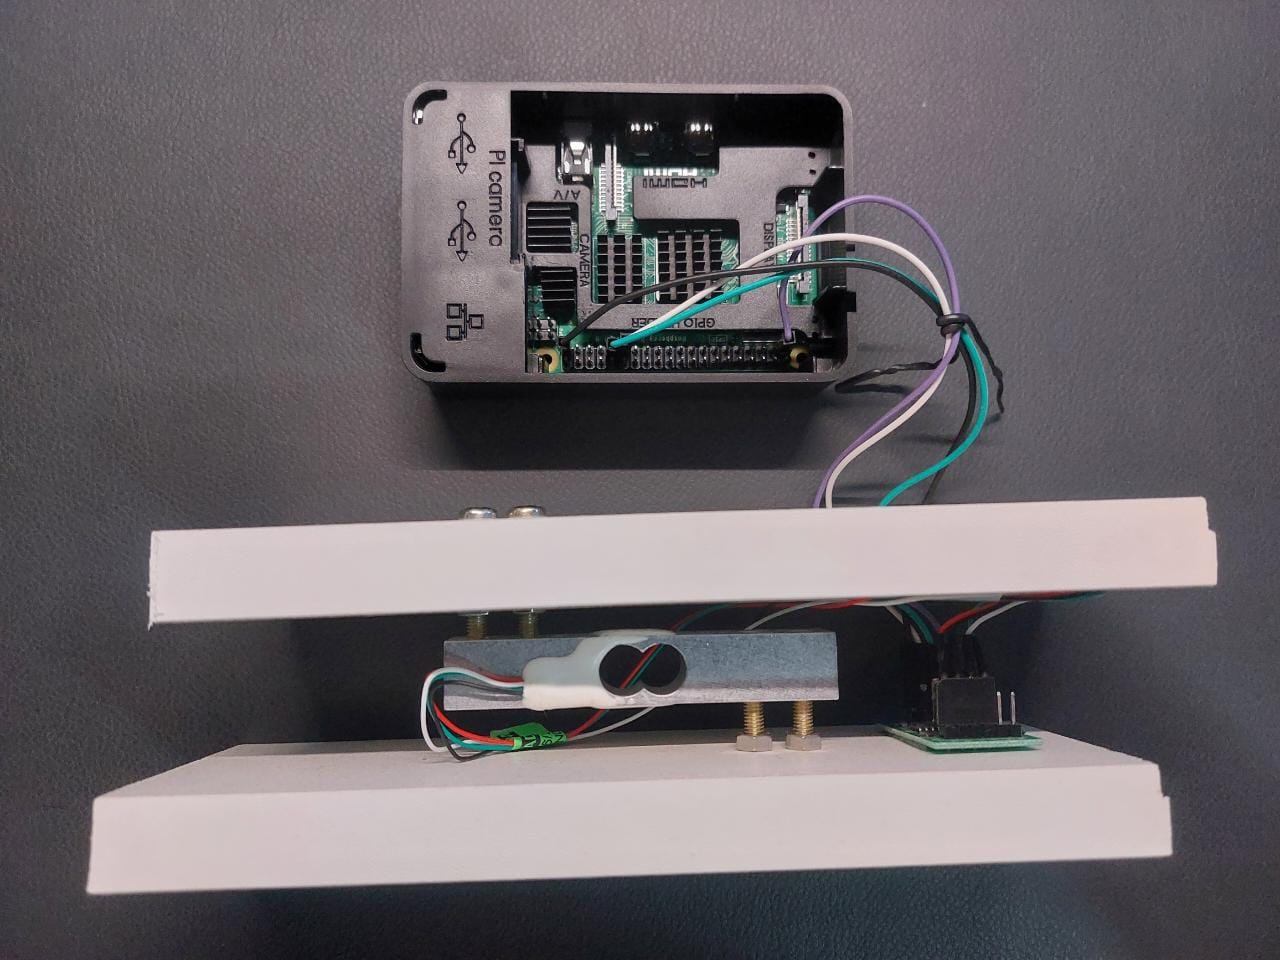
\includegraphics[width=0.7\textwidth]{./images/raspberrypiwithloadcell.jpeg}
	\fonte{}
	\label{fig:devassembly}
\end{figure}

\subsection{Camera}

In order to obtain a video feed to run object detection on, a camera system was
required. For that, a standard consumer webcam was used for its reduced cost
and good operating system driver support.

The webcam used was a Microsoft LifeCam
Cinema\footnote{https://www.microsoft.com/pt-BR/accessories/products/webcams/lifecam-cinema},
 shown in Figure \ref{fig:camera}, capable of capturing video in 720p up to 30\siglaPt{FPS}{Frames Per Second}, more
than enough for our prototyping requirements.

\begin{figure}[H]
	\centering
    \caption[Microsoft LifeCam Cinema Webcam used]{Microsoft LifeCam Cinema Webcam used}
    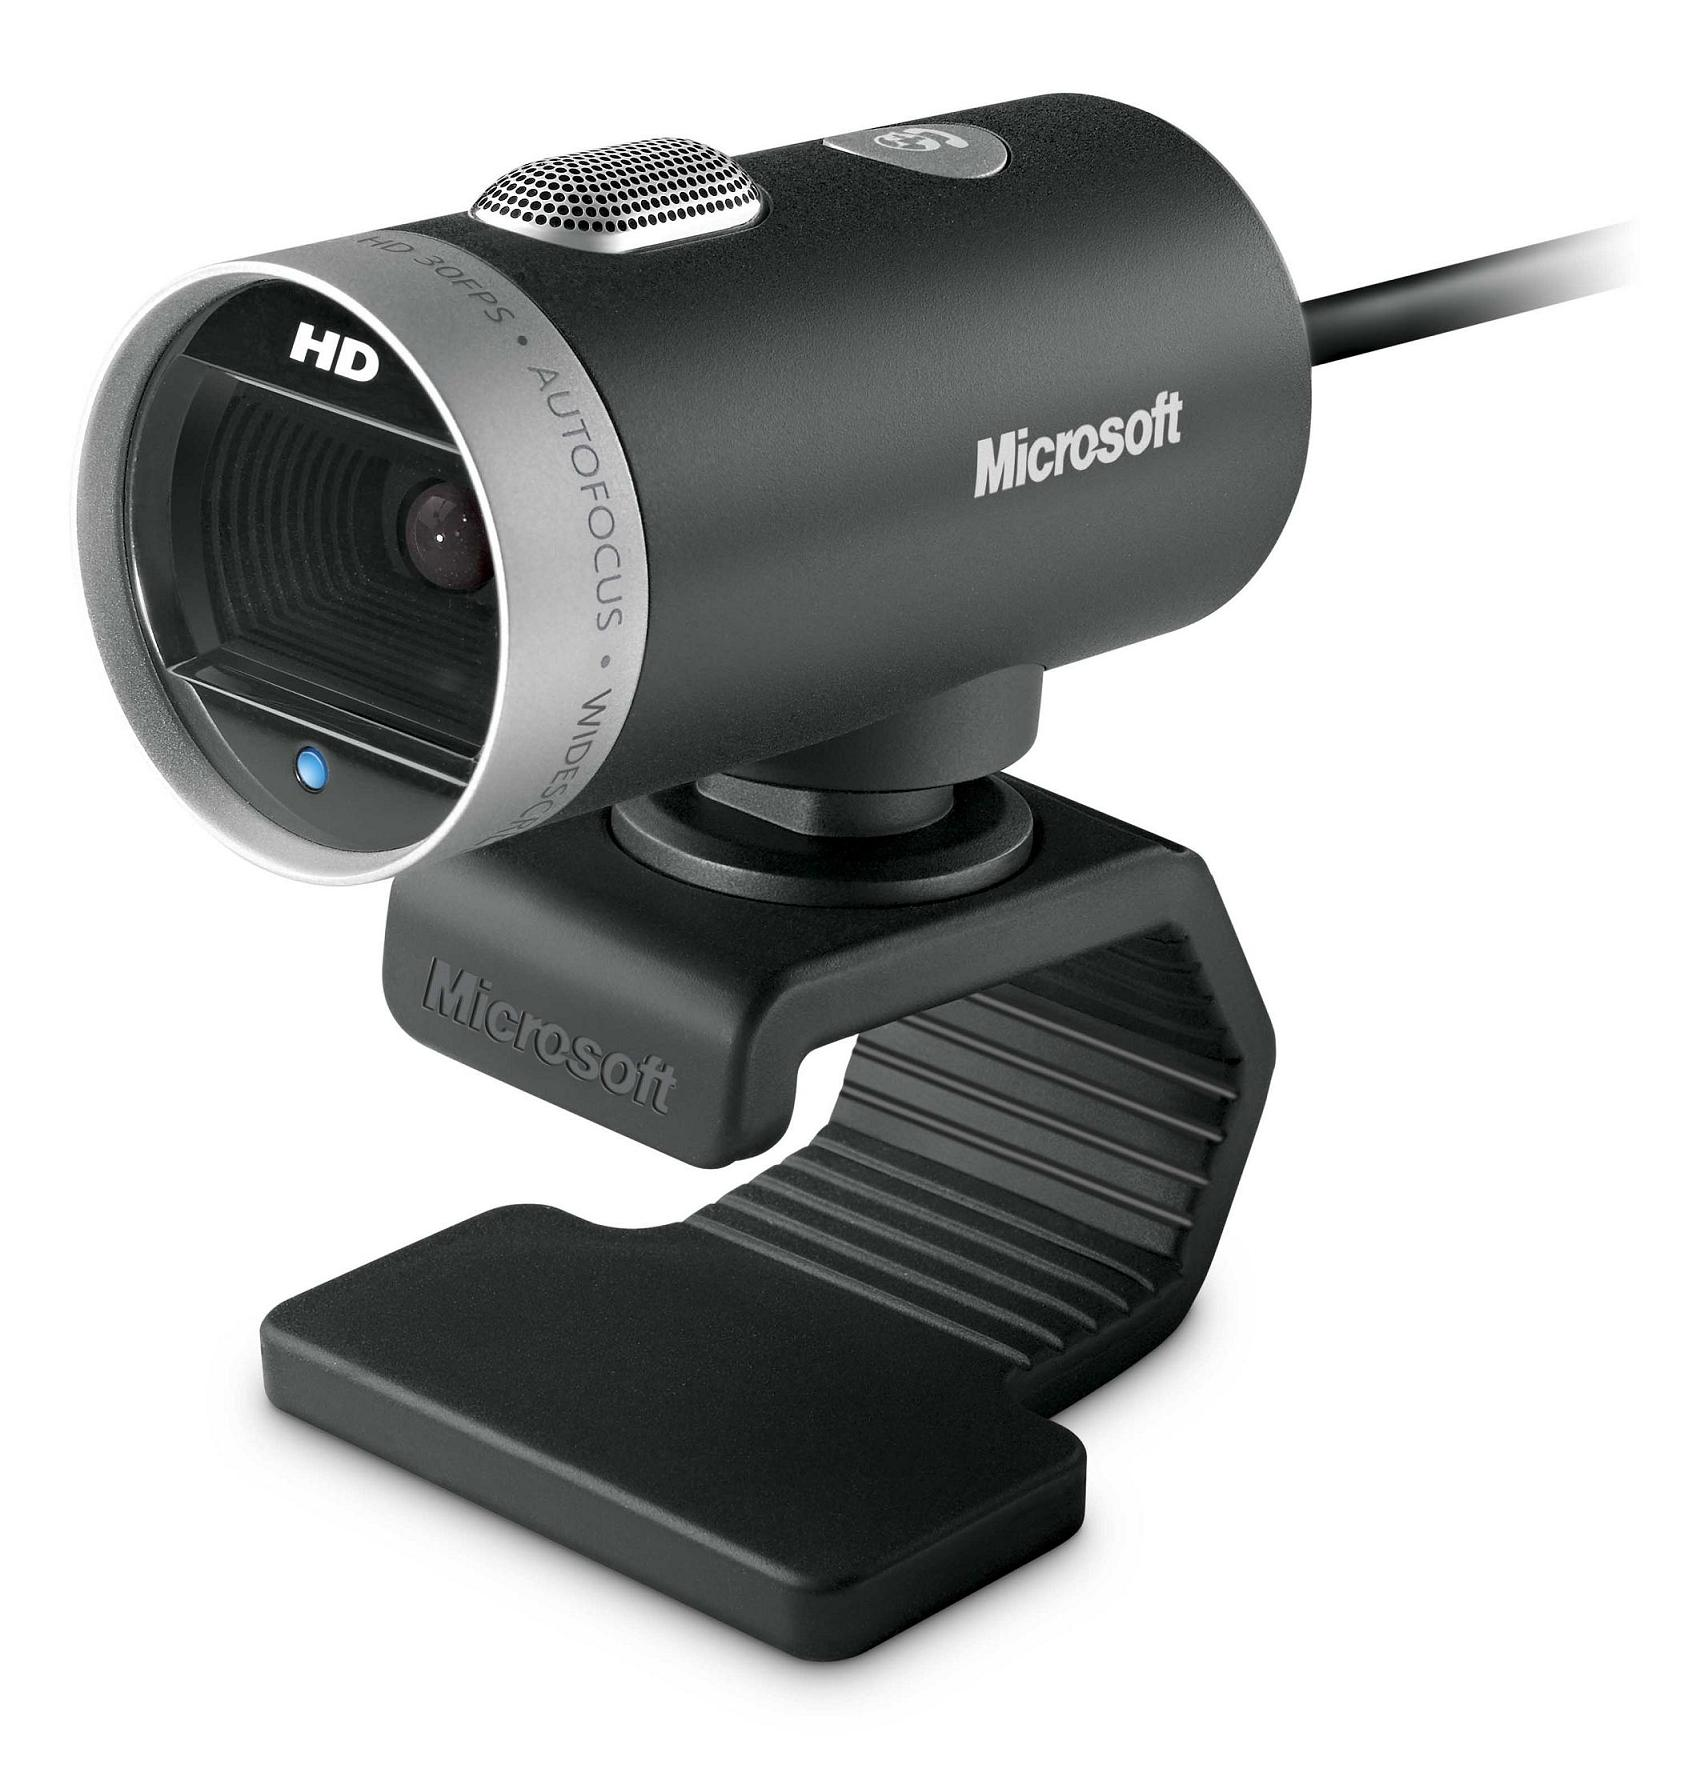
\includegraphics[width=0.3\textwidth]{./images/webcam.jpg}
	\fonte{}
    \label{fig:camera}
\end{figure}

\subsection{Application}

Developed in the Python\footnote{https://python.org} programming language, the
Product Recognizer application will provide the compute capabilities to apply
our business logic for processing the video feed provided by the camera and the
readings from the weight sensor.

The Python language was chosen for its vast tooling for working with computer
vision, sensors and interacting with the Raspberry Pi's built-in devices. The
language has also became a \textit{lingua franca} in the Machine Learning and
Data Science community as shown by volume of publications using it in the last
decade \cite{Wes2017,Joel2019,Andreas2016}.

The Product Recognizer application also uses a multi-threaded design to allow
concurrent processing, an important factor when considering the amount
\siglaPt{I/O}{Input/Output} operations performed.

Since Python's threading implementation does not allow for multiple threads to
execute in parallel -- i.e. at the same time -- a multi-process design could take
better advantage of the four available processing cores in the Raspberry Pi CPU
but that path was not explored and will be left for future iterations.

The three threads created are described below:
\begin{itemize}
    \item Frame Reader Thread: Responsible for reading frames from the Camera and making them available to the Main Thread.
    \item Main Thread: Responsible for bootstraping the application - including creating the other threads - and executing the main loop of
        object detection.
    \item Product Recognizer Thread: Responsible for applying the business logic using the objects detected and the weight sensor readings.
\end{itemize}

These threads communicate in synchronous and asynchronous means to achieve the overall goal of processing video and sensor data, as shown on Figure \ref{fig:threads}.

\begin{figure}[H]
	\centering
	\caption[Thread communication for the Product Recognizer Appplication]{Thread communication for the Product Recognizer Application}
    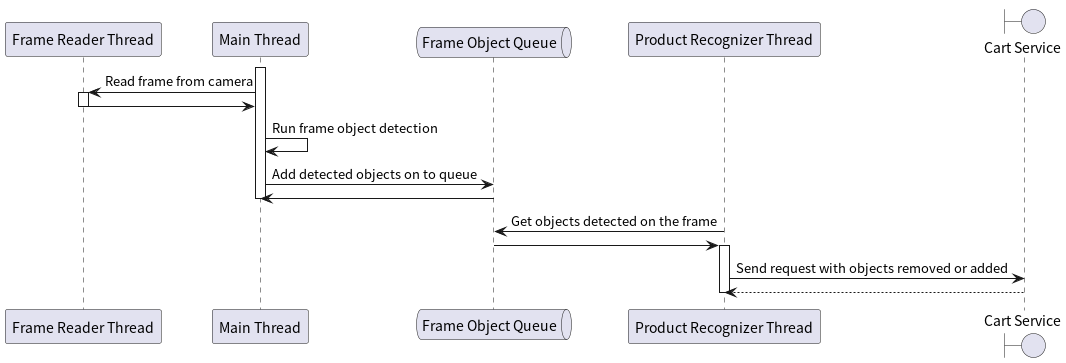
\includegraphics[width=1\textwidth]{./images/Product Recognizer Thread communication.png}
	\fonte{}
	\label{fig:threads}
\end{figure}

\begin{sourcecode}
\caption{Loop of the Main Thread. Some details were ommitted for the sake of brevity}
\begin{lstlisting}[language=Python,label={lst:main}]
while True:
  try:
    # Get frame from camera, provided by Frame Reader thread
    frame = stream.read_frame()

    # Preprocess and run object detection
    input = preprocessor.process(frame)
    detector.infer(input)

    # Filter objects by their class and confidence threshold
    objects = detector.get_objects()
    filtered_objects = object_filter.filter(objects)

    # Add filtered objects to the queue
    frame_objects_queue.put(filtered_objects)
\end{lstlisting}
\fonte{}
\end{sourcecode}

As shown on Listing \ref{lst:main} and in Figure \ref{fig:threads}, the Main
thread will do the computational work to fetch the frames from the camera that
were read by the Frame Reader thread, pre-process and run the object detection
model in it. The objects are then filtered and then added to a message queue
that will be used by the Product Recognizer thread to apply our product
detection rules.

\subsection{Product Recognizer Thread}

The Product Recognizer Thread is responsible for applying the main business
logic of detecting the addition and removal of products by leveraging the
objects detected in the frame and the readings provided by the weight sensor.

The thread will execute an infinite loop to constantly observe the objects
detected in the frame and the weight readings to detect product additions
and removals.

It uses two main variables to keep track of the current state:
\begin{itemize}
    \item A dictionary of which products are present in the cart and their count.
    \item The weight associated with the products present in the cart.
\end{itemize}

The first important step in the thread's logic is the \textit{Frame Diff}. This step 
calculates the difference in terms of the objects detected in the current 
and previous frames (e.g. whether objects were added, removed, or remain the same) 
and store it in a dictionary data structure\footnote{https://docs.python.org/3/tutorial/datastructures.html\#dictionaries},
by comparing the stored product dictionary and the received list of frame
objects from the Main Thread.

\begin{figure}[H]
	\centering
	\caption[Illustration of the frame diff'ing scheme]{Illustration of the frame diff'ing scheme. A can was added on frame $n+1$ and therefore will generate a diff of one can. If the reading from the weight sensor matches the expected one, the product will be added to the cart.}
    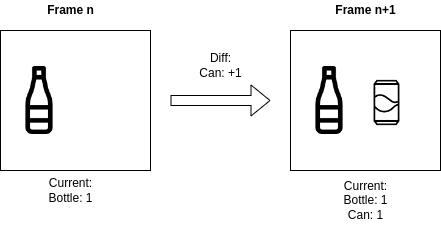
\includegraphics[width=0.8\textwidth]{./images/diagrams/framediff.png}
	\fonte{}
    \label{fig:diff}
\end{figure}

Given the frame object diff, it is then possible to calculate an expected
weight change based on the weight of each item - and their quantity - contained
in the diff. The expected weight difference is then compared to the actual
one obtained from the weight sensor, considering a configurable tolerance.

In this scenario, the weight readings are used as a filter and act as a
\textit{commit} step for differences detected in the frame objects. This way, objects are not
added or removed from the cart simply by appearing or disappearing from the frame.

In the example show in Figure \ref{fig:diff}, if the illustrated can weights an expected 400 grams, the weight
difference expected should be close to 400 grams. If the weight difference does not match the expected
one, the object will not be considered for addition or removal. 

A more detailed activity diagram of the logic executed in the Product Recognizer thread loop is
shown in Figure \ref{fig:activity}.

\begin{figure}[H]
	\centering
	\caption[Activity diagram for the Product Recognizer thread]{Activity diagram for the Product Recognizer thread}
    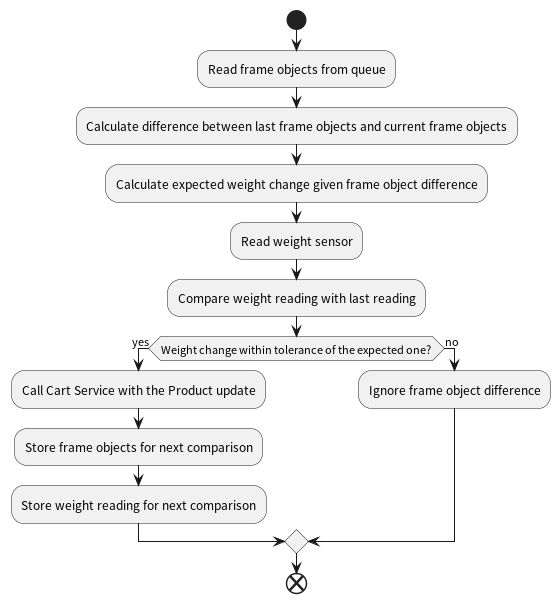
\includegraphics[width=0.8\textwidth]{./images/Product Recognizer Activity.png}
	\fonte{}
    \label{fig:activity}
\end{figure}

\begin{sourcecode}
\caption{Product Recognizer thread logic}
\begin{lstlisting}[language=Python]
objects = self.queue.get_nowait()

# Preprocessing step just to format data
current_frame_objects = self.__build_object_dict(objects)

# Calculate the frame diff using the last and current frame objects
frame_diff = self.__get_frame_diff(
    current_frame_objects, self.last_frame_objects
)

if len(frame_diff) == 0:
    self.log.info("empty diff")
    continue

# Get current weight reading
weight_reading = self.weight_sensor.get_reading(samples=5)

for label, count in frame_diff.items():
    if not self.__valid_weight_difference(label, count, weight_reading):
        self.log.info("ignoring, not valid weight difference")
        continue

    # Send request to cart service
    self.__call_cart_service(label, count)

    # Update stored state
    self.last_weight_reading = weight_reading
    self.last_frame_objects[label] = current_frame_objects[label]
    if self.last_frame_objects[label] == 0:
        del self.last_frame_objects[label]
\end{lstlisting}
\fonte{}
\end{sourcecode}

\subsection{Object Detection Model}

The code used to train our Object Detection models was made available in GitHub,
in our Project's Repository
\footnote{https://github.com/fsmiamoto/zcart/blob/master/product\_recognizer/model/notebooks/}.
It can be used for reference and for performing a further deep dive into this section.

Five products were chosen for the purpose of setting up and demonstrating the Object Recognition 
capability of our product: a Blue Pens Packet; a Card Deck; a Coke Can; a Guarana Soda Can; 
and a Post It Pack. 
The data used for training our custom Object Detection model was collected and labelled by us
using Edge Impulse\footnote{https://www.edgeimpulse.com/}, a development platform for Machine 
Learning on Edge devices.
A total of \textbf{1000 photos} were taken using the Data Collection feature of
the Edge Impulse Studio, shown in Figure \ref{fig:edgeimpulse1}, using the same
webcam that is used for the inference in our final product. Our photos included
images showing each one of the products in different scenarios and positions,
and also images where more than one product was present.

\begin{figure}[H]
	\centering
	\caption[Collecting Data in Edge Impulse]{Collecting Data in Edge Impulse}
    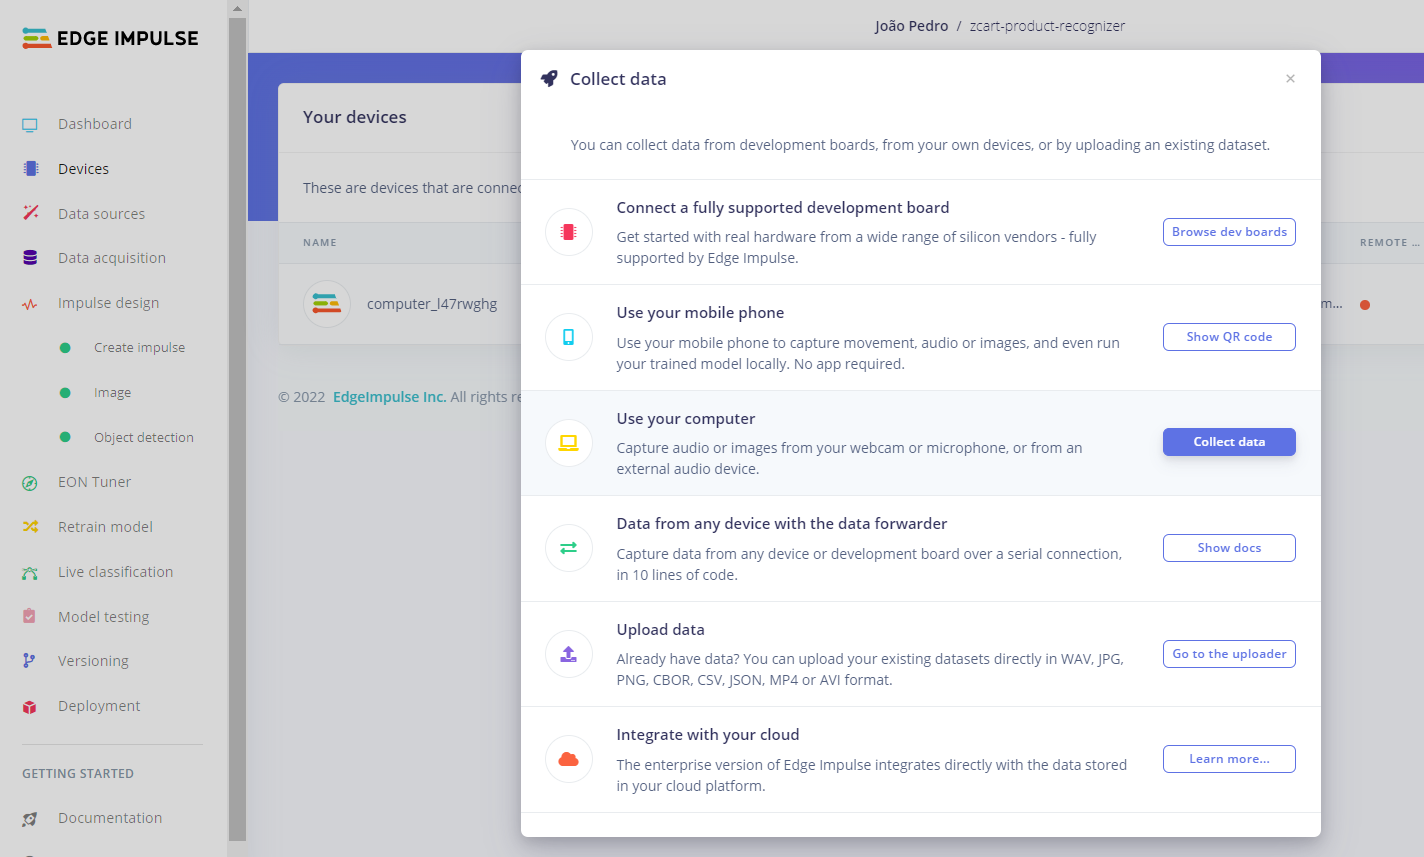
\includegraphics[width=0.8\textwidth]{./images/edge-impulse-collect-data.png}
	\fonte{Edge Impulse (2022)}
    \label{fig:edgeimpulse1}
\end{figure}

The pictures were then were labeled using the Labeling
Queue\footnote{https://docs.edgeimpulse.com/docs/edge-impulse-studio/data-acquisition/labeling-queue}
feature of Edge Impulse, which allowed us to draw Bounding Boxes around the
desired objects for detection, as shown in Figure \ref{fig:edgeimpulse2}.

\begin{figure}[H]
	\centering
	\caption[Labelling Queue in Edge Impulse]{Labeling Queue in Edge Impulse}
    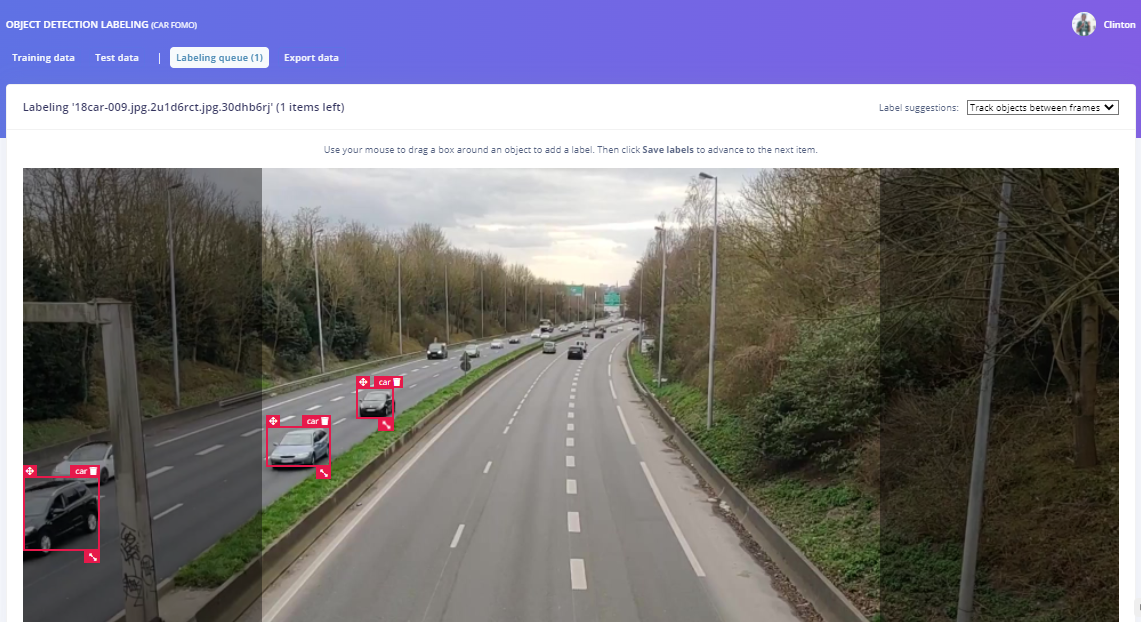
\includegraphics[width=0.9\textwidth]{./images/edge-impulse-labelling-queue.png}
	\fonte{Edge Impulse (2022)}
    \label{fig:edgeimpulse2}
\end{figure}

The raw pictures and bounding boxes were then exported from Edge Impulse such
that we could pre-process the data and model our custom object detection
algorithm using the Python programming language. The pictures were exported in
their raw JPEG\footnote{Defined in ISO/IEC 10918}  file format, comprised in a
ZIP folder. The bounding boxes were exported in the format of a JSON file
containing the coordinates for the boundaries and the metrics for each picture,
allowing us to easily reconstruct the bounding boxes for each object in each
image using programming instructions. The files were then loaded to a Cloud
Object Storage Bucket in AWS \footnote{https://aws.amazon.com/}, making it
easier for us to access the data by importing it from the web using any
programming language.

Listing \ref{lst:boundingBoxCoordinates} shows a section of an example JSON file containing
the bounding boxes.

\begin{sourcecode}
\caption{Bounding boxes coordinates file exported from Edge Impulse}
\begin{lstlisting}[label={lst:boundingBoxCoordinates}]
	{
		"version": 1,
		"type": "bounding-box-labels",
		"boundingBoxes": {
		  "im1.jpg": [
			{
			  "label": "blue_pens",
			  "x": 120,
			  "y": 265,
			  "width": 172,
			  "height": 207
			},
			{
			  "label": "card_deck",
			  "x": 285,
			  "y": 120,
			  "width": 136,
			  "height": 247
			}
		  ],
		  "im2.jpg": [
			(...)
		  ]
		}
	}
\end{lstlisting}
\fonte{}
\end{sourcecode}

The development environment used for writing the code for training our custom
model was Google Colab\footnote{https://colab.research.google.com/}, and the
programming language of choice was Python. Google Colab consists on a web-based
interface, shown in Figure \ref{fig:googlecollab}, that allows developers to
use Google's infrastructure (with GPUs and TPUs) for writing and executing
code.

\begin{figure}[H]
	\centering
	\caption[Google Colab - Overview of Colaboratory Features]{Google Colab - Overview of Colaboratory Features}
    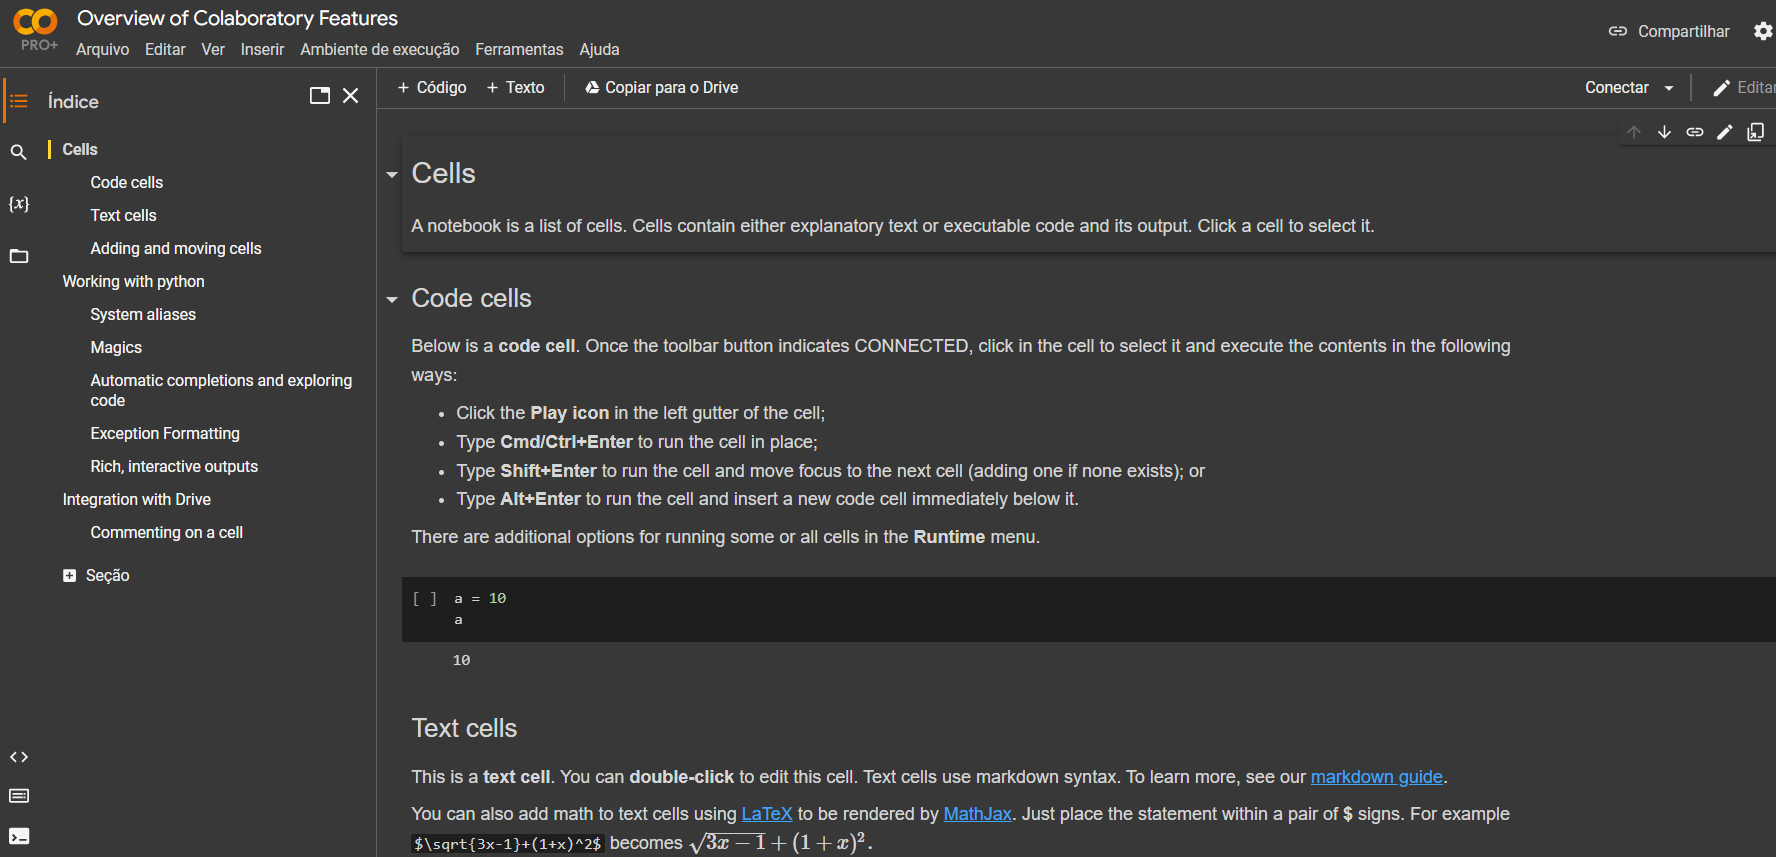
\includegraphics[width=1\textwidth]{./images/google-colab.png}
	\fonte{Google\footnote{https://colab.research.google.com/notebooks/basic\_features\_overview.ipynb}}
    \label{fig:googlecollab}
\end{figure}

The Edge Impulse files were loaded from our cloud object storage bucket, and then manipulated in Python
from Google Collab such that we could utilize the images and bounding box coordinates for training
our model.

We decided to use Google's TensorFlow\footnote{https://www.tensorflow.org/} framework to train our 
models, as it is one of the most popular frameworks employed in the Industry for training AI models
and also because it features a lightweight library called TensorFlow Lite\footnote{https://www.tensorflow.org/lite}, 
which is appropriate for creating efficient edge and mobile AI models considering the 
typical hardware constraints from these types of devices.

To train our model, we used the TensorFlow Lite's ModelMaker API\footnote{https://www.tensorflow.org/lite/models/modify/model\_maker} 
for Object Detection, which simplifies the process of training our models by breaking down the most
complex concepts of deep learning into parameterized objects and methods, allowing us to spend
more time on the pre-processing steps and on experimenting with different network configurations
to improve the model's accuracy. 

As of writing this work, the ModelMaker API only has compatibility
with the EfficientDet family of architectures \cite{Mingxing2020} for training
Deep Learning models for Object Detection. The EfficientDet family is efficient
for object recognition in edge devices, altough contemporany architectures,
such as the YOLOv5 and its successors, can have better performance, as shown in Figure \ref{fig:yoloefficientdet}.

\begin{figure}[H]
	\centering
	\caption[YOLOv5 vs EfficientDet - Performance Comparison]{YOLOv5 vs EfficientDet - Performance Comparison}
    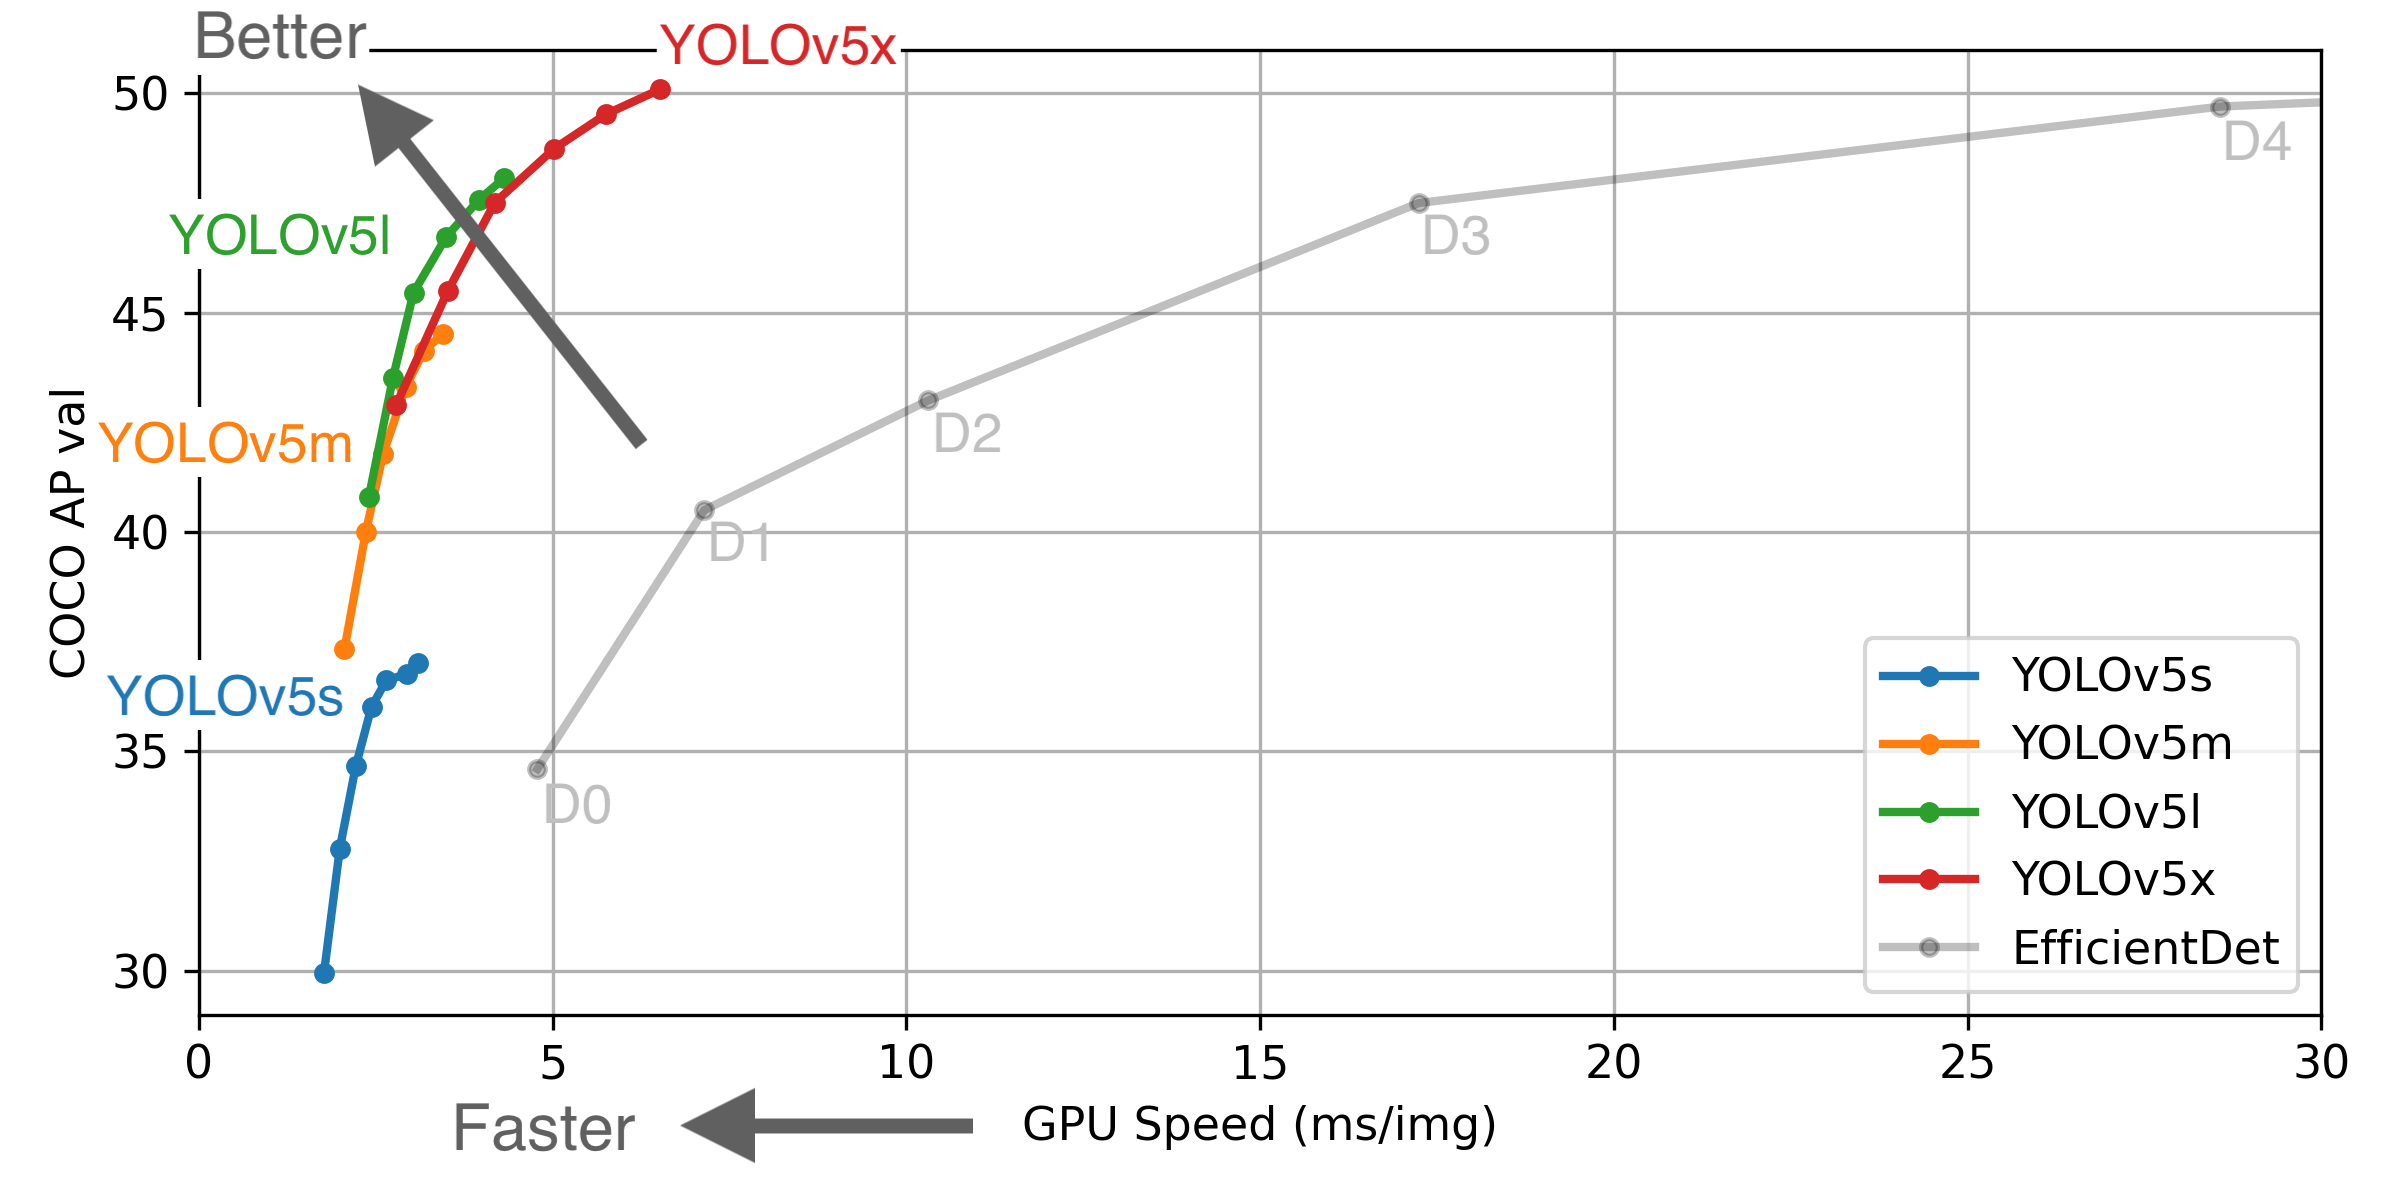
\includegraphics[width=0.9\textwidth]{./images/yolo-efficientdet-comparison.png}
	\fonte{YOLOv5 Release Notes\footnote{https://github.com/ultralytics/yolov5/releases/tag/v4.0}}
    \label{fig:yoloefficientdet}
\end{figure}

Our initial plan was to use the YOLOv5 architecture, but since its
implementation is not native to TensorFlow Lite, it would require us to create
additional wrappers around the outputs of the YOLOv5 network to get it working
as expected. Even thought it is possible to convert the models from their
original PyTorch\footnote{https://pytorch.org/} format to a TensorFlow Lite
format, the conversion does not cover some of the features from the original
implementation\footnote{https://github.com/ultralytics/yolov5/issues/1981},
which limits its direct functionality. Similar compatibility issues happen with
the latest YOLO implementations, such as the
YOLOv7\footnote{https://medium.com/geekculture/journey-putting-yolo-v7-model-into-tensorflow-lite-object-detection-api-model-running-on-android-e3f746a02fc4}.
Thus, we have decided to proceed with the TensorFlow Lite's Model Maker API
compatible architectures -- namely the EfficientDet family --  since it would
have taken a considerable time to troubleshoot conversion defects from the YOLO
architecture and all that work would not bring any additional value to our
prototype.

Since our original images were saved in the 640x480 resolution and the expected
input of the EfficientDet network is of 320x320 px, two pre-processing
approaches were tried out for the training dataset: resizing and cropping the
images. The bounding box coordinates and dimensions were also adjusted
accordingly such that the data integrity was preserved. Figure
\ref{fig:preprocess} illustrates both of the approaches used.

\begin{figure}[H]
	\centering
	\caption[Image Preprocessing Strategies]{Image Preprocessing Strategies}
    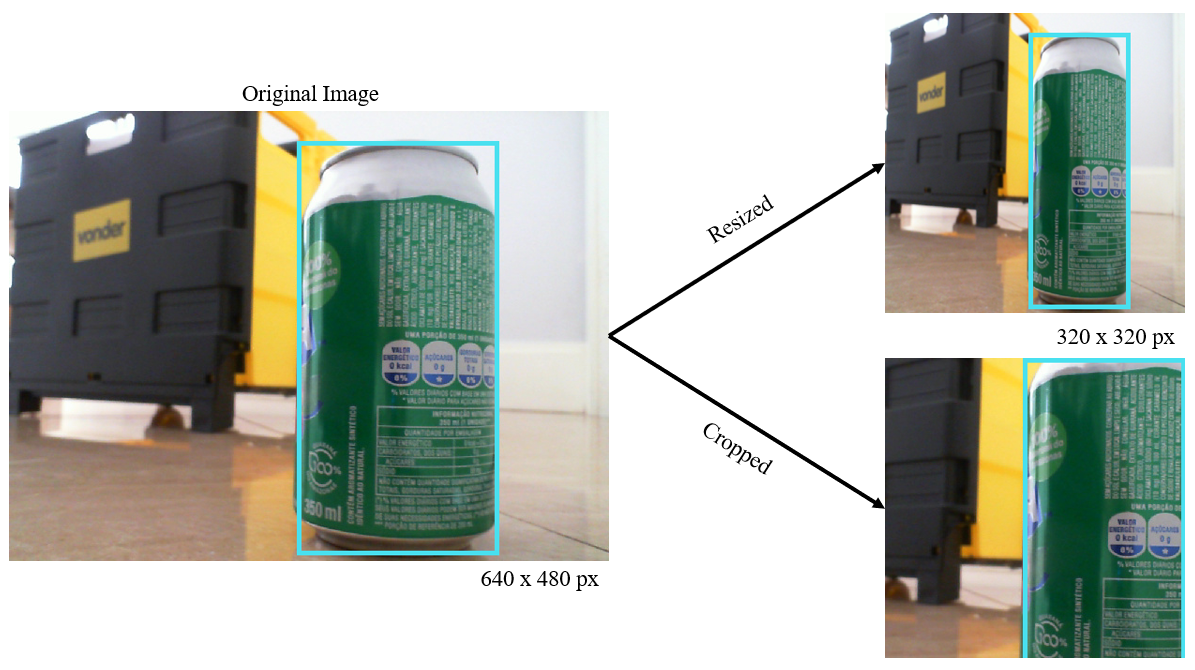
\includegraphics[width=1\textwidth]{./images/image_preprocessing.png}
	\fonte{}
    \label{fig:preprocess}
\end{figure}

Once the images and bounding boxes were pre-processed, the images were split
into Train, Validation and Test sets; and saved in the standardized format
required by the TensorFlow Lite's Model Maker for Object Detection API for
training, which consists of a Comma Separated Values (\siglaPt{CSV}{Comma
Separated Values}) file with the structure shown in Listing \ref{lst:csvFormatTrain}.

\begin{sourcecode}
\caption{CSV format for specifying the Train, Test and Validation 
	image sets for training models using the TensorFlow's Model Maker API for Object 
	Detection}
\begin{lstlisting}[label={lst:csvFormatTrain}]
Template:
set,path,label,x_min,y_min,,,x_max,y_max,,
set,path,label,x_min,y_min,x_max,y_min,x_max,y_max,x_min,y_max

Examples:
TEST,./images_path/im3.png,0.5,0.6,,,0.2,0.9,,
VALIDATION,./images_path/im4.png,coke_soda,0.3,0.4,,,0.4,0.8,,
TRAIN,./images_path/im5.png,guarana_soda,0.3,0.3,0.8,0.8,1.0,0.9,0.1,1.0
TRAIN,./images_path/im5.png,post_it,0.3,0.1,,,0.3,0.4,,
\end{lstlisting}
\fonte{}
\end{sourcecode}

Approximately 70\% of the photos shot were moved to the Train set, which is the set used for effectively 
tuning the weights and biases of the custom models; About 21\% were moved to the Validation set, 
being used to understand our model's performance under different training scenarios and steps; 
and the rest was used for testing the custom model after it was trained, which allowed us to 
get unbiased metrics on how it would approximately perform in real life \cite{MluExplain}.

Table \ref{tbl:imageSetsTab} describes the data sets created for training and evaluation in greater detail.

\begin{table}[H]
	\centering
	\caption[Image Sets Created for Training, Validation and Testing]{Image Sets Created for Training, Validation and Testing}
	\begin{adjustbox}{width=1\textwidth}
	\label{tab:imageSets}
	\begin{tabular}{c|c|c|c|c}
		\hline 
		Class & Number of Pictures & Pictures in the Train Set & Pictures in the Validation Set & Pictures in the Test Set \\
		\hline
        Blue Pens Packet & 293 & 206 & 61 & 26\\
		Card Deck & 306 & 215 & 64 & 27\\
		Coke Can & 276 & 194 & 58 & 24\\
		Guarana Soda Can & 283 & 199 & 59 & 25\\
		Post It Pack & 273 & 192 & 57 & 24\\
		\hline 
	\end{tabular}
	\end{adjustbox}
	\label{tbl:imageSetsTab}
	\fonte{}
\end{table}

Finally, we defined a programming loop to train different models using the EfficientDet-D0,
EfficientDet-D1, EfficientDet-D2, EfficientDet-D3 and EfficientDet-D4 architectures; both by
applying Transfer Learning on the top of pre-trained weights from training with the COCO-2017 dataset 
\footnote{https://cocodataset.org/\#home} and by training the entire networks based in our custom data. 

We ran this entire loop using the cropped images first; and then executed it using resized images with the EfficientDet-D0,
EfficientDet-D1 and EfficientDet-D2 architectures too, as they were the ones who offered better
performance balance considering our hardware constraints. 
With that, we came to have 16 distinct custom models for experimenting, as shown in Table \ref{tbl:modelsTrainedTab}.

\begin{table}[H]
	\centering
	\caption[Models Trained]{Models Trained}
	\begin{adjustbox}{width=1\textwidth}
	\label{tab:modelsTrained}
	\begin{tabular}{c|c|c|c}
		\hline 
		Model & Image Pre-Processing Strategy & Architecture & Whole Trained/Transfer Learning \\
		\hline
        1 & Cropping & EfficientDet-D0 & Whole Trained \\
		2 & Cropping & EfficientDet-D1 & Whole Trained \\
		3 & Cropping & EfficientDet-D2 & Whole Trained \\
		4 & Cropping & EfficientDet-D3 & Whole Trained \\
		5 & Cropping & EfficientDet-D4 & Whole Trained \\
		6 & Cropping & EfficientDet-D0 & Transfer Learning on COCO-2017 \\
		7 & Cropping & EfficientDet-D1 & Transfer Learning on COCO-2017 \\
		8 & Cropping & EfficientDet-D2 & Transfer Learning on COCO-2017 \\
		9 & Cropping & EfficientDet-D3 & Transfer Learning on COCO-2017 \\
		10 & Cropping & EfficientDet-D4 & Transfer Learning on COCO-2017 \\
		11 & Cropping & EfficientDet-D0 & Whole Trained \\
		12 & Cropping & EfficientDet-D1 & Whole Trained \\
		13 & Resizing & EfficientDet-D2 & Whole Trained \\
		14 & Resizing & EfficientDet-D0 & Transfer Learning on COCO-2017 \\
		15 & Resizing & EfficientDet-D1 & Transfer Learning on COCO-2017 \\
		16 & Resizing & EfficientDet-D2 & Transfer Learning on COCO-2017 \\
		\hline 
	\end{tabular}
	\end{adjustbox}
	\label{tbl:modelsTrainedTab}
	\fonte{}
\end{table}

\section{Mechanical Assembly}

A foldable utility cart was selected as a core
component with two additional wood plates, used for creating a \textit{false
bottom} shown in Figure \ref{fig:falsebottom}. Between the plates, the load cell and Raspberry Pi board were secured
in place using bolts, screws and velcro.

Figures \ref{fig:prototype1} and \ref{fig:prototype2} show an overview of the structure built.

\begin{figure}[H]
	\centering
	\caption[Overall mechanical assembly including the LCD and Camera]{Overall mechanical assembly including the LCD and Camera}
    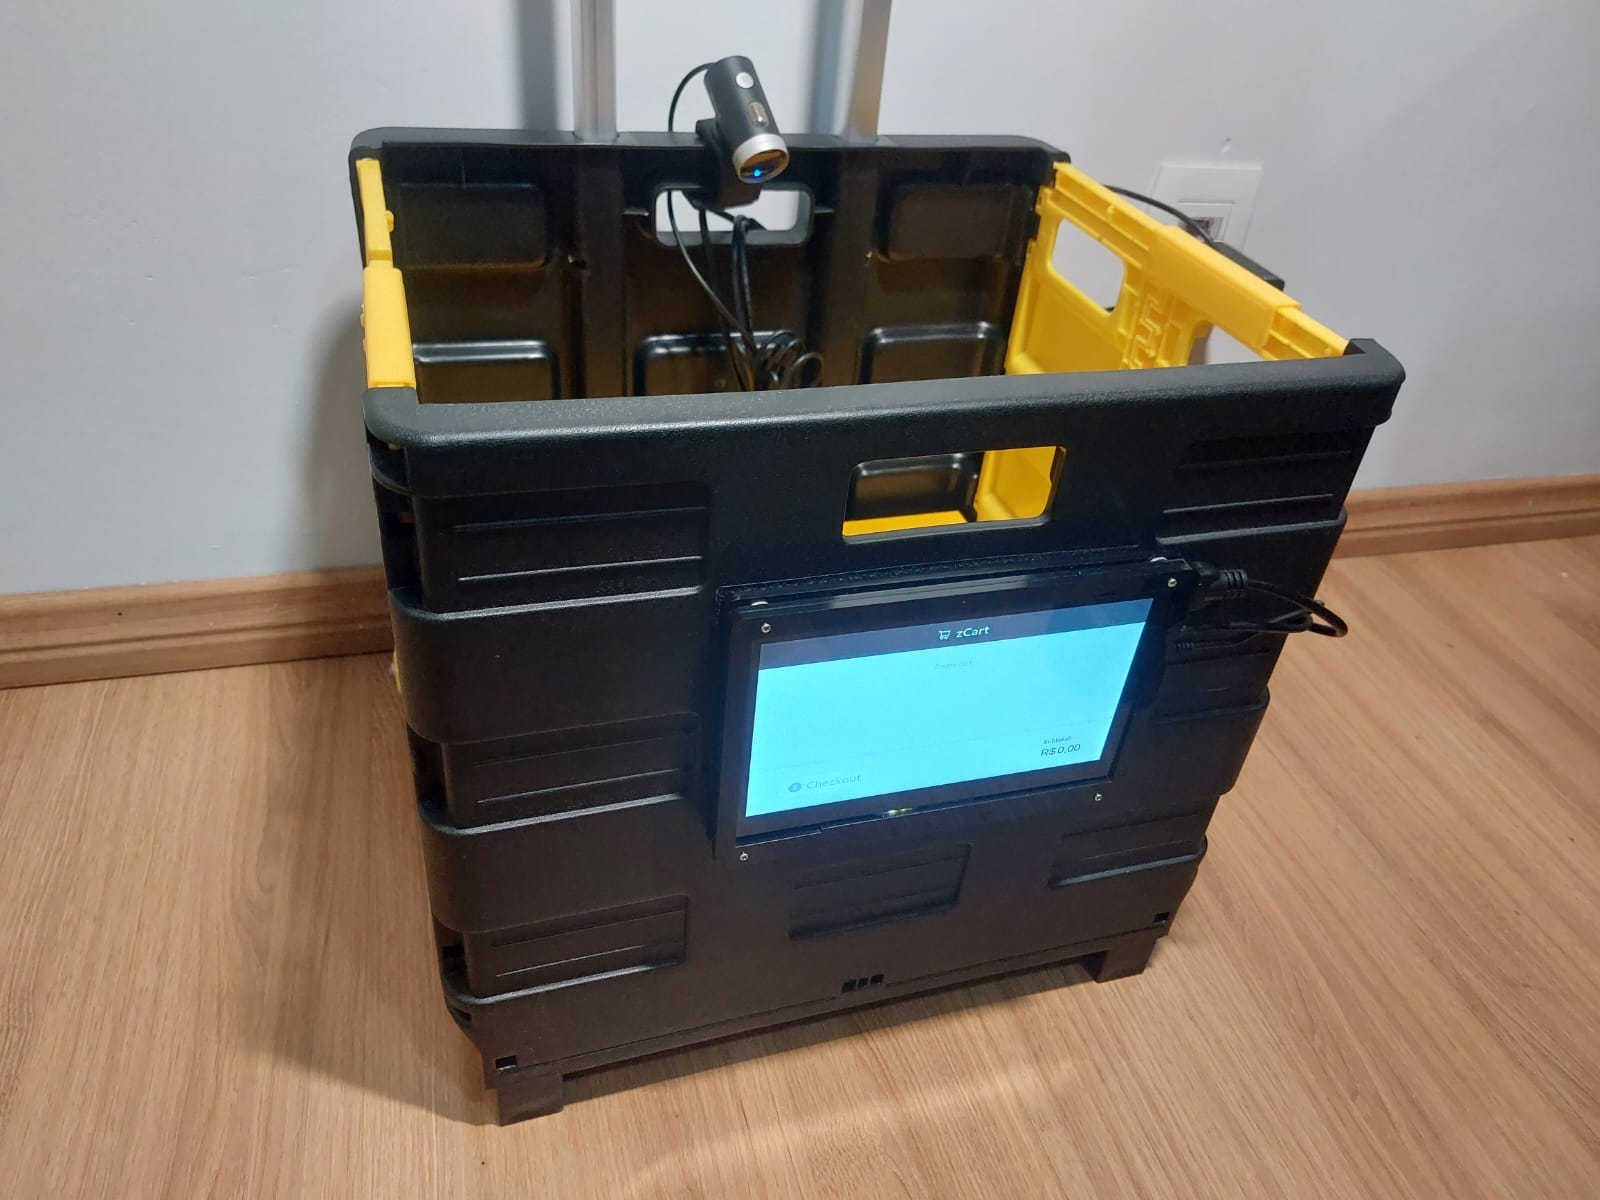
\includegraphics[width=0.75\textwidth]{./images/cart.jpeg}
	\fonte{}
    \label{fig:prototype1}
\end{figure}

\begin{figure}[H]
	\centering
	\caption[Top view of the assembly showing the false bottom]{Top view of the assembly showing the false bottom}
    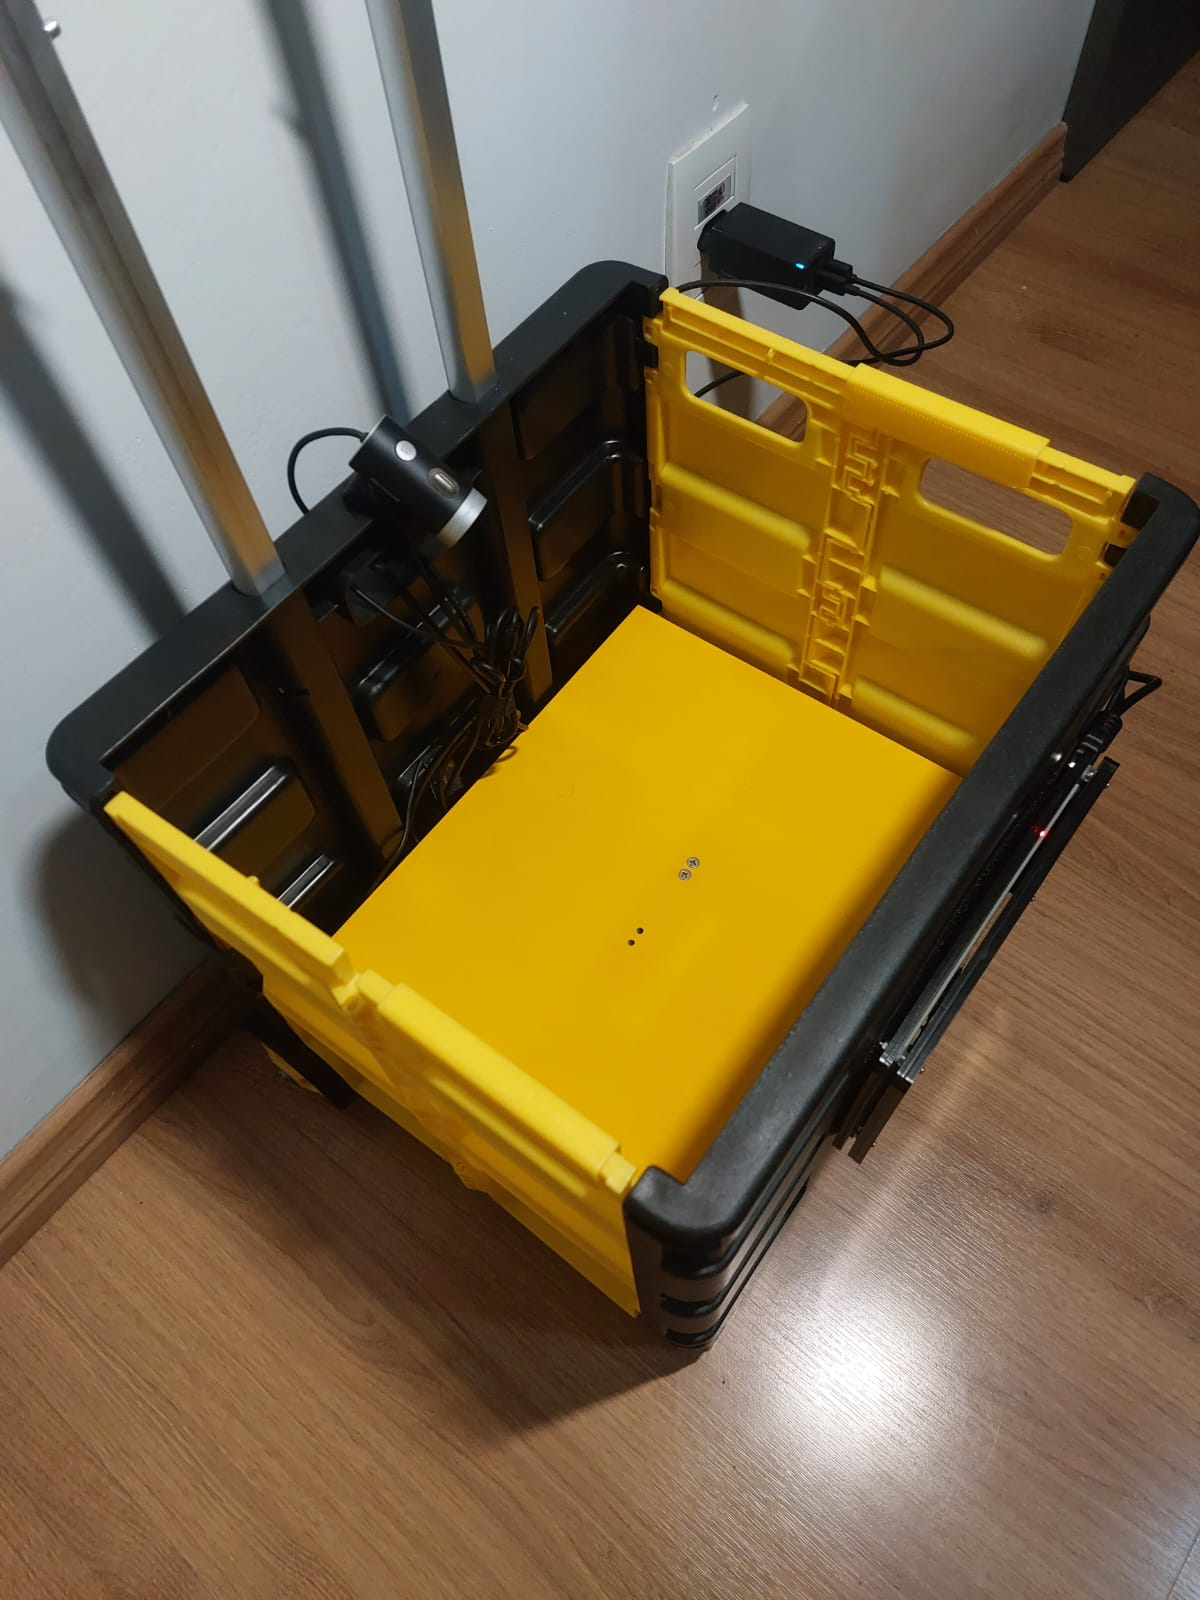
\includegraphics[width=0.5\textwidth]{./images/carttop.jpeg}
	\fonte{}
    \label{fig:prototype2}
\end{figure}

Considering the objectives of the prototype, the shape of the mechanical
housing was not considered to be of great relevance and using a real
supermarket cart would have been impractical considering its size and cost. Still, we wanted
to keep a shape that would represent the overall idea of a smart cart.

\begin{figure}[H]
	\centering
	\caption[False bottom structure with the load cell and Raspberry Pi board in between]{False bottom structure with the load cell and Raspberry Pi board in between}
    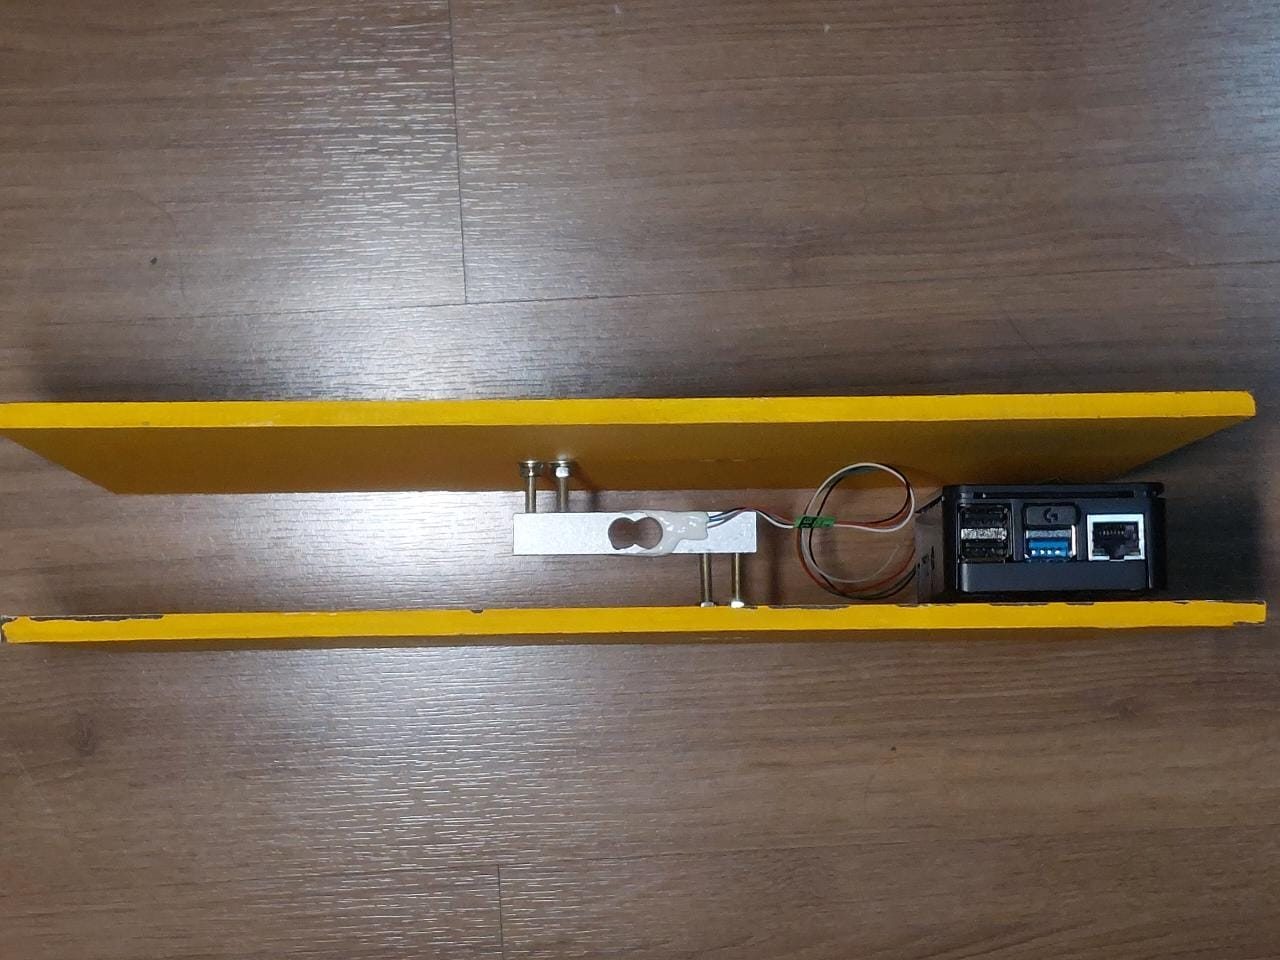
\includegraphics[width=0.6\textwidth]{./images/cartbase2.jpeg}
	\fonte{}
    \label{fig:falsebottom}
\end{figure}

Additional photos of the prototype can be seen on Appendix \ref{app:photos}.
%% Comente para remover este item

%% Capítulo
%%%% CAPÍTULO 4 - RESULTADOS E DISCUSSuO

\chapter{Results}\label{cap:resultados}

\section{Model Accuracy}

The most lightweight models were the preferred ones considering our edge device capabilities,
as they offer better inference time performance. 
However, we were also looking for the most optimal accuracy and loss metrics, 
therefore the models were evaluated with test images, which were never introduced to the models
during training, to make sure that they were efficient on the what they are ultimately supposed to do, 
which is to detect products.

Figures \ref{fig:singleclassification} and \ref{fig:multiclassification} show examples of 
Single and Multi label classification examples respectively.

% \begin{figure}[H]
% 	\caption[Single-Label Classification Examples]{Single-Label Classification Examples}
%     \begin{subfigure}{0.5\textwidth}
%         \centering
%         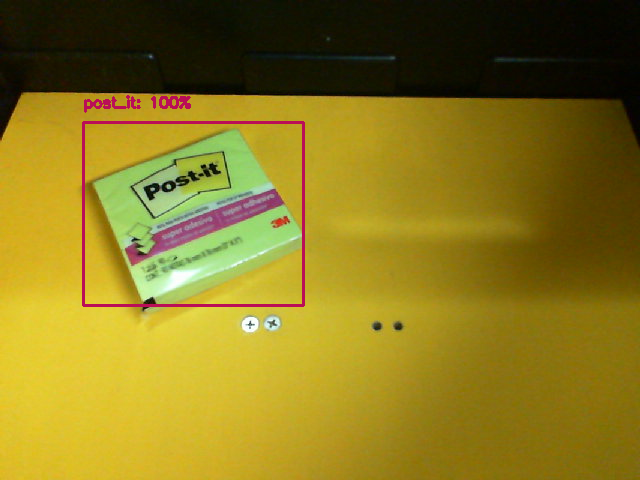
\includegraphics[width=.95\textwidth]{./images/singlelabel-classification-1.png}
%         \caption{}
%     \end{subfigure}
%     \begin{subfigure}{0.5\textwidth}
%         \centering
%         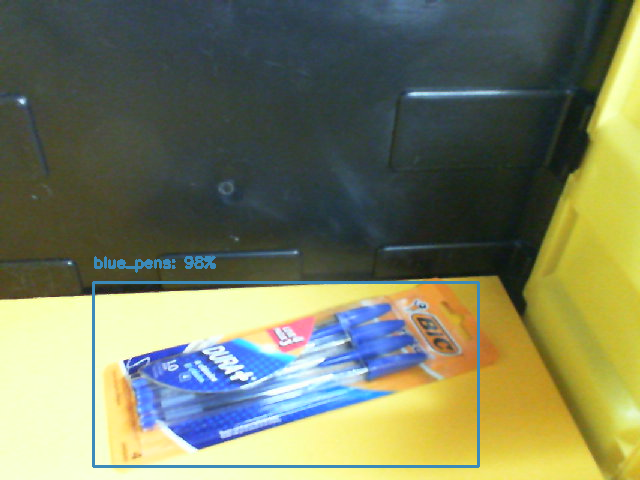
\includegraphics[width=.95\textwidth]{./images/singlelabel-classification-2.png}
%         \caption{}
%     \end{subfigure}
% 	\fonte{}
%     \label{fig:singleclassification}
% \end{figure}
% \begin{figure}[H]
%     \begin{subfigure}{0.5\textwidth}
%         \centering
%         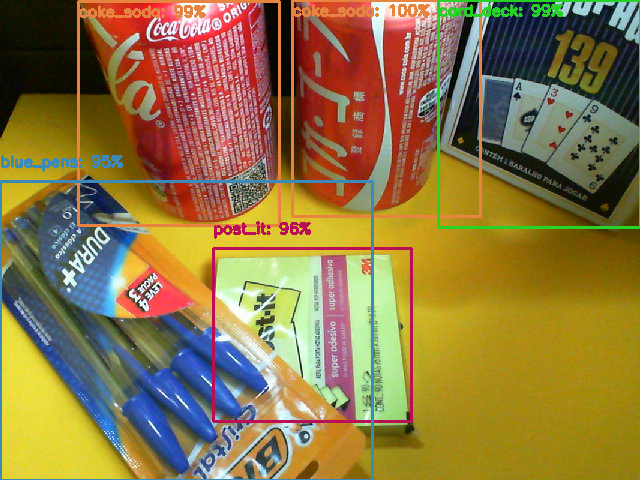
\includegraphics[width=.95\textwidth]{./images/multilabel-classification-1.png}
%         \caption{}
%     \end{subfigure}
%     \begin{subfigure}{0.5\textwidth}
%         \centering
%         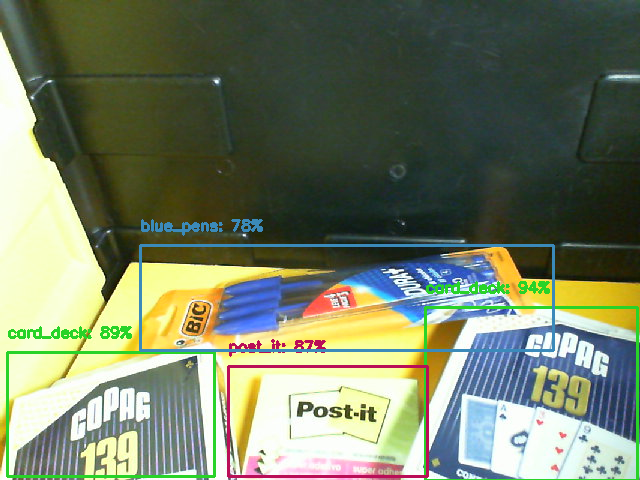
\includegraphics[width=.95\textwidth]{./images/multilabel-classification-2.png}
%         \caption{}
%     \end{subfigure}
% 	\caption[Multi-Label Classification Examples]{Multi-Label Classification Examples}
% 	\fonte{}
%     \label{fig:multiclassification}
% \end{figure}

The accuracy metrics were also inferred in our Test data set by using the TensorFlow Lite's 
Object Detector \textit{evaluate} method\footnote{https://www.tensorflow.org/lite/api\_docs/python/tflite\_model\_maker/object\_detector/ObjectDetector\#evaluate}
for all different model configurations that were applied. 
The main evaluation metrics for the models considered for our product, which were the ones based 
in the EfficientDet-D0, D1 and D2 architectures -- as the D3 and D4 architectures were too 
computationally expensive for our device -- are listed in Table 4. 

The numbers exhibited in the table consist of the classification Average Precision 
(\sigla{AP}{Average Precision}), which measures the percentage of correctly labeled 
predictions amongst all predictions; the AP with an IoU of 50\%, which means that
there is at least 50\% of overlap between the predicted and the actual bounding boxes; 
the AP with an IoU of 75\%; and the individual classification APs for each label that 
was forecasted. 

% \begin{table}[H]
% 	\label{tab:modelPerformance}
% 	\centering
% 	\caption[Test Evaluation Metrics for the Different Strategies and Models Applied for Inference]{Test Evaluation Metrics for the Different Strategies and Models Applied for Inference}
% 	\begin{adjustbox}{width=1\textwidth}
% 	\begin{tabular}{c|c|c|c|c|c|c|c|c|c|c}
% 		\hline 
% 		Architecture & Preprocessing Strategy & Training Strategy & AP & AP 50 IoU & AP 75 IoU & AP (post\_it) & AP (guarana) & AP (coke) & AP (card\_deck) & AP (blue\_pens) \\
% 		\hline
%         Efficientdet\-D0 & Resizing & Transfer Learning & \texttt{0.527} & \texttt{0.700} & \texttt{0.644} & \texttt{0.521} & \texttt{0.443} & \texttt{0.685} & \texttt{0.490} & \texttt{0.497} \\
% 		Efficientdet\-D1 & Resizing & Transfer Learning & \texttt{0.623} & \texttt{0.786} & \texttt{0.740} & \texttt{0.409} & \texttt{0.639} & \texttt{0.812} & \texttt{0.670} & \texttt{0.588} \\
% 		Efficientdet\-D2 & Resizing & Transfer Learning & \texttt{0.653} & \texttt{0.799} & \texttt{0.774} & \texttt{0.587} & \texttt{0.659} & \texttt{0.825} & \texttt{0.669} & \texttt{0.524} \\
% 		Efficientdet\-D0 & Resizing & Whole & \texttt{0.813} & \texttt{0.978} & \texttt{0.906} & \texttt{0.752} & \texttt{0.765} & \texttt{0.891} & \texttt{0.921} & \texttt{0.736} \\
% 		Efficientdet\-D1 & Resizing & Whole & \texttt{0.802} & \texttt{0.939} & \texttt{0.875} & \texttt{0.719} & \texttt{0.675} & \texttt{0.903} & \texttt{0.928} & \texttt{0.785} \\
% 		\textbf{Efficientdet\-D2} & \textbf{Resizing} & \textbf{Whole} & \textbf{0.826} & \textbf{0.967} & \textbf{0.922} & \textbf{0.763} & \textbf{0.776} & \textbf{0.910} & \textbf{0.895} & \textbf{0.784} \\
% 		Efficientdet\-D0 & Cropping & Transfer Learning & \texttt{0.490} & \texttt{0.668} & \texttt{0.592} & \texttt{0.357} & \texttt{0.422} & \texttt{0.595} & \texttt{0.633} & \texttt{0.443} \\
% 		Efficientdet\-D1 & Cropping & Transfer Learning & \texttt{0.580} & \texttt{0.730} & \texttt{0.686} & \texttt{0.312} & \texttt{0.605} & \texttt{0.716} & \texttt{0.736} & \texttt{0.531} \\
% 		Efficientdet\-D2 & Cropping & Transfer Learning & \texttt{0.562} & \texttt{0.722} & \texttt{0.699} & \texttt{0.463} & \texttt{0.569} & \texttt{0.576} & \texttt{0.661} & \texttt{0.539} \\
% 		Efficientdet\-D0 & Cropping & Whole & \texttt{0.832} & \texttt{0.954} & \texttt{0.934} & \texttt{0.869} & \texttt{0.854} & \texttt{0.717} & \texttt{0.922} & \texttt{0.800} \\
% 		Efficientdet\-D1 & Cropping & Whole & \texttt{0.792} & \texttt{0.897} & \texttt{0.880} & \texttt{0.823} & \texttt{0.763} & \texttt{0.586} & \texttt{0.933} & \texttt{0.852} \\
% 		Efficientdet\-D2 & Cropping & Whole & \texttt{0.803} & \texttt{0.923} & \texttt{0.893} & \texttt{0.795} & \texttt{0.808} & \texttt{0.631} & \texttt{0.941} & \texttt{0.840} \\
% 		\hline 
% 	\end{tabular}
% 	\end{adjustbox}
% 	\label{tab:modelPerformance}
% 	\fonte{}
% \end{table}

We could clearly see that, while the Transfer Learning models were much faster to train,
in our particular case, the Whole-trained models outperformed them. This could be 
due to the fact that our pictures and objects are different from the
ones that are present in the COCO-2017 dataset; or because a custom feature extractor- 
with custom hidden layer weights and biases- could have better performance with our pictures. 
In terms of the architectures, as expected, the D2 architecture offered more robust results, specially
amongst the models that applied resizing as a preprocessing strategy. 

We could not see much superior metrics for the models that used cropping for the images preprocessing, 
and that might be because most of the bounding boxes ended up being cropped as well and, with that, we lost
a portion of valuable label data. Altough the EfficientDet-D0 model that was Whole-Trained with Cropped images
had a comparable performance in our Test Data evaluation, considering the end-to-end usability tests that we executed 
with the assembled prototype and the overall better performance presented by the D2 architecture, as shown in
figure \ref{fig:yoloefficientdet}, we selected the EfficientDet-D2 model that was Whole-Trained with Resized
images as our champion model.

The loss (error) metrics during training were also computed for our Train and Validation sets during the 
200 epochs that were used for training our models using batches of 16 images, for all different 
settings that were employed to train them. We can clearly state that the model showed significant
improvement as the epochs progressed, and maybe more epochs would even have brought greater performance,
as the weights would have been even more fine-tuned. The trade-off, though, is that it would have 
taken more time and computer power to train the models.
In Figure \ref{fig:training}, you can find the Classification Loss chart for our three top models of choice, which were
the EfficientDet-D0, D1 and D2, whole-trained and that used resizing as a preprocessing strategy.

% \begin{figure}[H]
% 	\centering
%     \begin{subfigure}{0.65\textwidth}
%         \centering
%         \includegraphics[width=1\textwidth]{./images/efficientdet-d0-resized-whole-loss.png}
%         \caption{}
%     \end{subfigure}
%     \begin{subfigure}{0.65\textwidth}
%         \centering
%         \includegraphics[width=1\textwidth]{./images/efficientdet-d1-resized-whole-loss.png}
%         \caption{}
%     \end{subfigure}
%     \begin{subfigure}{0.65\textwidth}
%         \centering
%         \includegraphics[width=1\textwidth]{./images/efficientdet-d2-resized-whole-loss.png}
%         \caption{}
%     \end{subfigure}
% 	\caption[Train and Validation Classification Loss for the EfficientDet Models that 
% 		was whole-trained and took resized images as an input]{Train and Validation Classification Loss 
% 		for the EfficientDet Models that was whole-trained and took resized images as an input}
% 	\fonte{}
%     \label{fig:training}
% \end{figure}

Note that those spikes in the loss values are probably due to the batch size, as it could be 
that in specific batches of 16 images the model was not fully prepared to predict the labels
in those images. Using a larger batch would likely solve it, however it would also take more RAM
memory consumption. 

Finally, to improve inference time performance, we also compiled our TensorFlow Lite models for 
usage with an Edge TPU, which further reduced our inference times. 

\begin{table}[H]
	\centering
	\caption[Inference Performance Metrics with and without the TPU]{Inference Performance Metrics with and without the TPU}
	\begin{adjustbox}{width=1\textwidth}
	\label{tab:modelPerformance}
	\begin{tabular}{c|c|c|c|c}
		\hline 
		Model & FPS without the TPU & FPS using the TPU & CPU Ops using the TPU & TPU Ops using the TPU\\
		\hline
        Efficientdet-D0 Whole-Trained on Resized Images & \texttt{3.69} & \texttt{6.87} & \texttt{3} & \texttt{264}\\
		Efficientdet-D1 Whole-Trained on Resized Images & \texttt{2.09} & \texttt{5.14} & \texttt{131} & \texttt{191}\\
		Efficientdet-D2 Whole-Trained on Resized Images & \texttt{1.36} & \texttt{3.50} & \texttt{131} & \texttt{226}\\ 
		\hline 
	\end{tabular}
	\end{adjustbox}
	\fonte{Own work}
\end{table}

Figure \ref{fig:framecount} displays an example frame from the camera feed displaying the 
current FPS count.

\begin{figure}[H]
	\centering
    \caption[Frame from camera feed with FPS count]{Frame from camera feed with FPS count}
	\includegraphics[width=0.5\textwidth]{./images/frameratemeasurement.png}
    \label{fig:framecount}
    \fonte{}
\end{figure}

The inference speed has thoroughly improved - about 50\% on average - resulting
in a greater capability to process more Frames Per Second. When we look at the
number of CPU and TPU Operations, though, what we would expect when using the
TPU is that most Operations happen on the TPU side, however this behavior could
only be seen in the EfficientDet-D0 model. Part of it is because the
EfficientDet-D0 model has a simpler architecture, but it could also be due to
the conversion of the model for usage with the TPU or to the limited capacity
of the TPU device that was used. For instance, Google suggests using two TPU
cores for the EfficientDet-D2
model\footnote{https://www.tensorflow.org/lite/models/modify/model\_maker/object\_detection},
because the tensors are too large to fit in the chip's memory.

Overall, after considering the tradeoff between precision and performance, we
have decided to use the EfficientDet-D2 model since its performance when paired
with the Coral TPU was more than enough for our purposes (around 4 FPS) and had
the best precision, improving the overall experience of the prototype.

\section{Power Consumption}

For estimating the overall power consumption, a commercial wattmeter was used
to observe the total power required by the power adapter used, as shown in
Figure \ref{fig:wattmeter}.

\begin{figure}[H]
	\centering
	\caption[Power consumption measurement using a wattmeter]{Power consumption measurement using a wattmeter}
    \includegraphics[width=0.5\textwidth]{./images/powerconsumption.jpeg}
	\fonte{}
    \label{fig:wattmeter}
\end{figure}

During our tests, we have observed an average consumption of \textbf{10,4W}
when running the all the software and hardware components of the prototype
through an external power adapter. 

The tests were performed on a 220V power line using the following equipment:
\begin{itemize}
    \item Sinotimer DDS108 Digital Wattmeter
    \item Baseus Quick Charger GaN 65W
\end{itemize}

Since both of these products do not have detailed accuracy and efficiency data
available, we estimate an overall 10\% margin of error considering their
construction \cite{Chen2017}. 

With that, we can assume that the actual power draw is between 9,4W and 11,4W.
Considering a desired  battery life of 24 hours, it would require a battery of
about 240 Wh, which can be found commercially and would not impose a
insurmountable practical barrier.

\section{Cost}

One of the important aspects when developing a marketable product is its \textbf{cost}.

A more detailed overview of the items and their costs is shown on Table \ref{tbl:cost}.

\begin{table}[H]
	\centering
	\label{tab:correlacao}
    \caption[Items used on the prototype and their approximate retail cost in Brazil as of October 2022]{Items used on the prototype and their retail cost in October 2022}
	\begin{tabular}{c c c}
		\hline 
        Item & Quantity & Cost per item (BRL/USD) \\
		\hline
        Raspberry Pi 4 8GB Board &  1 & R\$ 1072,40 / US\$ 201,94 \\
        Coral Edge TPU &  1 & R\$ 318,51 / US\$ 59,99 \\
        HX711 with breakout board &  1  & R\$ 2,55 / US\$ 0,48 \\
        10Kg Load Cell & 1 & R\$ 6,89 / US\$ 1,30 \\
        MDF Board &  2  & R\$ 10,00 / US\$ 1,89 \\
        Mounting hardware (screws, bolts and nuts) &  1  & R\$ 5,00 / US\$ 0,94 \\
        Foldable utility cart &  1  & R\$ 125,00 / US\$ 23,60 \\
        Webcam &  1  & R\$ 100,00 / US\$ 18,88 \\
		\hline 
        & Total cost & R\$ 1650,35 / US\$ 310,91 \\
        \hline
	\end{tabular}
	\fonte{}
    \label{tbl:cost}
\end{table}

Of course, the developed prototype does not include all the necessary hardware
and software structure to deliver a successful product, but still it might show that at a
fundamental level, the cost of such a solution might not reach the costs that
current smart carts in the market sell for\footnote{The Nextop cart shown on the
introduction currently retails for R\$ 120.000}.

Therefore, it might be possible to conclude that most of the retail cost of the
existing smart carts is not composed of the production and infrastructure costs
but from the required repayment of the research and development costs that such
a product demand.

\section{Challenges and future work}

As one of the expected outcomes of our work, we have been able to identify
several practical challenges that would need to be worked on for a marketable
product and will be discussed in the next sections.

\subsection{Extending the model for new products}
In a supermarket use case, we expect that products will need to be added or
removed from detection model on a regular basis. That becomes a challenge when
we consider the amount of data necessary to train the model used in the
developed prototype.

Considering that, an important next step on the development would be to work on
a model that can be easily extend to support new products without requiring too
much computational power for retraining.

\subsection{Deploying updates}

Considering the compute locality of the detection model used in the prototype,
which is the board embedded in the cart, deploying updates to the model to it
might become a challenge.

Changing the compute locality to  a Cloud infrastructure \cite{Aws2022} might
allow for easier deployment for updates but that comes with a trade off in
terms of latency, since networks calls would be required, and that can become
detrimental in such a real-time based product.

Investigating that trade off or even developing a solution for easy deployment
of model updates is another import development to be worked in the future. 

\subsection{Batteries and charging}

Another challenge identified for creating a viable product is to develop and
energy efficient solution that is capable of running on a reasonable battery
for at least an entire day.

As described in the testing section, the prototype is already capable of being
deployed with a reasonable commercial battery but we believe that there are
still margin for improvement.

Evidently, it is possible to include a battery with bigger capacity to the
product to provide better battery life but that comes with the trade off of
additional weight and cost, undesired characteristics from the end user and
grosser perspective respectively.

Additionally, it would be important to developed a practical mechanism to allow
the carts to be charged such as a docking mechanism or even by wireless
charging \cite{Treffers2015}, reducing the maintenance effort from the grocery's
perspective. 

\subsection{Loss Prevention}

As our research has shown, loss prevention is a key feature of a smart cart, specially in the Brazilian context
\cite{Nextop2022}.

In such scenario, it would be important to work on possible extra features that
would give the grosser the extra confidence to deploy the cart to his/her retail
chain.

\subsection{Improving accuracy and reliability}

Related to the subsection above, improving the accuracy and reliability of the
overall system is key not just for loss prevention but to provide a great user
experience. We believe that a sub par experience will eventually lead to disuse
and therefore our objective would be to achieve a \textit{transparent}
experience, where the user might even forget about all the technological feat
that allows the cart to function.
%% Comente para remover este item

%% Capítulo - esse capítulo contém exemplos para melhor uso do modelo Latex
%% Na versão final do TCC esse capítulo deve ser removido utilizando o sinal %
%%%%% CAPÍTULO - EXEMPLO
%%
%% Capítulo de informações e exemplos de utilização deste modelo.

%% Título e rótulo de capítulo (rótulos não devem conter caracteres especiais, acentuados ou cedilha)
\chapter{Informações e Exemplos de Utilização deste Modelo}\label{cap:exemplo}

Devido à necessidade de padronização em trabalhos acadêmicos (teses, dissertações, trabalhos de conclusão de curso, etc.), são utilizadas neste documento algumas regras básicas para estruturação e formatação.

O presente documento/\textit{template} foi produzido em parceria entre a \gls{utfpr} de Pato Branco e a \gls{utfpr} de Campo Mourão. Assim, derivado do \gls{utfprpbtex}\index{UTFPRPBTeX@\utfprpbtex} e de alterações implementadas pela UTFPR de Campo Mourão, surge o \utfprtex, como um proposta de um modelo \latex que pode ser utilizado por qualquer campus da \gls{utfpr} para elaboração de trabalhos acadêmicos segundo as normas definidas pela \gls{abnt}\index{ABNT}. Este modelo foi desenvolvido em linguagem de editoração \gls{tex}\index{TeX@\TeX}/\gls{latex}\index{LaTeX@\latex} com base no modelo \gls{abntex2}\index{abnTeX2@\abnTeX} \cite{abnTeX2:2013}, que atende os requisitos das normas da ABNT para elaboração de documentos técnicos e científicos brasileiros.

Os principais arquivos do modelo são: 
\begin{itemize}
    \item \texttt{main.tex} - é o arquivo principal que relaciona todos os outros arquivos, neste você pode remover ou adicionar elementos textuais (capítulos, etc);
    \item \texttt{configuracoes.tex} - contém os pacotes a serem utilizados pelo ambiente, bem como a criação de comandos do \latex;
    \item \texttt{variaveis.tex} - contém variáveis, como nome do autor, orientador, título, banca e que devem ser alterados para atender cada trabalho;
    \item \texttt{main.bib} - contém as referências bibliográficas;
    \item \texttt{readme.md} - são informações a respeito do template \latex;
    \item \texttt{utfpr.cls} - mantém a formatação do texto - \textbf{não altere esse arquivo a menos que você saiba o que está fazendo}.
\end{itemize}

Além dos arquivos, o \textit{template} contém diretórios/pastas, para ajudar a organizar o trabalho, sendo essas:
\begin{itemize}%% Lista de itens
\item \texttt{PreTexto} - contém arquivos, com nomes auto descritivos, que representam elementos pré textuais como:  resumo, abstract, agradecimentos, siglas, epigrafe, etc;
\item \texttt{capitulos} -  contém arquivos, com nomes auto descritivos, que representam os capítulos do texto, como por exemplo: introdução, metodologia, conclusão, etc. Para adicionar ou remover um capítulo é necessário alterar o arquivo \texttt{main.tex} - ver exemplos no próprio arquivo;
\item \texttt{figuras}  - contém as figuras/imagens utilizadas no texto;
\item \texttt{PosTexto} - contém elementos pós textuais como: anexo, apêndice, etc.
\end{itemize}

A codificação de caracteres em todos os arquivos é \texttt{UTF8}, tanto no modelo \gls{abntex2}\index{abnTeX2@\abnTeX} quanto no modelo \gls{utfprpbtex}\index{UTFPRPBTeX@\utfprtex}. Portanto, é necessário que seja utilizada a mesma codificação nos documentos a serem desenvolvidos, inclusive nos arquivos de base bibliográfica. Diversos editores de arquivos fonte do \gls{latex}\index{LaTeX@\latex} são capazes de manipular e/ou converter entre diferentes codificações, por exemplo, o ``Texmaker\index{Texmaker}'' (disponível em \url{http://www.xm1math.net/texmaker/}). 
%Recomenda-se, sempre que for manipular e/ou substituir um dos arquivos constituintes deste modelo, manter uma cópia do original num local seguro e/ou renomear esta cópia do original para que possa ser utilizada como um exemplo no desenvolvimento do seu próprio arquivo. Por exemplo, quando for criar o seu ``Capítulo 1'', fazer uma cópia do arquivo original \texttt{capitulo1.tex}, renomeando-o para \texttt{capitulo1.original.tex}, por exemplo, e realizar as alterações e/ou modificações no arquivo \texttt{capitulo1.tex}.

Este capítulo\label{errata:capitulo} de exemplo tem por finalidade a definição e a apresentação de alguns comandos do \gls{latex}\index{LaTeX@\latex} e/ou dos modelos \gls{abntex2}\index{abnTeX2@\abnTeX} e \gls{utfprpbtex}\index{UTFPRPBTeX@\utfprtex}. O presente documento não se constitui um manual, tampouco uma apostila de \gls{latex}\index{LaTeX@\latex}, visto que existe uma grande quantidade de material de referência disponível na Internet, como por exemplo em \url{http://en.wikibooks.org/wiki/LaTeX}.

Os capítulos devem conter uma introdução e um fecho. A introdução fornece ao leitor uma breve descrição do que será tratado no capítulo, enquanto o fecho apresenta comentários finais sobre o que foi desenvolvido no capítulo. Os capítulos podem ser divididos em seções\label{errata:secao}. Esta divisão deve ser lógica (temática) e não física (por tamanho). O número ideal de seções é impossível de se precisar. Entretanto, um capítulo com uma única seção, possivelmente, deverá ser agregado ao capítulo anterior ou posterior. Um capítulo com quinze seções, possivelmente, deverá ser subdividido em dois capítulos. Capítulos, seções e subseções\label{errata:subsecao} devem ser rotulados para que possam ser referenciados em qualquer parte do texto. Exemplo: O \autoref{cap:exemplo} é gerado, rotulado e referenciado pelos comandos \verb|\chapter{Informações e...}|, \verb|\label{cap:exemplo}| e \verb|\autoref{cap:exemplo}|, respectivamente.

%% Título e rótulo de seção (rótulos não devem conter caracteres especiais, acentuados ou cedilha)
\section{Título da seção secundária}\label{sec:secsec}

Seções secundárias são divisões do conteúdo das seções primárias. A \autoref{sec:secsec} é gerada, rotulada e referenciada pelos comandos \verb|\section{Título da Seção Secundária}|, \verb|\label{sec:secsec}| e \verb|\autoref{sec:secsec}|, respectivamente.

%% Título e rótulo de seção (rótulos não devem conter caracteres especiais, acentuados ou cedilha)
\subsection{Título da seção terciária}\label{ssec:secterc}

Seções terciárias são divisões do conteúdo de seções secundárias. A \autoref{ssec:secterc} é gerada, rotulada e referenciada pelos comandos \verb|\subsection{Título da Seção Terciária}|, \verb|\label{ssec:secterc}| e \verb|\autoref{ssec:secterc}|, respectivamente.

%% Título e rótulo de seção (rótulos não devem conter caracteres especiais, acentuados ou cedilha)
\subsubsection{Título da seção quartenária}\label{sssec:secquart}

Seções quartenárias são divisões do conteúdo de seções terciárias. A \autoref{sssec:secquart} é gerada, rotulada e referenciada pelos comandos \verb|\subsubsection{Título da seção quartenária}|, \verb|\label{sssec:secquart}| e \verb|\autoref{sssec:secquart}|, respectivamente.

%% Título e rótulo de seção (rótulos não devem conter caracteres especiais, acentuados ou cedilha)
\section{Exemplo de título de seção secundária com um texto muito longo que pode ocupar mais de uma linha}\label{sec:sectitulolongo}

A \autoref{sec:sectitulolongo} é um exemplo de título de seção secundária com texto muito longo, formatado automaticamente de acordo com \citeonline[subseções 5.2.2 a 5.2.4]{NBR14724:2011} e \citeonline[subseções 3.1 a 3.8]{NBR6024:2012}. Segundo as normas, o título de seção deve estar alinhado à esquerda e a segunda e demais linhas devem iniciar logo abaixo da primeira palavra da primeira linha.

%% Título e rótulo de seção (rótulos não devem conter caracteres especiais, acentuados ou cedilha)
\section{Elementos pré-textuais}\label{sec:elempretext}

Alguns elementos pré-textuais do presente documento são gerados automaticamente pelo \gls{utfprpbtex}\index{UTFPRPBTeX@\utfprtex}. Para adicionar e/ou alterar as informações apresentadas na capa, na folha de rosto %, na ficha catalográfica 
e na folha de aprovação deve-se editar o arquivo \texttt{variaveis.tex}. %Os dados informados neste arquivo também são utilizados para gerar a referência do trabalho na errata, no resumo e no \textit{abstract}.

Para adicionar e/ou alterar o texto da errata, da dedicatória, dos agradecimentos, da epígrafe, do resumo e do \textit{abstract} deve-se editar seus respectivos arquivos presentes no diretório ``PreTexto'': \texttt{errata.tex}, \texttt{dedicatoria.tex}, \texttt{agradecimentos.tex}, \texttt{epigrafe.tex}, \texttt{resumo.tex} e \texttt{abstract.tex}.

As listas de algoritmos, de ilustrações e de tabelas são geradas automaticamente pelo \gls{utfprpbtex}\index{UTFPRPBTeX@\utfprtex}. Os itens destas listas são gerados a medida que forem sendo inseridos no texto do documento. 

A lista de abreviaturas, siglas e acrônimos pode ser gerada automaticamente por meio do arquivo \texttt{entradas-acronimos.tex}, utilizando o pacote \texttt{glossaries}\footnote{Detalhes sobre comandos para geração de abreviaturas, siglas e acrônimos utilizando o pacote \texttt{glossaries} são apresentadas na \autoref{sec:acronimos}.}, ou por meio da edição do arquivo \texttt{lista-acronimos.tex}. A lista de símbolos pode ser gerada automaticamente utilizando o pacote \texttt{nomencl}\footnote{Detalhes sobre comandos para geração de símbolos utilizando o pacote \texttt{nomencl} são apresentadas na \autoref{sec:simbolos}.} ou mediante a edição do arquivo \texttt{lista-simbolos.tex}. Os arquivos citados estão no diretório ``PreTexto''. O sumário é o último elemento pré-textual e também é gerado automaticamente pelo \gls{utfprpbtex}\index{UTFPRPBTeX@\utfprtex}.

%% Título e rótulo de seção (rótulos não devem conter caracteres especiais, acentuados ou cedilha)
\section{Regras gerais de apresentação}\label{sec:regrasgerais}

As regras gerais de apresentação, definidas na sequência, já estão predefinidas no modelo \gls{utfprpbtex}\index{UTFPRPBTeX@\utfprtex}. Algumas destas regras podem ser alteradas, por comandos apropriados do \gls{latex}\index{LaTeX@\latex}, do \gls{abntex2}\index{abnTeX2@\abnTeX} ou do \gls{utfprpbtex}\index{UTFPRPBTeX@\utfprtex}, no preâmbulo do arquivo principal \texttt{configuracoes.tex} ou em outras partes do documento, por exemplo, nos capítulos.

\begin{itemize}%% Lista de itens
\item Configuração das margens: deve-se usar margens superior e esquerda de \SI{3}{cm}; e margens inferior e direita de \SI{2}{cm}; em papel formato A4 ($\SI{21}{cm} \times \SI{29,7}{cm}$);
\item Recomenda-se o uso de fonte tipo Arial ou Times New Roman, tamanho 12 para o texto e tamanho 10 para citações de mais de três linhas, notas de rodapé e legendas dos algoritmos, ilustrações e tabelas;
\item O parágrafo deve aparecer com recuo na primeira linha de \SI{1,5}{cm}, justificado, sem espaçamento anterior ou posterior;
%\item Os elementos como: o resumo, as notas, as referências, as legendas das ilustrações e tabelas, a natureza do trabalho, o objetivo, o nome da instituição a que é submetida e a área de concentração devem ser digitados em espaço simples.
\item A numeração progressiva para as seções do texto deve ser adotada para evidenciar a sistematização do conteúdo do trabalho;
\item Para os títulos das seções não se utilizam pontos, hífen, travessão, ou qualquer sinal após o indicativo de seção ou de título;
\item Para as seções primárias: utiliza-se negrito e caixa alta;
\item Para as seções secundárias: título em negrito, iniciado em letra maiúscula e demais letras minúsculas;
\item Para as seções terciárias: somente a primeira letra do título da seção em
maiúscula;
\item Para as seções quaternárias: título da seção sublinhado, com inicial em letra maiúscula e demais letras minúsculas.
\item No sumário, os títulos das seções devem aparecer exatamente iguais ao que estão contidos no trabalho.
\end{itemize}

\caixa{Atenção}{No \latex é necessário manter os títulos apenas com a primeira letra maiúscula e o restante em minúsculo, o retante é controlado pelo \latex, então não é necessário se preocupar com a formatação!}

Recomenda-se evitar, sempre que possível, o uso dos seguintes recursos (ou enfeites) no documento:

\begin{itemize}%% Lista de itens
\item \textbf{o uso de negrito;}
\item \textit{o uso de itálico (exceto em palavras em outra língua);}
\item \texttt{texto em diferente fonte como máquina de escrever;}
\item \underline{o uso de texto sublinhado;}
\item o uso excessivo de\footnote{Notas de rodapé.}.
\end{itemize}

\noindent Lembre-se: um texto ``limpo'' é mais agradável de ler que um texto ``enfeitado''.

%% Título e rótulo de seção (rótulos não devem conter caracteres especiais, acentuados ou cedilha)
\subsection{Espaçamento}\label{sec:espacamento}

\begin{itemize}%% Lista de itens
%\item O resumo, o \textit{abstract}, as notas, as referências, as legendas das ilustrações e tabelas e a natureza do trabalho devem ser digitadas em espaço simples.
\item Todo o texto deve ser formatado com espaço entre linhas de um fator de 1,5 (sem espaçamento antes/depois).
\item As citações com mais de três linhas devem ser em espaço simples e com recuo de \SI{4}{cm} da margem esquerda.
\item As referências, ao final do trabalho, devem ser separadas entre si por um espaços simples, e na mesma referência o espaço é simples.
%\item Os títulos das seções secundárias devem ser separados do texto que os precede por dois espaços entre linhas de um fator de 1,5.
\item As seções primárias devem iniciar em páginas distintas.
\end{itemize}

O recuo na primeira linha, espaço entre a margem e o início do parágrafo, pode ser redefinido definido pelo comando:

\begin{SingleSpacing}%% Ambiente SingleSpacing
\begin{verbatim}
\setlength{\parindent}{1.5cm}
\end{verbatim}
\end{SingleSpacing}

O espaçamento entre um parágrafo e outro\index{espaçamento!entre os parágrafos} pode ser redefinido pelo comando:

\begin{SingleSpacing}%% Ambiente SingleSpacing
\begin{verbatim}
\setlength{\parskip}{0mm} %% Tente também \onelineskip
\end{verbatim}
\end{SingleSpacing}

O controle do espaçamento entre linhas\index{espaçamento!entre as linhas} pode ser redefinido pelo comando:

\begin{SingleSpacing}%% Ambiente SingleSpacing
\begin{verbatim}
\OnehalfSpacing %% Espaçamento um e meio (padrão)
\DoubleSpacing  %% Espaçamento duplo
\SingleSpacing  %% Espaçamento simples
\end{verbatim}
\end{SingleSpacing}

Para isso, também estão disponíveis os ambientes:

\begin{SingleSpacing}%% Ambiente SingleSpacing
\begin{verbatim}
\begin{SingleSpacing} ...     \end{SingleSpacing}
\begin{Spacing}{<factor>} ... \end{Spacing}
\begin{OnehalfSpacing} ...    \end{OnehalfSpacing}
\begin{OnehalfSpacing*} ...   \end{OnehalfSpacing*}
\begin{DoubleSpacing} ...     \end{DoubleSpacing}
\begin{DoubleSpacing*} ...    \end{DoubleSpacing*}
\end{verbatim}
\end{SingleSpacing}

Para mais informações, consulte \citeonline[p. 47-52 e 135]{Wilson2010}.

\subsection{Exemplo de quantidades de subseções}\label{sec:exSubsec}

Quando um item é dividido, precisa ter pelo menos dois sub-itens (não pode ter apenas um), por exemplo para ter a subseção 4.1 é obrigatório ter pelo menos a subseção 4.2, não pode somente a primeira subseção.

%% Título e rótulo de seção (rótulos não devem conter caracteres especiais, acentuados ou cedilha)
\section{Enumerações: alíneas e subalíneas}\label{sec:enumeracoes}\index{alíneas}\index{subalíneas}

Quando for necessário enumerar os diversos assuntos de uma seção que não possua título, esta deve ser subdividida em alíneas\index{alíneas} \cite[subseção 4.2]{NBR6024:2012}:

\begin{alineas}%% Ambiente alineas
\item os diversos assuntos que não possuam título próprio, dentro de uma mesma seção, devem ser subdivididos em alíneas\index{alíneas};
\item o texto que antecede as alíneas\index{alíneas} termina em dois pontos;
\item as alíneas\index{alíneas} devem ser indicadas alfabeticamente, em letra minúscula, seguida de parêntese. Utilizam-se letras dobradas, quando esgotadas as letras do alfabeto;
\item as letras indicativas das alíneas\index{alíneas} devem apresentar recuo em relação à margem esquerda;
\item o texto da alínea deve começar por letra minúscula e terminar em ponto-e-vírgula, exceto a última alínea que termina em ponto final;
\item o texto da alínea deve terminar em dois pontos, se houver subalínea;
\item a segunda e as seguintes linhas do texto da alínea começa sob a primeira letra do texto da própria alínea;
\item subalíneas\index{subalíneas} \cite[subseção 4.3]{NBR6024:2012} devem ser conforme as alíneas\index{alíneas} a seguir:
\begin{alineas}%% Ambiente alineas
\item as subalíneas\index{subalíneas} devem começar por travessão seguido de espaço;
\item as subalíneas\index{subalíneas} devem apresentar recuo em relação à alínea;
\item o texto da subalínea deve começar por letra minúscula e terminar em ponto-e-vírgula. A última subalínea deve terminar em ponto final, se não houver alínea subsequente;
\item a segunda e as seguintes linhas do texto da subalínea começam sob a primeira letra do texto da própria subalínea.
\end{alineas}
\item no \gls{abntex2}\index{abnTeX2@\abnTeX} estão disponíveis os ambientes \texttt{incisos} e \texttt{subalineas}, que em suma são o mesmo que se criar outro nível de \texttt{alineas}, como nos exemplos à seguir:
\begin{incisos}%% Ambiente incisos
\item \textit{um novo inciso em itálico}\index{incisos}.
\end{incisos}
\item Alínea em \textbf{negrito}:
\begin{subalineas}%% Ambiente subalineas
\item \textit{uma subalínea em itálico};
\item \underline{\textit{uma subalínea em itálico e sublinhado}}.
\end{subalineas}
\item última alínea com \emph{ênfase}.
\end{alineas}

%% Título e rótulo de seção (rótulos não devem conter caracteres especiais, acentuados ou cedilha)
\section{Citações}\label{sec:citacoes}

O \gls{utfprpbtex}\index{UTFPRPBTeX@\utfprtex} está configurado para produzir as citações no texto no estilo alfabético (autor-data), segundo as normas \gls{abnt}\index{ABNT}, por meio dos comandos do \gls{abntex2}\index{abnTeX2@\abnTeX} \cite{abnTeX2:2013Cite,abnTeX2:2013CiteAlf}. A lista dos principais comandos são apresentadas a seguir:

\begin{itemize}%% Lista de itens
\item \verb|\cite{rótulo}| -- para gerar citação implícita. Por exemplo, a citação ``\ldots\ \cite{Thompson2001}\ldots'' é gerada pelo comando \verb|\cite{Thompson2001}| ou pelo atalho \verb|\citep{Thompson2001}|, definido em \texttt{utfprpb.tex}.
\item \verb|\citeonline{rótulo}| -- para gerar citação explícita. Por exemplo a citação ``\ldots\ conforme proposto por \citeonline{Thompson2001}\ldots'' é gerada pelo comando \verb|\citeonline{Thompson2001}| ou pelo atalho \verb|\citet{Thompson2001}|, definido em \texttt{utfprpb.tex}.
\item \verb|(\citeauthor{rótulo})| -- para gerar citação implícita somente do autor. Por exemplo, a citação ``\ldots\ (\citeauthor{Thompson2001})\ldots'' é gerada pelo comando \verb|(\citeauthor{Thompson2001})| ou pelo atalho \verb|\citepa{Thompson2001}|, definido em \texttt{utfprpb.tex}.
\item \verb|\citeauthoronline{rótulo}| -- para gerar citação explícita somente do autor. Por exemplo, a citação ``\ldots\ conforme a relação de \citeauthoronline{Thompson2001}\ldots'' é gerada pelo comando \verb|\citeauthoronline{Thompson2001}| ou pelo atalho \verb|\citeta{Thompson2001}|, definido em \texttt{utfprpb.tex}.
\item \verb|(\citeyear{rótulo})| -- para gerar citação implícita somente do ano. Por exemplo, a citação ``\ldots\ (\citeyear{Thompson2001})\ldots'' é gerada pelo comando \verb|(\citeyear{Thompson2001})| ou pelo atalho \verb|\citepy{Thompson2001}|, definido em \texttt{utfprpb.tex}.
\item \verb|\citeyear{rótulo}| -- para gerar citação explícita somente do ano. Por exemplo, a citação ``\ldots\ no ano de \citeyear{Thompson2001}\ldots'' é gerada pelo comando \verb|\citeyear{Thompson2001}| ou pelo atalho \verb|\citety{Thompson2001}|, definido em \texttt{utfprpb.tex}.
\end{itemize}

Informações sobre a utilização dos comandos listados acima e os demais comandos para geração de referências, utilizados pelo \gls{abntex2}\index{abnTeX2@\abnTeX}, podem ser encontradas em \citeonline{abnTeX2:2013Cite,abnTeX2:2013CiteAlf}, disponíveis em \url{http://www.abntex.net.br/}.

\gls{latex}\index{LaTeX@\latex} utiliza um arquivo externo (em separado) para o banco de dados das referências citadas no texto. Este arquivo é compilado pelo \gls{bibtex}\index{BibTeX@Bib\TeX} e deve possuir a extensão \texttt{bib}, como nos arquivos \texttt{referencias.bib} e \texttt{referencias-modelos.bib} presentes no diretório ``PosTexto'', utilizados neste documento. O arquivo \texttt{referencias-modelos.bib} apresenta exemplos dos seguintes estilos de referência aceitos pelo \gls{bibtex}\index{BibTeX@Bib\TeX}:

\begin{itemize}%% Lista de itens
\item anais de simpósios \citep{Alt1995,Pirmez2002};
\item artigos em anais de simpósios \citep{Faina2001};
\item artigos em coletâneas de artigos \citep{Pinto2000};
\item artigos em revistas \citep{Guimaraes2003};
\item capítulos de livros \citep{Santos2000};
\item livretos \citep{Thompson2001};
\item livros \citep{Pedrycz1998};
\item manuais técnicos \citep{IONA1999};
\item miscelânea \citep{Cruz2003};
\item páginas na Internet \cite[acessado em 1 de janeiro de 2004]{Larsson2003} (utilizar a data do último acesso à página);
\item relatórios técnicos \citep{OMG2000};
\item teses de mestrado \citep{SantosFilho2003};
\item teses de doutorado \citep{Faina2000};
\item trabalhos não publicados \citep{Sichman2002}.
\end{itemize}

\subsection{Programas úteis para citações}\label{sec:progUteisCitacoes}

Existem alguns programas para gerenciamento de banco de dados de referências bibliográficas (arquivos \texttt{bib}) do \gls{bibtex}\index{BibTeX@Bib\TeX}. O ``JabRef'' é um exemplo destes programas e está disponível em: \url{http://jabref.sourceforge.net/}.

%% Título e rótulo de seção (rótulos não devem conter caracteres especiais, acentuados ou cedilha)
\subsection{Citações diretas}\label{sec:citacoesdiretas}\index{citações!diretas}

O ambiente \texttt{citacao} permite a inclusão de citações diretas que ocupam mais de três linhas:

\begin{citacao}%% Ambiente citacao
As citações diretas no texto, que ocupam mais de três linhas, devem ser destacadas com recuo de \SI{4}{cm} da margem esquerda, com letra menor que a do texto utilizado e sem as aspas. No caso de documentos datilografados, deve-se observar apenas o recuo \cite[subseção 5.3]{NBR10520:2002}.
\end{citacao}

\noindent Esta citação direta com mais de três linhas foi gerada da seguinte forma:

\begin{SingleSpacing}%% Ambiente SingleSpacing
\begin{verbatim}
\begin{citacao}
As citações diretas no texto, com mais de três linhas,...
... observar apenas o recuo \cite[subseção 5.3]{NBR10520:2002}.
\end{citacao}
\end{verbatim}
\end{SingleSpacing}

O ambiente \texttt{citacao} pode receber como parâmetro opcional um nome de idioma previamente carregado nas opções da classe (definido no preâmbulo do arquivo \texttt{utfprpb.tex}). Neste caso, o texto da citação é automaticamente escrito em itálico e a hifenização é ajustada para o idioma selecionado na opção do ambiente. Por exemplo:

\begin{SingleSpacing}%% Ambiente SingleSpacing
\begin{verbatim}
\begin{citacao}[english]
Text in English language in italic with correct hyphenation.
\end{citacao}
\end{verbatim}
\end{SingleSpacing}

\noindent Tem como resultado:

\begin{citacao}[english]%% Ambiente citacao
Text in English language in italic with correct hyphenation.
\end{citacao}

Citações simples\index{citações!simples}, com até três linhas, devem ser incluídas com aspas. Observe que em \gls{latex}\index{LaTeX@\latex} as aspas iniciais são diferentes das finais: ``Amor é fogo que arde sem se ver''.

%% Título e rótulo de seção (rótulos não devem conter caracteres especiais, acentuados ou cedilha)
\section{Equações}\label{sec:equacoes}

\gls{latex}\index{LaTeX@\latex} é insuperável no processamento de equações. Equações simples como $y = a x^2 + b x + c$ podem ser adicionadas ao longo do texto ou em uma linha própria:
%
\[%% Ambiente displaymath
y = a x^2 + b x + c
\]

Equações complexas como:
%
\begin{equation}%% Ambiente equation
\label{eq:equation1}%% Rótulo
\begin{array}{lcl}%% Ambiente array
p \left(\gamma\right)
& = &
\frac{1}{2}
\sqrt{\frac{M}{\gamma \bar{\gamma}_b}}
\frac{1}{\prod_{i = 1}^M \sqrt{\tilde{\gamma}_i}}
\int_0^{\sqrt{M \delta}}
\int_0^{\sqrt{M \delta} - r_M} \cdots
\int_0^{\sqrt{M \delta} - \sum_{i = 3}^M r_i} \\[0.5\linha]
& &
p \left(%
\frac{\sqrt{M \delta} - \sum_{i = 2}^M r_i}{\sqrt{\tilde{\gamma}_1}},
\frac{r_2}{\sqrt{\tilde{\gamma}_2}}, \ldots,
\frac{r_M}{\sqrt{\tilde{\gamma}_M}}
\right) \, \der r_2 \cdots \der r_{M - 1} \, \der r_M
\end{array}
\end{equation}

\noindent ou
%
\begin{equation}%% Ambiente equation
\label{eq:equation2}%% Rótulo
T \left(r\right) =
\frac{1}{f_m}
\left(%
\frac{\pi}{2} \sum_{i = 1}^M {\tilde{r}_i^2 \dot{\varsigma}_i^2}
\right)^{-1/2}
\frac{%
\begin{array}{ll}%% Ambiente array
\int_0^{\rho \sqrt{M}}
\int_0^{\rho \sqrt{M} - r_M} \cdots
\int_0^{\rho \sqrt{M} - \sum_{i = 3}^M r_i}
\int_0^{\rho \sqrt{M} - \sum_{i = 2}^M r_i} \\[0.5\linha]
p \left(%
\frac{r_1}{\tilde{r}_1},
\frac{r_2}{\tilde{r}_2}, \ldots,
\frac{r_M}{\tilde{r}_M}
\right) \, \der r_1 \, \der r_2 \cdots \der r_{M - 1} \, \der r_M \\[0.5\linha]
\end{array}
}{%
\begin{array}{ll}%% Ambiente array
\int_0^{\rho \sqrt{M}}
\int_0^{\rho \sqrt{M} - r_M} \cdots
\int_0^{\rho \sqrt{M} - \sum_{i = 3}^M r_i} \\[0.5\linha]
p \left(%
\frac{\rho \sqrt{M} - \sum_{i = 2}^M r_i}{\tilde{r}_1},
\frac{r_2}{\tilde{r}_2}, \ldots,
\frac{r_M}{\tilde{r}_M}
\right) \, \der r_2 \cdots \der r_{M - 1} \, \der r_M \\[0.5\linha]
\end{array}
}
\end{equation}

\noindent são automaticamente numeradas e podem ser referenciadas ao longo do texto. Por exemplo, a \seqref{eq:equation1} é trivialmente derivada da \seqref{eq:equation2}. Veja os exemplos de comandos para estas equações no arquivo fonte deste capítulo.

%% Título e rótulo de seção (rótulos não devem conter caracteres especiais, acentuados ou cedilha)
\section{Algoritmos}\label{sec:algoritmos}

Algoritmos podem ser inseridos por meio do pacote \texttt{algorithms}, conforme exemplos no arquivo fonte deste capítulo e cujos resultados são apresentados no \autoref{alg:algoritmo1} e no \autoref{alg:algoritmo2}.

\begin{algorithm}[htb]%% Ambiente algorithm
\caption{Primeiro exemplo de algoritmo com uma legenda contendo um texto muito longo que pode ocupar mais de uma linha}%% Legenda
\label{alg:algoritmo1}%% Rótulo
\hrule
\begin{algorithmic}[1]%% Ambiente algorithmic
\ENSURE $A, B$
\STATE $C = A + B$
\PRINT $C$
\end{algorithmic}
\hrule
\fonte{}%% Fonte
\end{algorithm}

\begin{algorithm}[htb]%% Ambiente algorithm
\caption{Segundo exemplo de algoritmo}%% Legenda
\label{alg:algoritmo2}%% Rótulo
\hrule
\begin{algorithmic}[1]%% Ambiente algorithmic
\ENSURE $A, B$
\STATE $C = A + B$
\IF{$C < 10$}
\STATE $C = 2 \ C$
\ELSE
\STATE $C = 0,5 \ C$
\ENDIF
\PRINT $A, B, C$
\end{algorithmic}
\hrule
\fonte{}%% Fonte
\end{algorithm}

A documentação sobre o pacote \texttt{algorithms} pode ser encontrada em: \url{http://tug.ctan.org/tex-archive/macros/latex/contrib/algorithms/algorithms.pdf}.

%% Título e rótulo de seção (rótulos não devem conter caracteres especiais, acentuados ou cedilha)
\section{Ilustrações}\label{sec:ilustracoes}

O \gls{utfprpbtex}\index{UTFPRPBTeX@\utfprtex} está configurado para produzir os ambientes para os seguintes tipos de ilustrações: figuras, fotografias, gráficos e quadros. Exemplos de uso destes ambientes podem ser observados no arquivo fonte deste capítulo.

%% Título e rótulo de seção (rótulos não devem conter caracteres especiais, acentuados ou cedilha)
\subsection{Figuras}\label{sec:figuras}

Figuras são criadas e/ou editadas com editores gráficos capazes de exportar a figura em formato \gls{ps} ou, preferencialmente, \gls{eps}. O editor ``xfig'' é adequado para a maioria dos casos, como por exemplo, a \autoref{fig:figura1} que foi editada utilizando o ``xfig''. Outras opções para criação/edição de figuras são o GIMP (\url{http://www.gimp.org/}), ou o ``dia'' (\url{http://dia-installer.de/}), um editor orientado a diagramas (UML, fluxograma, etc.) com capacidade de exportar \gls{eps}, como apresentado por \citet{Larsson2003}.

%\gls{gimp}\index{Gimp}
\begin{figure}[htb]%% Ambiente figure
%\captionsetup{width=0.55\textwidth}%% Largura da legenda
\caption{Exemplo de figura criada a partir de um arquivo}%% Legenda
\label{fig:figura1}%% Rótulo
\includegraphics[width=0.6\textwidth]{figura1}%% Dimensões e localização
\fonte{\citet{Larsson2003}}%% Fonte
\end{figure}

Figuras em formato GIF, JPEG e BMP podem ser convertidas para o formato \gls{eps} por meio do aplicativo ``xv''. O ``xv'' não lista o formato \gls{eps} dentre aqueles que é capaz de manipular. Entretanto, selecionando-se o formato \textit{PostScript} e fornecendo-se a extensão \texttt{eps} ao nome do arquivo, o formato \gls{eps} é gerado.

O ambiente \texttt{picture} permite a programação de imagens diretamente no \gls{latex}\index{LaTeX@\latex}, conforme exemplo apresentado na \autoref{fig:figura2}.

\begin{figure}[htb]%% Ambiente figure
%\captionsetup{width=8cm}%% Largura da legenda
\caption{Exemplo de figura criada a partir do ambiente \texttt{picture}}%% Legenda
\label{fig:figura2}%% Rótulo
\setlength{\unitlength}{1cm}%% Unidade de comprimento
\begin{picture}(8,5)(-4,-2.5)%% Ambiente picture
\put(-4,0){\vector(1,0){8}}
\put(3.75,-0.25){$\chi$}
\put(0,-2.5){\vector(0,1){5}}
\multiput(-4,1)(0.4,0){20}{\line(1,0){0.2}}
\multiput(-4,-1)(0.4,0){20}{\line(1,0){0.2}}
\put(0.25,2.25){$\beta \equiv v / c = \tanh \chi$}
\qbezier(0,0)(0.8853,0.8853)(2,0.9640)
\qbezier(0,0)(-0.8853,-0.8853)(-2,-0.9640)
\end{picture}
\fonte{}%% Fonte
\end{figure}

%% Título e rótulo de seção (rótulos não devem conter caracteres especiais, acentuados ou cedilha)
\subsection{Fotografias}\label{sec:fotografias}

Um exemplo deste tipo de ilustração é apresentado na \autoref{foto:foto1}.

\begin{photograph}[htb]%% Ambiente photograph
%\captionsetup{width=0.6\textwidth}%% Largura da legenda
\caption{Camaleão pantera fotografado por Joel Sartore, National Geographic}%% Legenda
\label{foto:foto1}%% Rótulo
\includegraphics[width=0.95\textwidth]{foto1}%% Dimensões e localização
\fonte{\citet{Sartore2013}}%% Fonte
\end{photograph}

Outro exemplo deste tipo de ilustração é apresentado na \autoref{foto:foto2}.

\begin{photograph}[htb]%% Ambiente photograph
\captionsetup{width=0.6\textwidth}%% Largura da legenda
\caption{Fotografia da erupção vulcânica em 1982 do Galungung, Indonésia (com descargas de raios), produzida pelo Serviço Geológico dos Estados Unidos da América}%% Legenda
\label{foto:foto2}%% Rótulo
\includegraphics[width=0.6\textwidth]{foto2}%% Dimensões e localização
\fonte{\citet{Hadian1982}}%% Fonte
\end{photograph}

%% Título e rótulo de seção (rótulos não devem conter caracteres especiais, acentuados ou cedilha)
\subsection{Gráficos}\label{sec:graficos}

Gráficos são gerados com aplicativos capazes de exportar nos formatos \gls{ps} ou \gls{eps}. A ferramenta ``gnuplot'' é uma das mais utilizadas para a geração de gráficos (\url{http://www.gnuplot.info/}). Uma vez no formato \gls{eps}, gráficos são inseridos no texto tal como figuras, como pode ser observado no \autoref{gra:grafico1}.

\begin{graph}[htb]%% Ambiente graph
%\captionsetup{width=0.6\textwidth}%% Largura da legenda
\caption{Exemplo de gráfico produzido em ``gnuplot''}%% Legenda
\label{gra:grafico1}%% Rótulo
\includegraphics[width=0.6\textwidth]{grafico1}%% Dimensões e localização
\fonte{\citet{Faina2001}}%% Fonte
\end{graph}

No \autoref{gra:grafico2} é apresentado um exemplo de gráfico produzido em ``Excel''.

\begin{graph}[htb]%% Ambiente graph
%\captionsetup{width=0.6\textwidth}%% Largura da legenda
\caption{Exemplo de gráfico produzido em ``Excel''}%% Legenda
\label{gra:grafico2}%% Rótulo
\includegraphics[width=0.6\textwidth]{grafico2}%% Dimensões e localização
\fonte{\citeonline[p. 24]{Araujo2012}}%% Fonte
\end{graph}

O ambiente \texttt{minipage} pode ser usado para inserir textos ou outros elementos em quadros com tamanhos e posições controladas, conforme exemplos apresentados no \autoref{gra:minipagegrafico1} e no \autoref{gra:minipagegrafico2}.

\begin{graph}[htb]%% Ambiente graph
\begin{minipage}[t]{0.395\textwidth}%% Ambiente minipage
\centering%% Centralizado
%\captionsetup{width=0.85\textwidth}%% Largura da legenda
\caption{Gráfico 1 do ambiente \texttt{minipage}}%% Legenda
\label{gra:minipagegrafico1}%% Rótulo
\includegraphics[width=0.85\textwidth]{grafico1}%% Dimensões e localização
\fonte{\citet{Faina2001}}%% Fonte
\end{minipage}
\hfill
\begin{minipage}[t]{0.595\textwidth}%% Ambiente minipage
\centering%% Centralizado
\captionsetup{width=0.95\textwidth}%% Largura da legenda
\caption{Gráfico 2 do ambiente \texttt{minipage}}%% Legenda
\label{gra:minipagegrafico2}%% Rótulo
\includegraphics[width=0.95\textwidth]{grafico2}%% Dimensões e localização
\fonte{\citeonline[p. 24]{Araujo2012}}%% Fonte
\end{minipage}
\label{gra:minipagegraficos}
\end{graph}

%% Título e rótulo de seção (rótulos não devem conter caracteres especiais, acentuados ou cedilha)
\subsection{Quadros}\label{sec:quadros}

Um exemplo deste tipo de ilustração é apresentado no \autoref{quad:quadro1}.

\begin{tabframed}[htb]%% Ambiente tabframed
%\captionsetup{width=0.5\textwidth}%% Largura da legenda
\caption{Compostos orgânicos: fórmulas estruturais e principais classes}%% Legenda
\label{quad:quadro1}%% Rótulo
\includegraphics[width=0.5\textwidth]{quadro1}%% Dimensões e localização
\fonte{\citet{daSilva2009}}%% Fonte
\end{tabframed}

Outro exemplo deste tipo de ilustração é apresentado no \autoref{quad:quadro2}.

\begin{tabframed}[htb]%% Ambiente tabframed
%\captionsetup{width=0.7\textwidth}%% Largura da legenda
\caption{Modelos de maturidade para a gestão da cadeia de suprimentos}%% Legenda
\label{quad:quadro2}%% Rótulo
\includegraphics[width=0.7\textwidth]{quadro2}%% Dimensões e localização
\fonte{\citet{Frederico2012}}%% Fonte
\end{tabframed}

Os quadros não devem ser chamados de tabelas, uma vez que se diferenciam destas por apresentarem as laterais fechadas e o conteúdo não numérico.

%% Título e rótulo de seção (rótulos não devem conter caracteres especiais, acentuados ou cedilha)
\section{Tabelas}\label{sec:tabelas}

Tabelas são construídas com comandos próprios do \gls{latex}\index{LaTeX@\latex}. Por exemplo, a \autoref{tab:tabela1} foi construída desta forma.

\begin{table}[htb]%% Ambiente table
\caption{Primeiro exemplo de tabela com uma legenda contendo um texto muito longo que pode ocupar mais de uma linha}%% Legenda
\label{tab:tabela1}%% Rótulo
\begin{tabularx}{\textwidth}{@{\extracolsep{\fill}}llll}%% Ambiente tabularx
\toprule
$\bsym{L}$ & $\bsym{L^2}$ & $\bsym{L^3}$ & $\bsym{L^4}$ \\
\SI{}{[m]} & \SI{}{[m^2]} & \SI{}{[m^3]} & \SI{}{[m^4]} \\ \midrule
1          & 1            & 1            & 1            \\
2          & 4            & 8            & 16           \\
3          & 9            & 27           & 81           \\
4          & 16           & 64           & 256          \\
5          & 25           & 125          & 625          \\ \bottomrule
\end{tabularx}
\fonte{}%% Fonte
\end{table}

A \autoref{tab:tabela2} é um exemplo de tabela que ocupa mais de uma página e que foi construída pelo \gls{latex}\index{LaTeX@\latex} utilizando o pacote \texttt{longtable}.

\begin{longtable}{@{\extracolsep{\fill}}lll}%% Ambiente longtable
\caption{Possíveis tríplices para grade altamente variável\label{tab:tabela2}} \\%% Legenda e rótulo
\toprule
\textbf{Tempo (s)} & \textbf{Tríplice escolhida} & \textbf{Outras possíveis tríplices} \\
\midrule
\endfirsthead%% Encerra cabeçalho da primeira página
\caption[]{Possíveis tríplices para grade altamente variável} \\%% Legenda
\multicolumn{3}{r}{\textbf{(continuação)}} \\
\toprule
\textbf{Tempo (s)} & \textbf{Tríplice escolhida} & \textbf{Outras possíveis tríplices} \\
\midrule
\endhead%% Encerra cabeçalho das demais páginas
\midrule
\multicolumn{3}{r}{\textbf{(continua)}} \\
\endfoot%% Encerra rodapé das demais páginas
\bottomrule
\\[-0.5\linha]
\caption*{\nomefonte: Adaptado de \citet{Smallen2014}.} \\
\endlastfoot%% Encerra rodapé da última página
0      & (1, 11, 13725) & (1, 12, 10980), (1, 13, 8235), (2, 2, 0), (3, 1, 0) \\
2745   & (1, 12, 10980) & (1, 13, 8235), (2, 2, 0), (2, 3, 0), (3, 1, 0)      \\
5490   & (1, 12, 13725) & (2, 2, 2745), (2, 3, 0), (3, 1, 0)                  \\
8235   & (1, 12, 16470) & (1, 13, 13725), (2, 2, 2745), (2, 3, 0), (3, 1, 0)  \\
10980  & (1, 12, 16470) & (1, 13, 13725), (2, 2, 2745), (2, 3, 0), (3, 1, 0)  \\
13725  & (1, 12, 16470) & (1, 13, 13725), (2, 2, 2745), (2, 3, 0), (3, 1, 0)  \\
16470  & (1, 13, 16470) & (2, 2, 2745), (2, 3, 0), (3, 1, 0)                  \\
19215  & (1, 12, 16470) & (1, 13, 13725), (2, 2, 2745), (2, 3, 0), (3, 1, 0)  \\
21960  & (1, 12, 16470) & (1, 13, 13725), (2, 2, 2745), (2, 3, 0), (3, 1, 0)  \\
24705  & (1, 12, 16470) & (1, 13, 13725), (2, 2, 2745), (2, 3, 0), (3, 1, 0)  \\
27450  & (1, 12, 16470) & (1, 13, 13725), (2, 2, 2745), (2, 3, 0), (3, 1, 0)  \\
30195  & (2, 2, 2745)   & (2, 3, 0), (3, 1, 0)                                \\
32940  & (1, 13, 16470) & (2, 2, 2745), (2, 3, 0), (3, 1, 0)                  \\
35685  & (1, 13, 13725) & (2, 2, 2745), (2, 3, 0), (3, 1, 0)                  \\
38430  & (1, 13, 10980) & (2, 2, 2745), (2, 3, 0), (3, 1, 0)                  \\
41175  & (1, 12, 13725) & (1, 13, 10980), (2, 2, 2745), (2, 3, 0), (3, 1, 0)  \\
43920  & (1, 13, 10980) & (2, 2, 2745), (2, 3, 0), (3, 1, 0)                  \\
46665  & (2, 2, 2745)   & (2, 3, 0), (3, 1, 0)                                \\
49410  & (2, 2, 2745)   & (2, 3, 0), (3, 1, 0)                                \\
52155  & (1, 12, 16470) & (1, 13, 13725), (2, 2, 2745), (2, 3, 0), (3, 1, 0)  \\
54900  & (1, 13, 13725) & (2, 2, 2745), (2, 3, 0), (3, 1, 0)                  \\
57645  & (1, 13, 13725) & (2, 2, 2745), (2, 3, 0), (3, 1, 0)                  \\
60390  & (1, 12, 13725) & (2, 2, 2745), (2, 3, 0), (3, 1, 0)                  \\
63135  & (1, 13, 16470) & (2, 2, 2745), (2, 3, 0), (3, 1, 0)                  \\
65880  & (1, 13, 16470) & (2, 2, 2745), (2, 3, 0), (3, 1, 0)                  \\
68625  & (2, 2, 2745)   & (2, 3, 0), (3, 1, 0)                                \\
71370  & (1, 13, 13725) & (2, 2, 2745), (2, 3, 0), (3, 1, 0)                  \\
74115  & (1, 12, 13725) & (2, 2, 2745), (2, 3, 0), (3, 1, 0)                  \\
76860  & (1, 13, 13725) & (2, 2, 2745), (2, 3, 0), (3, 1, 0)                  \\
79605  & (1, 13, 13725) & (2, 2, 2745), (2, 3, 0), (3, 1, 0)                  \\
82350  & (1, 12, 13725) & (2, 2, 2745), (2, 3, 0), (3, 1, 0)                  \\
85095  & (1, 12, 13725) & (1, 13, 10980), (2, 2, 2745), (2, 3, 0), (3, 1, 0)  \\
87840  & (1, 13, 16470) & (2, 2, 2745), (2, 3, 0), (3, 1, 0)                  \\
90585  & (1, 13, 16470) & (2, 2, 2745), (2, 3, 0), (3, 1, 0)                  \\
93330  & (1, 13, 13725) & (2, 2, 2745), (2, 3, 0), (3, 1, 0)                  \\
96075  & (1, 13, 16470) & (2, 2, 2745), (2, 3, 0), (3, 1, 0)                  \\
98820  & (1, 13, 16470) & (2, 2, 2745), (2, 3, 0), (3, 1, 0)                  \\
101565 & (1, 13, 13725) & (2, 2, 2745), (2, 3, 0), (3, 1, 0)                  \\
104310 & (1, 13, 16470) & (2, 2, 2745), (2, 3, 0), (3, 1, 0)                  \\
107055 & (1, 13, 13725) & (2, 2, 2745), (2, 3, 0), (3, 1, 0)                  \\
109800 & (1, 13, 13725) & (2, 2, 2745), (2, 3, 0), (3, 1, 0)                  \\
112545 & (1, 12, 16470) & (1, 13, 13725), (2, 2, 2745), (2, 3, 0), (3, 1, 0)  \\
115290 & (1, 13, 16470) & (2, 2, 2745), (2, 3, 0), (3, 1, 0)                  \\
118035 & (1, 13, 13725) & (2, 2, 2745), (2, 3, 0), (3, 1, 0)                  \\
120780 & (1, 13, 16470) & (2, 2, 2745), (2, 3, 0), (3, 1, 0)                  \\
123525 & (1, 13, 13725) & (2, 2, 2745), (2, 3, 0), (3, 1, 0)                  \\
126270 & (1, 12, 16470) & (1, 13, 13725), (2, 2, 2745), (2, 3, 0), (3, 1, 0)  \\
129015 & (2, 2, 2745)   & (2, 3, 0), (3, 1, 0)                                \\
131760 & (2, 2, 2745)   & (2, 3, 0), (3, 1, 0)                                \\
134505 & (1, 13, 16470) & (2, 2, 2745), (2, 3, 0), (3, 1, 0)                  \\
137250 & (1, 13, 13725) & (2, 2, 2745), (2, 3, 0), (3, 1, 0)                  \\
139995 & (2, 2, 2745)   & (2, 3, 0), (3, 1, 0)                                \\
142740 & (2, 2, 2745)   & (2, 3, 0), (3, 1, 0)                                \\
145485 & (1, 12, 16470) & (1, 13, 13725), (2, 2, 2745), (2, 3, 0), (3, 1, 0)  \\
148230 & (2, 2, 2745)   & (2, 3, 0), (3, 1, 0)                                \\
150975 & (1, 13, 16470) & (2, 2, 2745), (2, 3, 0), (3, 1, 0)                  \\
153720 & (1, 12, 13725) & (2, 2, 2745), (2, 3, 0), (3, 1, 0)                  \\
156465 & (1, 13, 13725) & (2, 2, 2745), (2, 3, 0), (3, 1, 0)                  \\
159210 & (1, 13, 13725) & (2, 2, 2745), (2, 3, 0), (3, 1, 0)                  \\
161955 & (1, 13, 16470) & (2, 2, 2745), (2, 3, 0), (3, 1, 0)                  \\
164700 & (1, 13, 13725) & (2, 2, 2745), (2, 3, 0), (3, 1, 0)                  \\
\end{longtable}

Tabelas criadas em planilhas do ``Excel'' podem ser convertidas em tabelas \gls{latex}\index{LaTeX@\latex} utilizando o suplemento ``Excel-to-LaTeX'', disponível em \url{http://www.ctan.org/pkg/excel2latex}.

\textbf{Atenção!} É fortemente recomendável que as tabelas sejam criadas através de ferramentas \textit{online} ou \textit{plugins} do LibreOffice ou Microsoft Office, pois assim o trabalho de criar as tabelas fica bem mais fácil. Seguem \textit{links} de sítios \textit{online} que permitem criar tais tabelas, depois só é necessário copiar o código da tabela gerada por esses sítios para o texto do trabalho em \gls{latex}\index{LaTeX@\latex}:
\begin{itemize}
    \item \url{https://www.tablesgenerator.com/};
    \item \url{https://www.latex-tables.com/};
    \item \url{https://tableconvert.com/latex-generator};
    \item É possível buscar por outras na Internet através de termos de busca como ``latex table online'' ou ``latex criar tabela online''.
\end{itemize}

%% Título e rótulo de seção (rótulos não devem conter caracteres especiais, acentuados ou cedilha)
\section{Abreviaturas e siglas}\label{sec:acronimos}

\gls{latex}\index{LaTeX@\latex} gera automaticamente a lista de abreviaturas e siglaspor meio do pacote \texttt{glossaries}. As abreviaturas e siglas devem ser definidos no arquivo \texttt{entradas-acronimos.tex}, no diretório ``PreTexto'', com os comandos:

\begin{SingleSpacing}%% Ambiente SingleSpacing
\begin{verbatim}
\abreviatura{rótulo}{representação}{definição}
\sigla{rótulo}{representação}{definição}
\acronimo{rótulo}{representação}{definição}
\end{verbatim}
\end{SingleSpacing}

Para que a abreviatura ou sigla seja apresentada em alguma parte do texto do documento use o comando \verb|\gls{rótulo}|, por exemplo, as abreviaturas \gls{art.}, \gls{cap.} e \gls{sec.} foram geradas pelos comandos \verb|\gls{art.}, \gls{cap.} e \gls{sec.}|, respectivamente. Mais detalhes dos comandos do pacote \texttt{glossaries} podem ser encontrados em: \url{http://mirrors.ctan.org/macros/latex/contrib/glossaries/glossaries-user.pdf}.

Outra opção para gerar a lista de abreviaturas e siglas é por meio da edição manual do arquivo \texttt{lista-acronimos.tex} no diretório ``PreTexto''.

%% Título e rótulo de seção (rótulos não devem conter caracteres especiais, acentuados ou cedilha)
\section{Símbolos}\label{sec:simbolos}

\gls{latex}\index{LaTeX@\latex} gera automaticamente a lista de símbolos por meio do pacote \texttt{nomencl}. Ao redigir um símbolo pela primeira vez em qualquer parte do texto com o comando \verb|\nomenclature[prefixo]{símbolo}{descrição \nomunit{unidade}}|, é gerada uma entrada para a lista de símbolos. Veja exemplos deste comando no arquivo fonte deste capítulo. Os elementos da lista de símbolos são agrupados a depender da primeira letra atribuída ao prefixo e classificadas em:

\begin{itemize}%% Lista de itens
\item Letras Latinas.
\item Letras Gregas.
\item Sobrescritos.
\item Subscritos.
\item Notações.
\end{itemize}

Outra opção ao comando \verb|\nomenclature| é o uso dos atalhos:

\begin{SingleSpacing}%% Ambiente SingleSpacing
\begin{verbatim}
\letralatina{prefixo}{símbolo}{descrição}{unidade}
\letragrega{prefixo}{símbolo}{descrição}{unidade}
\sobrescrito{prefixo}{símbolo}{descrição}{unidade}
\subscrito{prefixo}{símbolo}{descrição}{unidade}
\notacao{prefixo}{símbolo}{descrição}{unidade}
\end{verbatim}
\end{SingleSpacing}

\noindent Neste caso a atribuição da primeira letra do prefixo pode ser desprezada.

%% Letras Latinas [A]
\nomenclature[AA]{$A$}{Área \nomunit{m^2}}%%
\letralatina{L}{L}{Comprimento}{m}%%
\letralatina{R}{R}{Raio}{m}%%
%% Letras Gregas [B]
\nomenclature[Bmu]{$\mu$}{Viscosidade dinâmica \nomunit{kg/(m.s)}}%%
\letragrega{nu}{\nu}{Viscosidade cinemática}{m^2/s}%%
\letragrega{pi}{\pi}{Pi (constante circular)}{rad}%%
\letragrega{rho}{\rho}{Massa específica}{kg/m^3}%%
\letragrega{sigma}{\sigma}{Tensão superficial}{N/m}%%
%% Sobrescritos [C]
\nomenclature[C+]{$+$}{Passo de tempo posterior}%%
\sobrescrito{-}{-}{Passo de tempo anterior}{}%%
\sobrescrito{0}{0}{Valor inicial}{}%%
%% Subscritos [D]
\nomenclature[DG]{$G$}{Fase gasosa}%%
\subscrito{L}{L}{Fase líquida}{}%%
\subscrito{S}{S}{Fase sólida}{}%%
%% Notações [E]
\nomenclature[EPsi_1]{$\overline{\Psi}$}{Média temporal}%%
\notacao{Psi_2}{\langle \Psi \rangle}{Média na seção transversal}{}%%
\notacao{Psi_3}{\langle\langle \Psi \rangle\rangle}{Média na seção transversal ponderada}{}%%

Mais detalhes dos comandos do pacote \texttt{nomencl} podem ser encontrados em: \url{http://tug.ctan.org/tex-archive/macros/latex/contrib/nomencl/nomencl.pdf}.

Outra opção para gerar a lista de símbolos é por meio da edição manual do arquivo \texttt{lista-simbolos.tex} no diretório ``PreTexto''.

%% Título e rótulo de seção (rótulos não devem conter caracteres especiais, acentuados ou cedilha)
\section{Inclusão de outros arquivos}\label{sec:inclusao}

É uma boa prática dividir o seu documento em diversos arquivos, e não apenas escrever tudo em um único. Esse recurso foi utilizado neste documento (veja \texttt{utfprpb.tex}). Para incluir diferentes arquivos em um arquivo principal, de modo que cada arquivo incluído fique em uma página diferente, utilize o comando:

\begin{SingleSpacing}%% Ambiente SingleSpacing
\begin{verbatim}
\include{documento-a-ser-incluido} %% Sem a extensão .tex
\end{verbatim}
\end{SingleSpacing}

Para incluir documentos sem quebra de páginas, utilize:

\begin{SingleSpacing}%% Ambiente SingleSpacing
\begin{verbatim}
\input{documento-a-ser-incluido}   %% Sem a extensão .tex
\end{verbatim}
\end{SingleSpacing}

%% Título e rótulo de seção (rótulos não devem conter caracteres especiais, acentuados ou cedilha)
\section{Referências}\label{sec:referencias}

A formatação das referências bibliográficas conforme as regras da \gls{abnt}\index{ABNT} são um dos principais objetivos do \gls{abntex2}\index{abnTeX2@\abnTeX}. Consulte os manuais \citeonline{abnTeX2:2013Cite} e \citeonline{abnTeX2:2013CiteAlf} para obter informações sobre sua utilização.

%% Título e rótulo de seção (rótulos não devem conter caracteres especiais, acentuados ou cedilha)
%\subsection{Acentuação de referências bibliográficas}\label{sec:acentuacaodereferencias}

Normalmente não há problemas em usar caracteres acentuados em arquivos bibliográficos (extensão \texttt{bib}). Porém, como as regras da \gls{abnt}\index{ABNT} fazem uso quase abusivo da conversão para letras maiúsculas, é preciso observar o modo como se escreve os nomes dos autores e/ou editores. No \autoref{quad:quadro3} você encontra alguns exemplos das conversões mais importantes. A regra geral é sempre usar a acentuação neste modo quando houver conversão para letras maiúsculas.

\begin{tabframed}[htb]%% Ambiente tabframed
%\captionsetup{width=0.5\textwidth}%% Largura da legenda
\caption{Conversão de acentuação em arquivos \texttt{bibtex}}%% Legenda
\label{quad:quadro3}%% Rótulo
\begin{tabular}{|*{2}{p{0.25\textwidth-\columnsep}|}}%% Ambiente tabular
\hline
\textbf{Acento}   & \textbf{Comando}                       \\ \hline
{\'a} {\`a} {\~a} & \verb|{\'a}| \verb|{\`a}| \verb|{\~a}| \\ \hline
{\^e}             & \verb|{\^e}|                           \\ \hline
{\"u}             & \verb|{\"u}|                           \\ \hline
{\'\i}            & \verb|{\'\i}|                          \\ \hline
{\c{c}}           & \verb|{\c{c}}|                         \\ \hline
\end{tabular}
\fonte{}%% Fonte
\end{tabframed}

%% Título e rótulo de seção (rótulos não devem conter caracteres especiais, acentuados ou cedilha)
\section{Glossário}\label{sec:glossario}

Você pode definir as entradas do glossário no início do texto. Recomenda-se o uso de um arquivo separado a ser inserido ainda no preâmbulo do documento, como por exemplo o arquivo \texttt{entradas-glossario.tex} no diretório ``PosTexto'' do presente documento. Veja orientações sobre inclusão de arquivos na \autoref{sec:inclusao}.

`O \gls{abntex2} é \glsdesc*{abntex2}' é um exemplo de termo definido no glossário e usado no decorrer do texto, bem como:

\begin{citacao}%% Ambiente citacao
Esta frase usa a palavra \gls{componente} e o plural de \glspl{filho}, ambas definidas no glossário como filhas da entrada \gls{pai}. \Gls{equilibrio} exemplifica o uso de um termo no início da frase. O software \gls{abntex2}\index{abnTeX2@\abnTeX} é escrito em \gls{latex}\index{LaTeX@\latex}, que é definido no glossário como `\glsdesc*{latex}'.
\end{citacao}

A frase da citação direta acima foi produzida com:

\begin{SingleSpacing}%% Ambiente SingleSpacing
\begin{verbatim}
Esta frase usa a palavra \gls{componente} e o plural de
\glspl{filho}, ambas definidas no glossário como filhas da
entrada \gls{pai}. \Gls{equilibrio} exemplifica o uso de um
termo no início da frase. O software \gls{abntex2} é
escrito em \gls{latex}, que é definido no glossário como
`\glsdesc*{latex}'.
\end{verbatim}
\end{SingleSpacing}

A impressão efetiva do glossário é dada com:

\begin{SingleSpacing}%% Ambiente SingleSpacing
\begin{verbatim}
\printglossaries
\end{verbatim}
\end{SingleSpacing}

A impressão do glossário incorpora o número das páginas em que as entradas foram citadas. Isso pode ser removido adicionando-se a opção \texttt{nonumberlist} em:

\begin{SingleSpacing}%% Ambiente SingleSpacing
\begin{verbatim}
\usepackage[nonumberlist, style=index]{glossaries}
\end{verbatim}
\end{SingleSpacing}

%% Título e rótulo de seção (rótulos não devem conter caracteres especiais, acentuados ou cedilha)
\section{Apêndices e anexos}\label{sec:apendiceseanexos}

Apêndices e anexos podem ser inseridos no documento, logo após o glossário, por meio da inclusão de arquivos, como por exemplo, os arquivos fontes \texttt{apendicea.tex}, \texttt{apendiceb.tex}, \texttt{anexoa.tex} e \texttt{anexob.tex}, presentes no diretório ``PosTexto'' deste projeto, são utilizados para gerar o \autoref{cap:apendicea}, o \autoref{cap:apendiceb}, o \autoref{cap:anexoa} e o \autoref{cap:anexob}, respectivamente. Veja orientações sobre inclusão de arquivos na \autoref{sec:inclusao}.

%% Título e rótulo de seção (rótulos não devem conter caracteres especiais, acentuados ou cedilha)
\section{Índice remissivo}\label{sec:indice}

Palavras podem ser indexadas no índice remissivo por meio do comando \verb|\index{palavra a ser indexada}|. Existem vários exemplos do uso deste comando no arquivo fonte deste capítulo. Por exemplo o comando \verb|\index{Windows}| é utilizado para indexar a palavra Windows\index{Windows} no índice remissivo.

%% Título e rótulo de seção (rótulos não devem conter caracteres especiais, acentuados ou cedilha)
\section{Compilação do documento latex}\label{sec:compilar}\index{LaTeX@\latex}

Geralmente os editores \gls{latex}\index{LaTeX@\latex}, como o TeXlipse\index{TeXlipse}\footnote{Disponível em \url{http://texlipse.sourceforge.net/}.}, o Texmaker\index{Texmaker}\footnote{Disponível em \url{http://www.xm1math.net/texmaker/}.}, entre outros, compilam os documentos automaticamente ou após configuração, de modo que você não precisa se preocupar com isto.

No entanto, você pode compilar os documentos \gls{latex}\index{LaTeX@\latex} usando os seguintes comandos, que devem ser digitados no \textit{Prompt} de comandos do Windows\index{Windows} ou no terminal do Mac\index{Mac} ou do Linux\index{Linux}:

\begin{SingleSpacing}%% Ambiente SingleSpacing
\begin{verbatim}
latex <mainfile>.tex
bibtex <mainfile>
latex <mainfile>.tex
latex <mainfile>.tex
dvips <dvips configs> <mainfile>.dvi -o <mainfile>.ps
ps2pdf <mainfile>.ps <mainfile>.pdf
\end{verbatim}
\end{SingleSpacing}

\noindent se todas as figuras no seu documento estão no formato \gls{eps}, ou então, usando os seguintes comandos:

\begin{SingleSpacing}%% Ambiente SingleSpacing
\begin{verbatim}
pdflatex <mainfile>.tex
bibtex <mainfile>
pdflatex <mainfile>.tex
pdflatex <mainfile>.tex
\end{verbatim}
\end{SingleSpacing}

\noindent se todas as figuras no seu documento estão no \gls{pdf}, ou em formatos comuns de imagens (BMP, GIF, JPG ou PNG).

%% Título e rótulo de seção (rótulos não devem conter caracteres especiais, acentuados ou cedilha)
\subsection{Problemas de compilação}\label{sec:problemas}

O \gls{utfprpbtex}\index{UTFPRPBTeX@\utfprtex} foi configurado e testado para compilar documentos \gls{latex}\index{LaTeX@\latex} sem problemas, mas por se tratar de uma linguagem de programação (para editoração) está sujeita a \textit{bugs} como qualquer outra linguagem. Além disto, o \gls{utfprpbtex}\index{UTFPRPBTeX@\utfprtex} é baseado em outras classes de documento e também utiliza uma quantidade considerável de pacotes que podem ter incompatibilidades. Portanto, alguns cuidados devem ser tomados quando se trabalha com \gls{latex}\index{LaTeX@\latex}, principalmente para novos usuários:

\begin{itemize}%% Lista de itens
\item Os comandos devem ser corretamente finalizados, ou seja, deve-se verificar a abertura e fechamento dos colchetes e chaves: \verb|\comando[opções]{argumentos}|. Alguns comandos não necessitam disto, por exemplo \verb|\comando|, mas as vezes torna-se necessário colocar uma barra invertida, \verb|\|, ou chaves, \verb|{}|, após o comando para gerar um espaço com o texto na sequência: \verb|\comando\ texto na sequência do comando| ou \verb|\comando{} texto na sequência do comando|.
\item Os ambientes devem ser corretamente finalizados, ou seja, deve-se verificar a abertura e fechamento dos ambientes: \verb|\begin{ambiente} ... \end{ambiente}|.
\item Os caracteres especiais devem ser precedidos de barra invertida quando se deseja imprimí-los no texto: \verb|\$ \& \% \# \_ \{ \}| resulta em \$ \& \% \# \_ \{ \}. Do contrário, não serão impressos e executarão comandos específicos do \gls{latex}\index{LaTeX@\latex}.
\item Os textos copiados de outros arquivos (\texttt{*.doc}, \texttt{*.html}, \texttt{*.pdf}, etc.) para os arquivos fonte do \gls{latex}\index{LaTeX@\latex} (\texttt{*.tex}, \texttt{*.bib}, etc.) devem ter a mesma codificação de caracteres (\texttt{UTF8}). Do contrário, alguns caracteres não serão devidamente impressos ou causarão erro, por exemplo, o hífen e os caracteres acentuados.
\item Os nomes de arquivos carregados no modelo (arquivos fontes, figuras, etc.) não devem conter caracteres especiais ou acentuados: \verb|capitulo1.tex| ao invés de \verb|capitulo_1.tex|. Esta regra também se aplica aos rótulos: \verb|\label{cap:capitulo1}| ao invés de \verb|\label{cap:capitulo_1}|.
\end{itemize}

Outras dicas de uso dos comandos do \gls{latex}\index{LaTeX@\latex} podem ser encontradas em diversos materiais de referência disponíveis na Internet, por exemplo: \url{http://en.wikibooks.org/wiki/LaTeX}, \url{http://repositorios.cpai.unb.br/ctan/info/lshort/portuguese-BR/lshortBR.pdf}, entre outros.

%% Licença utilizada no trabalho da UTFPR
\section{Licença}\label{sec:licenca}

De acordo com a Resolução Conjunta \href{https://sei.utfpr.edu.br/sei/publicacoes/controlador_publicacoes.php?acao=publicacao_visualizar&id_documento=1811618&id_orgao_publicacao=0}{nº 01/2020 COGEP-COPPG}, os trabalhos de conclusão de curso da \gls{utfpr} devem adotar uma licença Creative Commons, sendo que o texto das possíveis licenças pode ser visto em: \url{https://creativecommons.org/licenses/?lang=pt_BR}.

Para facilitar a adoção dessas licenças o presente \textit{template} possui o comando \texttt{$\backslash$licenca\{\}}, disponível no arquivo \texttt{variaveis.tex} do \textit{template}. As possibilidades para este comando são:

\begin{itemize}
    \item \texttt{$\backslash$licenca\{ccby\}} - para usar a licença CC BY (está como padrão no \textit{template}); 
    \item \texttt{$\backslash$licenca\{ccbysa\}} - para usar a licença CC BY CA;
    \item \texttt{$\backslash$licenca\{ccbynd\}} - para usar a licença CC BY ND;
    \item \texttt{$\backslash$licenca\{ccbync\}} - para usar a licença CC BY NC;
    \item \texttt{$\backslash$licenca\{ccbyncsa\}} - para usar a licença CC BY NC SA;
    \item \texttt{$\backslash$licenca\{ccbyncnd\}} - para usar a licença CC BY NC ND;
    \item \texttt{$\backslash$licenca\{\}} - deixar em branco, neste caso não aparecerá nenhuma licença (não recomendável).
\end{itemize}

Então, converse com o orientador a respeito de qual licença utilizar, localize o comando \texttt{$\backslash$licenca\{\}} no arquivo \texttt{variaveis.tex} e deixe descomentado (sem o \texttt{\%} no inicio da linha) apenas a licença que será utilizada no trabalho. Atenção, tome o cuidado de não deixar mais de uma licença desabilitada e confira se a licença escolhida é a que está aparecendo na Folha de Rosto do trabalho.%% Comente para remover este item

%% Parte
% \part{Conclusão}%% Comente para remover este item

%% Capítulo
%%%% CAPÍTULO 5 - CONCLUSÕES E PERSPECTIVAS
%%
\chapter{Conclusions}\label{cap:conclusoeseperspectivas}

This work has shown the development of \textit{zCart}, a functional smart cart
prototype using computer vision and sensor data, the same technological
framework used on similar commercial products. The prototype development has
successfully reached all of the desired objectives including the training of a
object detection model and developing an interactive user interface.

The real time performance achieved using the selected hardware was sufficient
for our purposes, at around 4 FPS with the EffiecientDet-D2 model, which showed an
average precision above 80\% during validation.

Additionally, we were able to present some of the challenges and future work
discussions related to the current state of the prototype and also its cost
structure.
%% Comente para remover este item

%% Capítulos após este comando criam marcadores do pdf na raiz
% \phantompart%% Comente para remover este item


%% Formatação de páginas de elementos pós-textuais
\postextual%% Não comente esta linha

%% Arquivos de referências
\arquivosdereferencias{%% Arquivos bibtex sem a extensão .bib e separados por vírgula - Não comente esta linha
  %./PosTexto/exemplos-referencias,%% Arquivo de referências - Comente para remover este item
  main%% Arquivo de referências - Comente para remover este item
}%% Não comente esta linha

%% Glossário
%\incluirglossario %% Comente para remover este item

%% Arquivos de apêndices
 \begin{arquivosdeapendices}%% Os arquivos de apêndices devem se incluídos neste ambiente - Não comente esta linha
%   %\partapendices%% Página de início dos apêndices - adiciona uma página com o título Apêndices
%   %% Capítulo de exemplo
   %%%% APÊNDICE A
%%
%% Texto ou documento elaborado pelo autor, a fim de complementar sua argumentação, sem prejuízo da unidade nuclear do trabalho.

%% Título e rótulo de apêndice (rótulos não devem conter caracteres especiais, acentuados ou cedilha)
\chapter{User App Screenshots}\label{ap:userapp}

\begin{figure}[H]
	\centering
	\caption[Product listing and subtotal]{Product listing and subtotal}
	\includegraphics[width=1\textwidth]{./images/userapp.png}
    \fonte{}
\end{figure}

\begin{figure}[H]
	\centering
	\caption[Item addition notification]{Item addition notification}
	\includegraphics[width=1\textwidth]{./images/userapp2.png}
    \fonte{}
\end{figure}

\begin{figure}[H]
	\centering
	\caption[Item removal notification]{Item removal notification}
	\includegraphics[width=1\textwidth]{./images/userapp3.png}
    \fonte{}
\end{figure}

\begin{figure}[H]
	\centering
	\caption[Pre-checkout confirmation popup]{Pre-checkout confirmation popup}
	\includegraphics[width=1\textwidth]{./images/userapp4.png}
    \fonte{}
\end{figure}

\begin{figure}[H]
	\centering
	\caption[Post checkout screen]{Post checkout screen}
	\includegraphics[width=1\textwidth]{./images/userapp5.png}
    \fonte{}
\end{figure}
%% Apêndice - Comente para remover este item
   %%%% APÊNDICE B
%%
%% Texto ou documento elaborado pelo autor, a fim de complementar sua argumentação, sem prejuízo da unidade nuclear do trabalho.

%% Título e rótulo de apêndice (rótulos não devem conter caracteres especiais, acentuados ou cedilha)
\chapter{Prototype Photos}\label{app:photos}

\begin{figure}[H]
	\centering
	\caption[Frontal view of the prototype]{Frontal view of the prototype}
	\includegraphics[width=0.8\textwidth]{./images/20221204_164252.jpg}
    \fonte{}
\end{figure}

\begin{figure}[H]
	\centering
	\caption[Top view displaying the products in the cart]{Top view displaying the products in the cart}
    \includegraphics[width=0.8\textwidth]{./images/20221204_164147.jpg}
    \fonte{}
\end{figure}

\begin{figure}[H]
	\centering
	\caption[Frontal view of the prototype displaying the video camera feed]{Frontal view of the prototype displaying the video camera feed}
    \includegraphics[width=0.8\textwidth]{./images/20221204_163825.jpg}
    \fonte{}
\end{figure}

\begin{figure}[H]
	\centering
	\caption[Frontal view of the prototype displaying the video camera feed]{Frontal view of the prototype displaying the video camera feed}
    \includegraphics[width=0.8\textwidth]{./images/20221204_164136.jpg}
    \fonte{}
\end{figure}

\begin{figure}[H]
	\centering
    \caption[Popup confirmation before finishing the purchase]{Popup confirmation before finishing the purchase}
    \includegraphics[width=0.8\textwidth]{./images/20221204_161311.jpg}
    \fonte{}
\end{figure}

\begin{figure}[H]
	\centering
	\caption[Checkout confirmation screen]{Checkout confirmation screen}
    \includegraphics[width=0.8\textwidth]{./images/20221204_161314.jpg}
    \fonte{}
\end{figure}


\begin{figure}[H]
	\centering
	\caption[Product addition notification]{Product addition notification}
    \includegraphics[width=0.7\textwidth]{./images/20221204_164249.jpg}
    \fonte{}
\end{figure}

\begin{figure}[H]
	\centering
	\caption[Product removal notification]{Product removal notification}
    \includegraphics[width=0.7\textwidth]{./images/20221204_164237.jpg}
    \fonte{}
\end{figure}

%% Apêndice - Comente para remover este item
 \end{arquivosdeapendices}%% Não comente esta linha


% \begin{apendicesenv}%% Ambiente apendicesenv

% \partapendices
% \chapter{Ola}

% \lipsum[55-56]

% \end{apendicesenv}

%% Índice - Adiciona um índice remissivo.
%\incluirindice%% Comente para remover este item

%% Fim do documento
\end{document}%% Não comente esta linha
